
\documentclass{report} %article or report
\usepackage[margin=1in]{geometry}
\usepackage{nameref} % to get the name of the section to reference
\usepackage{hyperref} % hyperlinks to references
\usepackage{graphicx,caption} % Required for inserting images
\usepackage{float} % specifying image position?

\usepackage{xcolor} % For text colors
\usepackage{wrapfig}  % to wrap text around images
\usepackage[rightcaption]{sidecap}  % caption to the side of the image
% \usepackage{svg} % for .svg images
\usepackage{subfig} % for more figures together
\usepackage{amsmath} % math things ?
\usepackage[skip=10pt plus1pt, indent=0pt]{parskip}
\usepackage{titlesec} % improve chapter titles
% \usepackage{todonotes} % adds notes to the side, actually these slow down the compilation by a ton
\usepackage{tabularx}
% \usepackage{rotating}   % rotating tables? 
\usepackage{lscape}    % rotating tables????
% \usepackage{adjustbox}  % I use it to rotate a table
\usepackage{makecell}  % to make two line elemenents in a cell
\usepackage[symbol]{footmisc} % to use symbols for footnotes (https://tex.stackexchange.com/questions/826/symbols-instead-of-numbers-as-footnote-markers)
\usepackage{siunitx}  % SI units
\usepackage[backend=biber, sorting=none, maxnames=2, style=ieee]{biblatex} %Imports biblatex package, style=nature/ieee/apsrev?
\usepackage{xcolor} % For text colors
\usepackage{tablefootnote}  % footnotes in tables don't appear otherwise

% \usepackage{biblatex} %Imports biblatex package
%THIS TO INCLUDE THE VAVILOV_LANDAU LATEX FILE
% \usepackage{Vavilov_packages}

% \newcommand{\specialcell}[2][c]{%
%   \begin{tabular}[#1]{@{}c@{}}#2\end{tabular}}
\DeclareSIUnit{\barn}{b}

\hypersetup{
    colorlinks,
    citecolor=black,
    filecolor=black,
    linkcolor=black,
    urlcolor=black
}

\addbibresource{bibliography.bib} %Import the bibliography file
\setlength\bibitemsep{\baselineskip}


\title{TestBeam analysis for HGTD}
\author{Marcello Pozzessere}
\date{January 2025}

\begin{document}

\maketitle
% \renewcommand{\thesection}{\arabic{section}}
% \titleformat{\chapter}{\bfseries\huge}{\thechapter.}{20pt}{\huge\it}
\titleformat{\chapter}[hang]{\Huge\bfseries}{\thechapter\,\textcolor{gray}{|}\,}{0pt}{\Huge\bfseries}

\tableofcontents


\chapter*{Introduction}\label{chap:intro}
\addcontentsline{toc}{chapter}{\nameref{chap:intro}}

%%%     - LHC high lumi, pileups in ATLAS
%%%     - HGTD and LGADs 
In the coming years, the LHC will undergo a series of upgrades to accommodate the requirements of the High-Luminosity phase~\cite{cernHLLHCProject}, aimed at enabling more precise measurements and improving sensitivity to rare processes beyond the Standard Model.

In particular, the ATLAS experiment will have many of its subdetectors improved and/or replaced. Additionally, to help deal with the problems caused by the increased luminosity, a new detector system will be integrated into the experiment: the High Granularity Timing Detector~\cite{cernTechnicalDesign}. The HGTD will provide time information of charged particles, helping differentiate between collisions that happen very close in space but well separated in time. To achieve this, a special type of silicon sensors will be employed: Low Gain Avalanche Detectors~\cite{PELLEGRINI201412}. These sensors combine very fast response with an internal gain, to enhance the signal and better endure the high radiation environment that they will face.

%%%     - LGADs requirements
%%%     - test beam
To achieve the HGTD's precision targets, the LGADs need to satisfy some requirements. The sensors must collect enough charge for the signal to be measured by the electronics (\(\approx \qty{4}{\femto\coulomb} \)), they must have a time resolution better than \qty{35}{\pico\second} at start of life (and up to \qty{70}{\pico\second} at end of life), and, finally, they must have an efficiency per hit greater than \(95\%\).

There exist several vendors and version of LGADs so, to test and compare their perfomances, the sensors are typically put through a collimated beam of accelerated particles, simulating the environment of the ATLAS detector. In this thesis we focused on the test beam campaign of May 2023, conducted at one of CERN's facilities, where LGADs from three different vendors were characterized: USTC (University of Science and Technology of China), IHEP (Institute of High Energy Physics, China) and CNM (Centro Nacional de Microelectr\'onica, Spain).

A telescope of 6 silicon pixel detectors was used for track reconstruction, a cooling box maintained the LGADs at \qty{-30}{\degreeCelsius} and another device had the role of reference for the time resolution measurements. 

%%% methods overview
After some pre-processing, the data was further refined to avoid various sources of noise. For each sensor, the time resolution, the collected charge and the efficiency were calculated. The sensors were grouped based on version, vendor and level of radiation for easier comparison. Additionally, some interesting effects that emerged during the analysis were further investigated.

%%% Thesis structure (optional)
The first \hyperref[chap:LHC_ATLAS]{chapter} of this thesis describes in general the LHC and the ATLAS experiment, the \hyperref[chap:HGTD_LGADs]{next chapter} focuses on the HGTD and the silicon sensors it will use: the LGAD. The \hyperref[chap:testbeam_setup]{following chapter} describes the key elements in the test beam setup used for taking data. The \hyperref[chap:analysis]{fourth chapter} follows the implementation of the analysis, providing the reasons and the tools used. Finally, the \hyperref[chap:results]{fifth chapter} presents the general results of the analysis. Some additional information, plots and tables are provided in the Appendix.



%%% what LGADs are
%%% working principles
%%% requirements for the detector
%%% other studies 
%%% expected results
\chapter{LGADs} 

\marginpar{\flushleft Add other image/photo of LGAD}

\section{Working principles of silicon sensors}

The core of a silicon sensor consists of a junction between two differently doped layers, which means that small concentrations of impurities with either higher atomic number ($n$-type) or lower ($p$-type) are introduced inside the crystals.
This forms a $pn$-junction and when a voltage is applied with positive potential on the $n$-side and negative on the $p$-side (reverse bias) the volume between the two layers is depleted of mobile charges and becomes an insulator with an internal electric field.

% %%% FIGURE WITH SIDE CAPTION
% \sidecaptionvpos{figure}{c}
% \begin{SCfigure}
%     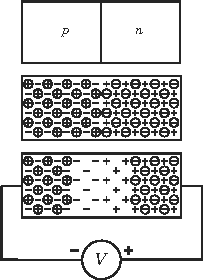
\includegraphics[width=.4\linewidth]{Images/LGADs/p-n junction with voltage.png}
%     \caption{Top: adjacent regions of $p$-doping (left) and $n$-doping forming a $pn$-junction. Middle: the circled mobile charges (holes for $p$-type and electrons for $n$-type) balanced by the charge of atomic cores. Bottom: When an external (reverse) voltage is applied to the central region an electric field builds up in the junction.}
% \end{SCfigure}

%%% WRAPPED FIGURE
% \begin{wrapfigure}{l}{.45\linewidth}
%     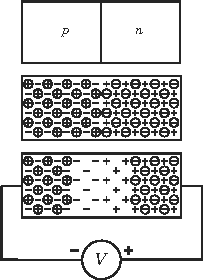
\includegraphics[width=1\linewidth]{Images/LGADs/p-n junction with voltage.png}
%     \caption{Top: adjacent regions of $p$-doping (left) and $n$-doping forming a $pn$-junction. Middle: the circled mobile charges (holes for $p$-type and electrons for $n$-type) balanced by the charge of atomic cores. Bottom: When an external (reverse) voltage is applied to the central region an electric field builds up in the junction.}
%     \label{fig:p-n_junction_reverse_bias_voltage}
% \end{wrapfigure}

%%% FIGURE WITH MINIPAGE
\begin{figure}[!h]
    \begin{minipage}[c]{.25\linewidth}
        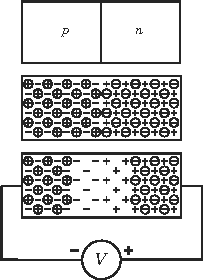
\includegraphics[width=1\linewidth]{Images/LGADs/p-n junction with voltage.png}
    \end{minipage}
    \hfill
    \begin{minipage}[c]{.6\linewidth}
        \caption{\\Top: adjacent regions of $p$-doping (left) and $n$-doping (right) forming a $pn$-junction.\\
        Middle: the circled mobile charges (holes for $p$-type and electrons for $n$-type) balanced by the charge of atomic cores.\\
        Bottom: When an external (reverse) voltage is applied to the junction an electric field builds up in the central region \cite{10.1093/acprof:oso/9780198527848.003.0001}.}
    \end{minipage}
    \label{fig:p-n_junction_reverse_bias_voltage}
\end{figure} 

When a charged particle traverses this depletion layer it frees up electron-hole pairs, which move to the electrodes and can be measured. 

\section{Low Gain Avalanche Detectors}

A particular type of silicon sensors are Low Gain Avalanche Detectors (LGAD), an example is shown is shown in Figure \ref{fig:LGADs_schema}. The major innovation is an additional $p$-type layer below the $n+$ electrode, this creates a high electric field region which leads to an avalanche effect\footnote[2]{When electrons acquire enough energy they can create new electron-hole pairs ('impact ionization'), which can themselves create new pairs and initialize a multiplication chain that leads to an enhanced signal} of the electrons. This effect produces a gain of around $~10$ \marginpar{\flushleft source} 

\begin{figure}[!ht]
    \centering
    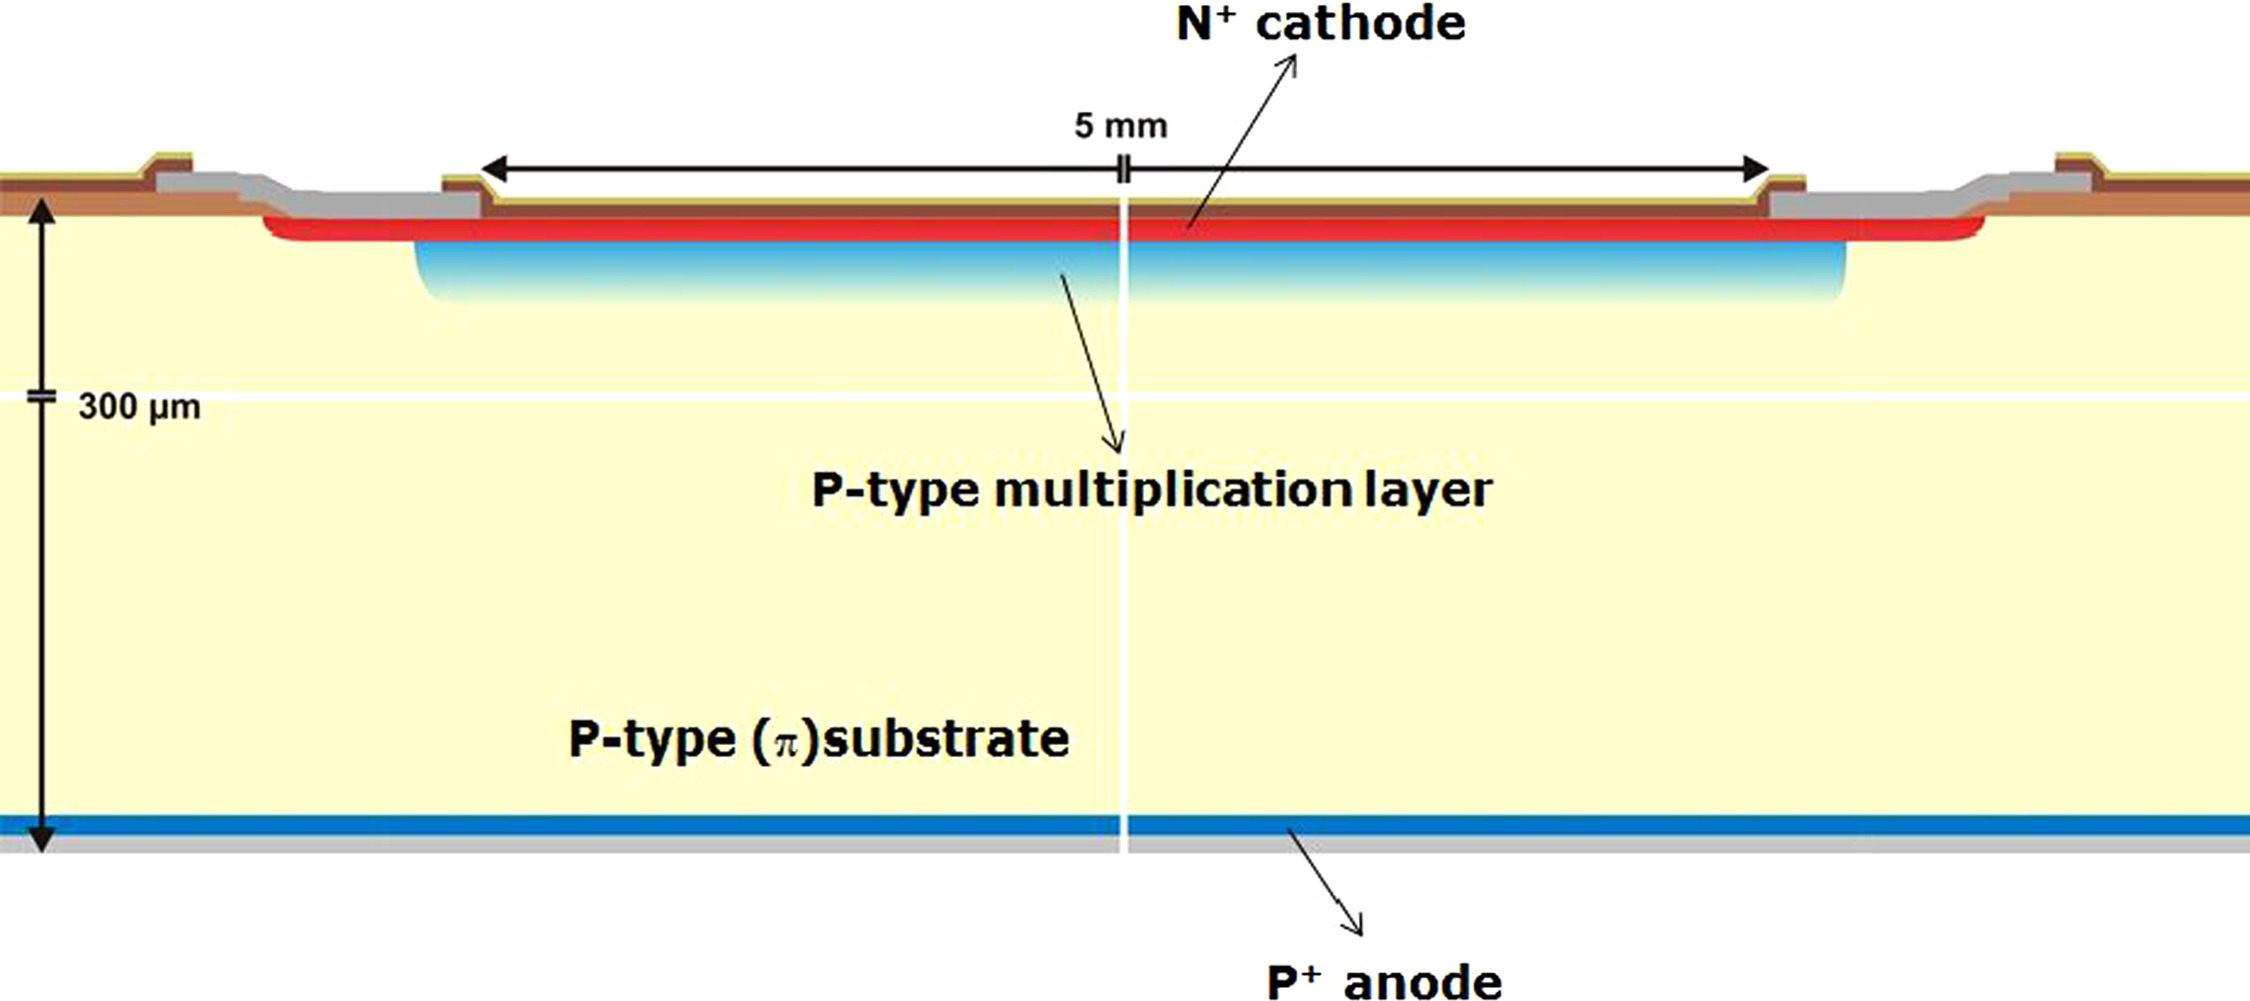
\includegraphics[width=.9\linewidth]{Images/LGADs/1-s2.0-S0168900214007128-gr1_lrg.jpg}
    \caption{description of LGAD}
    \label{fig:LGADs_schema}
\end{figure}

\section{The sensors}
There were several samples that were tested, divided into three main categories of design:
\begin{itemize}
    \item USTC, from the University of Science and Technology of China
    \item IHEP, from the Institute of High Energy Physics, China
    \item CNM, from the Centro National de Microelectronica, Barcelona, Spain
\end{itemize}

the first two designs have both been manufactured by the IME (Institute of Microelectronics) of the Chinese Academy of Sciences. The two CNM sensors (labeled CNM-W4 and CNM-W5) were used to measure the time resolution of another device, the MCP (Section \ref{sec:MCP_description}), which was used as a time reference for all of the time measurements of the other LGADs. Table \ref{tab:devices_tested} provides the list of the devices that were characterized, for more detailed descriptions see Table in \nameref{chap:appendix}.

\begin{table}[!ht]
    \centering
    \caption{Summary of the tested devices}
    \label{tab:devices_tested}
    \scriptsize
    % \makebox[1\textwidth][c]{
    \begin{tabularx}{1\textwidth}{|l|l|l|l|l|X|}
    \hline %%% I NEED TO TRY TO USE TABULAR INSTEAD OF SHORTSTACK
        \textbf{Sevice name} & \textbf{Vendor} & \begin{tabular}{@{}l@{}}\textbf{Pads,} \\ \textbf{used channels}\end{tabular} & \begin{tabular}{@{}l@{}}\textbf{Fluence} \\ $[n_{eq}/\si{cm^2}]$ \end{tabular} & \begin{tabular}{@{}l@{}} \textbf{Radiation} \\ \textbf{type} \end{tabular} & \textbf{Notes} \\
        \hline
        CNM-W4  & CNM & single & 0 & - & reference \\ 
        CNM-W5  & CNM & single & 0 & - & reference \\ 
        CNM-W5-1.5E15  & CNM & single & $\num{1.50E+15}$ & neutron &  \\ 
        CNM-W3-2.5E15  & CNM & single & $\num{2.50E+15}$ & neutron &  \\ 
        USTC2.1-W17 & USTC & 2x2, 2 channels  & 0 & - &  \\ 
        USTC2.1-W17-2E14 & USTC & 2x2, 1 channel & 0 & - & missing \\ 
        IMEv3-W12-2x2  & IHEP & 2x2, 2 channels  & 0 & - &  \\ 
        IMEv3-W12-1x3  & IHEP & 1x3, 2 channels  & 0 & - &  \\ 
        IMEv3-W12  & IHEP & 2x2, 3 channels  & $\num{1.50E+15}$ & neutron &  \\ 
        IMEv3-W16  & IHEP & 1x3, 1 channel  & $\num{1.50E+15}$ & neutron &  \\ 
        IMEv2-W7-1E14  & IHEP & single & $\num{1.00E+14}$ & proton &  \\ 
        IMEv2-W7-6.5E14  & IHEP & single & $\num{6.50E+14}$ & proton &  \\ 
        IMEv3-W16-8E14  & IHEP & single & $\num{8.00E+14}$ & proton &  \\
        IMEv3-W16-2.5E15  & IHEP & single & $\num{2.50E+15}$ & neutron &  \\ 
        \hline
    \end{tabularx}
\end{table}




%%% NOT UPDATED ANYMORE, LOOK AT THE EXCEL FILE, I MIGHT DELETE THIS LATER
%%% I have to reorganize these and associate them with the more accurate descriptions
% device name:        vendor:        sensor ID:            fluence:    irradiation type:    type:        board name:    channels:
% CNM-W4              CNM          CNM-R15973-W4-D168      unirradiated      -             single pad     JSI-B12      1
% CNM-W5              CNM          CNM-R15973-W5-D138      unirradiated      -             single pad     JSI-B14      1
% CNM-W3-2.5E15       CNM          CNM-R15973-W3-D29       $\num{2.5e15}     neutron       single pad     JSI B5       1
% CNM-W5-1.5E15       CNM          CNM-R15973-W5-D29       $\num{1.5e15}     neutron       single pad     JSI PP1      1
% USTC2.1             USTC         USTC2.1-W17-P6-A          0                -             2x2           CERN-3       1,2
% USTC2.1 IRRADIATED (MISSING)
% IMEv3-W12-C2         IHEP        IMEv3-W12-C2-2-2          0               -              2x2          CERN-1       channels 1,2
% IMEv3-W12-C3         IHEP        IMEv3-W12-C3-1-4 (and 5)  0               -              1x3          CERN-1       channles 3,4  (small GR), bonded
% CERN2-CH0-IMEv3-W12  IHEP        IMEv3-W12-B2-2-9-1       1.5e15           neutron        2x2 sensor    CERN-2       channels 1,2,3
% CERN2-CH1-IMEv3-W12  IHEP 
% CERN2-CH2-IMEv3-W12  IHEP 
% CERN2-CH4-IMEv3-W16  IHEP        IMEv3-W16-Q4-D4-1-4      1.5e15           neutron        1x3          CERN-2       channel:  2(?)
% JSI-B6-IMEv2-W7-1E14    IHEP       W7-II-C2-1-7 IMEv2-W7Q2    1e14          proton        single       JSI-B6
% JSI-PP4-IMEv2-W7-6.5E14 IHEP       W7-II-C2-1-7 IMEv2-W7Q2    6.5e14        proton        single       JSI-PP4
% JSI-B7-IMEv3-W16-8E14   IHEP       IHEP-IMEv3-W16_Q4_D3_1-4   8e14          (unsure)        single       JSI-B7
% JSI-B13-IMEv3-W16-2.5E15 IHEP      IHEP-IMEv3-W16_Q4_E3_1-4   2.5e15       (unsure)      single        JSI-B13
                 

\chapter{Test Beam setup}\label{chap:testbeam_setup}

%%% motivate testbeam
A typical way to test the performance of sensors for High-Energy Physics applications is with test beams: the Devices Under Test (DUTs) are put through a focused flux of high energy particles and their response is read out and analyzed. %%% aka testbeam

The HGTD collaboration has run many test beam campaigns, mainly at CERN and at DESY (Deutsches Elektronen-Synchrotron). The focus of this analysis is the test beam campaign of May 2023, conducted at CERN using a beam of \qty{120}{\giga\electronvolt} pions, provided by SPS.

\begin{figure}[h!tbp]
    \centering
    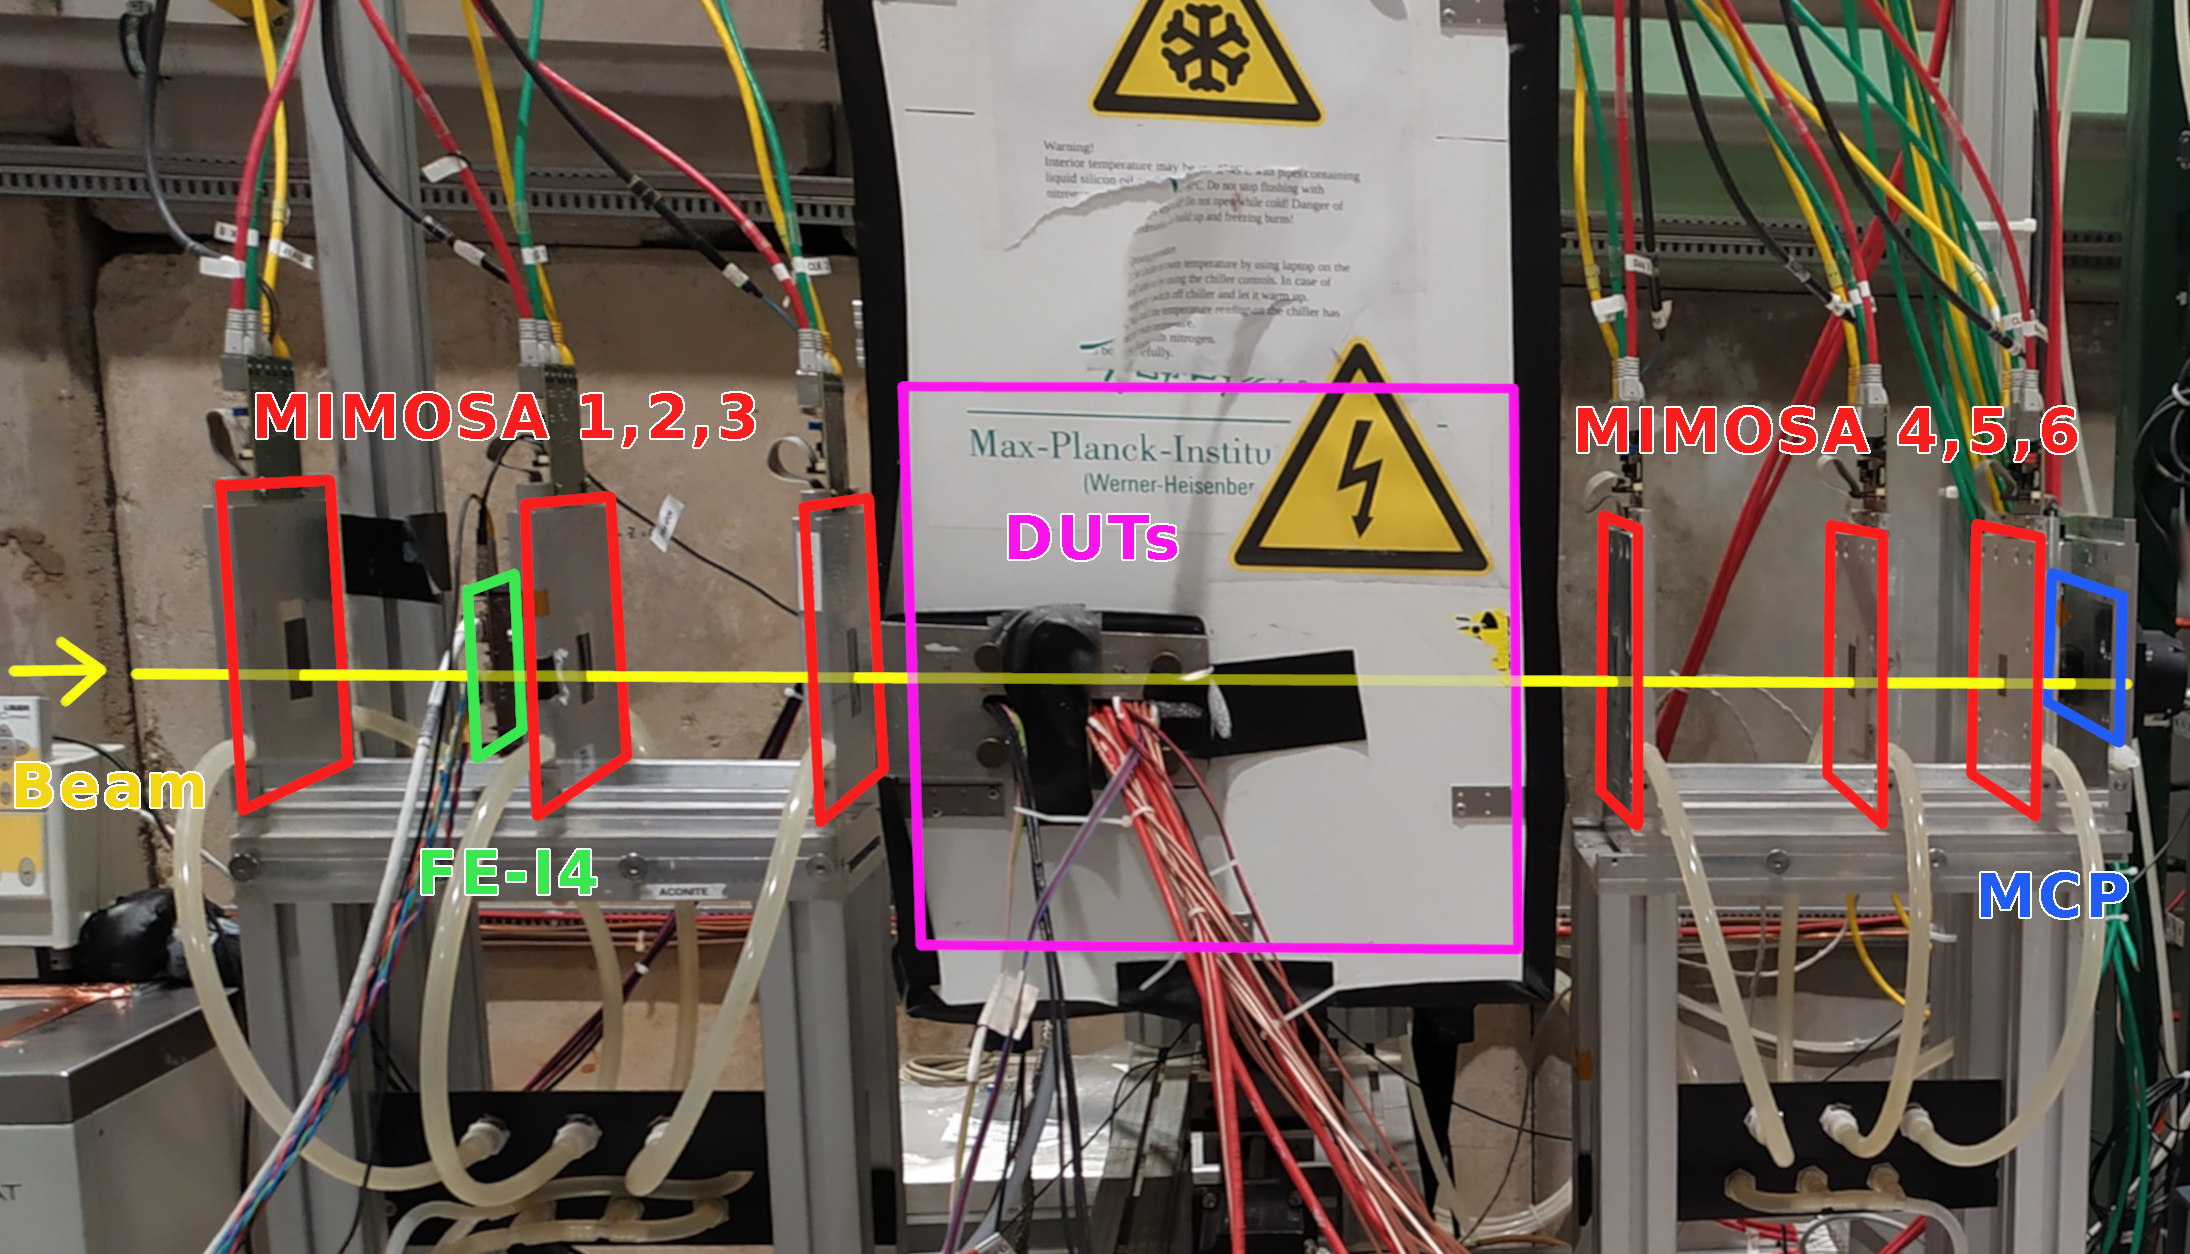
\includegraphics[width=.95\linewidth]{Images/TestBeam_setup/TestBeam_setup_redrawn.png}
    \captionsetup{width=\captionwidth}
    \caption{The main components of the test beam setup: the EUDET-type beam telescope with six MIMOSA planes, the FE-I4, the MCP and the cooling box containing the DUTs}
    \label{fig:testbeam_setup}
\end{figure}

The experimental setup of this campaign included:
\begin{itemize}
    \item FE-i4~\cite{Obermann:2014goa}: a hybrid pixel detector that provided a user-defined Region Of Interest (ROI), creating a HitOR\footnote{A binary signal generated when at least one pixel registers a hit} signal. %to avoid noisy pixels.
    \item Trigger Logic Unit (TLU): provided a trigger\footnote{A trigger is a signal that initiates data readout when a particle is detected}, combining the signals from a scintillator and the FE-i4. %% describe trigger??
    \item EUDET-type beam telescope equipped with 6 MIMOSA planes~\cite{Jansen:2016bkd}: used for precise spatial measurements of the particles in the beam, enabling track reconstruction.
    \item MicroChannel Plate detector (MCP)~\cite{LADISLASWIZA1979587}: measured the time of the moving particles, used as reference for the time resolution.
    \item Cooling box: contained the various DUTs, maintaining them at \qty{-30}{\degreeCelsius}.
    \item 2 oscilloscopes: acquired the data from the MCP and the DUTs. %%% I put later the channels
\end{itemize}

%%% maybe this should just be later

% description of components:
% • Trigger logic unit for particle passing
% • FEi4 to select a region of interest
% • Mimosa planes for tracking (X and Y position data)
% • MCP for time reference 
% • Cooling box containint the DUTs, (can be tilted with respect to the beam direction)
% • 120 GeV beam of pion

\section{TLU and FEi4}

The Trigger Logic Unit provided a trigger whenever a particle was detected. This trigger in turn instructed various components (in this case the oscilloscopes, the MIMOSA planes) to initiate data acquisition. More specifically the TLU took input from a scintillator and the FE-i4 to create a trigger.

The FE-i4 (Front-End-Iteration 4)~\cite{Obermann:2014goa} is a pixel readout chip with a planar silicon sensor bump bonded to it. It has a configurable sensitive area of up to \(\num{16.8} \times \qty{20}{\milli\meter^2}\) made up of 80 columns (\qty{250}{\micro\meter} pitch) and 336 rows (\qty{50}{\micro\meter}). 

Selecting a specific ROI allowed to exclude the areas outside the DUTs surface and to reduce sources of noise (e.g. noisy pixels of MIMOSA planes). %%% maybe the next part is just a repetition of what I say later
%It should be noted that in some occasions, due to erroneous ROI selection or due to small positional shifts caused by temperature fluctuations, the DUTs fell outside said ROI and the analysis was negatively impacted. (Example in Appendix, later)

\section{EUDET-type beam telescope}
A EUDET-type beam telescope~\cite{Jansen:2016bkd} equipped with a total of 6 Minimum Ionizing MOS Active Pixel Sensor planes~\cite{Hu-Guo:2010lrq} provided precise spatial measurements of particle trajectories. Each plane consists of 576 rows and 1152 columns of pixels, each sized \(\qty{18.4}{\micro\meter} \times \qty{18.4}{\micro\meter}\), covering an active area of around \(\num{21.2} \times \qty{10.6}{\micro\meter^2}\). Three of the planes were located before the DUTs, in the direction of the beam, and three were located after. The hits provided by the planes enabled the reconstruction of the tracks of the particles in the beam.

\section{MCP}\label{sec:MCP_description}
The microchannel plate (MCP) detector~\cite{LADISLASWIZA1979587} consists of a single block of resistive material with numerous evenly spaced small tubes (microchannels) connecting one face to the other. The main working principle is similar to that of an electron multiplier. When a voltage is applied between the two sides a potential gradient is established along the channels. Whenever a charged particle hits the inner wall of the tubes multiple secondary electrons are emitted, these electrons then are accelerated and hit the opposite wall in the channel, causing the emission of further secondary electrons. As a result, an exponentially increasing number of electrons can be extracted from the output. This detector can provide very fast response time and, for this reason, it was used as a reference for the time resolution of the other devices.


\begin{figure}
\begin{minipage}[c]{.45\linewidth}
    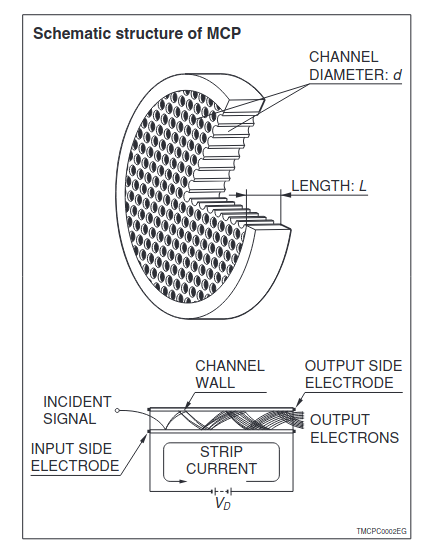
\includegraphics[width=1\linewidth]{Images/TestBeam_setup/MCP diagram HAMAMATSU.png}
\end{minipage}
\hfill
\begin{minipage}[c]{.5\linewidth}
    \caption{
    Schematics of an MCP.\\ 
    Top: structure of the detector with a cross-sectional view of the channels, highlighting the diameter \(d\) and the length \(L\) of the micro-channels. Standard MCPs are fabricated with a diameter of \(10\)s \unit{\micro\meter} and a ratio \(\alpha\) (\(\alpha = L / d\)) 40 to 60.\\
    Bottom: when a voltage (\(V_D\)) is applied, the channel walls behave as continuous electron multiplier: when a target object (electron, ion or photon) hits the inner walls, electrons are released in a parabolic trajectory, and they start a chain reaction which produces a signal amplified by \(10^4-10^7\) times. From~\cite{MCP_figure}.}
\end{minipage}
\label{fig:MCP_diagrame}
\end{figure}


\subsection{Time resolution of the MCP}
The time resolution of the MCP was first calculated by comparing the time difference of two independent sensors (CNM-W4 and CNM-W5, described in Section~\ref{sec:the_sensors}) and the MCP. In this way, it was possible to build a system of three equations of the time differences.

\begin{equation}\label{eq:time_res_system_eqs}
    \begin{cases}
        t_{1-2} = t_1 - t_2  \\
        t_{1-MCP} = t_1 - t_{MCP} \\
        t_{2-MCP} = t_2 - t_{MCP} \, .
    \end{cases}
\end{equation}

The time distributions (left sides of the equations) were fitted with a Gaussian function, each with a width \(\sigma_{ij} = \sigma_i \oplus \sigma_j\), where \(i\) and \(j\) are two of the devices in Equation~\ref{eq:time_res_system_eqs} (i.e. MCP, CNM-W4 and CNM-W5). Assuming that the devices were all independent, their time resolutions would also be independent. This gave a system of three equations with three unknowns, which could be solved analytically to find each individual time resolution: \(\sigma_1\), \(\sigma_2\), \(\sigma_{MCP}\).

This procedure was repeated for all available runs, and the results computed this way are shown in Table \ref{tab:MCP_time_resolution}.
\begin{table}[h!tbp]
    \begin{center}
        \captionsetup{width=\captionwidth}
        \caption{Time resolution values of the MCP. The uncertainty is the standard deviation of all the computed runs.}
        \label{tab:MCP_time_resolution}
        \begin{tabular}{ | c | c | c | c | }
            \hline
            Voltage [\(\si{V}\)] & 2500 & 2600 & 2800 \\ 
            \hline 
            Time resolution [\(\si{ps}\)] & 36.52 & 16.48 & 3.73 \\  
            Uncertainty [\(\si{ps}\)] & \(\pm\)0.81 & \(\pm\)0.57 & \(\pm\)1.33 \\
            \hline
        \end{tabular}
    \end{center}
\end{table}


\section{Oscilloscopes}
The signal generated by the DUT was recorded by two four-channel oscilloscopes: channel 1 (denoted as Ch1) of both oscilloscopes was connected to the MCP (whose signal was put through a splitter and sent to both oscilloscopes). Therefore, up to 6 channels were available in each batch to be attached to the DUTs.
The waveforms recorded by the oscilloscopes were then processed with the PyAna software~\cite{atlas_hgtd_pyana_2025}. 
%  \marginpar{\flushleft I explain this later in the methods}


\section{The sensors}\label{sec:the_sensors}
A variety of LGADs were tested: with different manufacturers, different designs and different fluence\footnote{Radiant exposure, here measured in neutron-equivalent over square centimeters}. They were divided into three main categories:
\begin{itemize}
    \item USTC: from the University of Science and Technology of China.
    \item IHEP: from the Institute of High Energy Physics, China.
    \item CNM: from the Centro Nacional de Microelectr\'onica, Barcelona, Spain.
\end{itemize}

The first two designs have both been manufactured by the IME (Institute of Microelectronics) of the Chinese Academy of Sciences. The two unirradiated CNM sensors (labeled CNM-W4 and CNM-W5) were used to measure the time resolution of another device, the MCP (Section~\ref{sec:MCP_description}), which was used as a time reference for the time measurements of all the other LGADs. 

Two other devices from CNM were irradiated at \qty{1.5e15}{\neutroneq} and \qty{2.5e15}{\neutroneq}. Two versions (v2 and v3) of the IME-IHEP sensors were available, both had a carbon implantation, which has the purpose of increasing the radiation hardness of the LGAD. The sensors were either a single pad or an array (2\(\times\)2 or 1\(\times\)3) of pads, and they were irradiated at fluences ranging from \(0\) to \qty{2.5e15}{\neutroneq}. Two USTC devices, also with carbon enrichment (version 2.1), were tested at zero and low fluence. 

Notably, the data from the irradiated USTC sensor was not available. Moreover, one pad of IMEv3-W12-2x2-1.5E15 was removed from the analysis due a possible wrong labeling (see in Appendix~\ref{sec:mislabeled_sensor}).

The sensors were then installed onto readout boards. In the case of multi-pads sensors, some number of pads were each connected to one channel of the board, so that they could be measured individually.

Table \ref{tab:devices_tested} provides the list of the devices that were characterized.

%%% for more detailed descriptions see Table in \nameref{chap:appendix}.
%%% TODO: maybe more complete table in appendix? with devices id

\begin{table}[h!tbp]  
    \centering
    \captionsetup{width=\captionwidth}
    \caption{List of the tested devices.}
    \label{tab:devices_tested}

    % \makebox[1\textwidth][c]{
    \begin{tabular}{|l|l|l|l|l|l|}
    \hline %%% I NEED TO TRY TO USE TABULAR INSTEAD OF SHORTSTACK
        \textbf{Device name} & \textbf{Vendor} & \begin{tabular}{@{}l@{}}\textbf{Pads,} \\ \textbf{used channels}\end{tabular} & \begin{tabular}{@{}l@{}}\textbf{Fluence} \\ \([n_{eq}/\si{cm^2}]\) \end{tabular} & \begin{tabular}{@{}l@{}} \textbf{Radiation} \\ \textbf{type} \footnotemark \end{tabular}& \textbf{Notes} \\
        \hline
        CNM-W4  & CNM & single & 0 & - & reference \\ 
        CNM-W5  & CNM & single & 0 & - & reference \\ 
        CNM-W5-1.5E15  & CNM & single & \(\num{1.50E+15}\) & neutron & - \\ 
        CNM-W3-2.5E15  & CNM & single & \(\num{2.50E+15}\) & neutron & - \\ 
        USTC2.1-W17 & USTC & 2\(\times\)2, 2 channels  & 0 & - & - \\ 
        USTC2.1-W17-2E14 & USTC & 2\(\times\)2, 1 channel & 0 & - & not available\\ 
        IMEv3-W12-2x2  & IHEP & 2\(\times\)2, 2 channels  & 0 & - & \\ 
        IMEv3-W12-1x3  & IHEP & 1\(\times\)3, 2 channels  & 0 & -  &\\ 
        IMEv3-W12-2x2-1.5E15 & IHEP & 2\(\times\)2, 3 channels  & \(\num{1.50E+15}\) & neutron & only two channels \\ 
        IMEv2-W7-1E14  & IHEP & single & \(\num{1.00E+14}\) & proton & -\\ 
        IMEv2-W7-6.5E14  & IHEP & single & \(\num{6.50E+14}\) & proton  & - \\ 
        IMEv3-W16-8E14  & IHEP & single & \(\num{8.00E+14}\) & proton & - \\
        IMEv3-W16-1x3-1.5E15  & IHEP & 1\(\times\)3, 1 channel  & \(\num{1.50E+15}\) & neutron & no usable batches \\ 
        IMEv3-W16-2.5E15  & IHEP & single & \(\num{2.50E+15}\) & neutron  & - \\ 
        \hline
    \end{tabular}
\end{table}

\footnotetext{\label{footnote:radiation_type} As protons and neutrons interact differently with the atoms of the silicon lattice, they can introduce distinct defect structures. In addition, the enrichment of various impurities may lead to further differences in the type of damage \cite{Ruzin:1999ck}.}

%%% NOT UPDATED ANYMORE, LOOK AT THE EXCEL FILE, I MIGHT DELETE THIS LATER
%%% I have to reorganize these and associate them with the more accurate descriptions
% device name:        vendor:        sensor ID:            fluence:    irradiation type:    type:        board name:    channels:
% CNM-W4              CNM          CNM-R15973-W4-D168      unirradiated      -             single pad     JSI-B12      1
% CNM-W5              CNM          CNM-R15973-W5-D138      unirradiated      -             single pad     JSI-B14      1
% CNM-W3-2.5E15       CNM          CNM-R15973-W3-D29       $\num{2.5e15}     neutron       single pad     JSI B5       1
% CNM-W5-1.5E15       CNM          CNM-R15973-W5-D29       $\num{1.5e15}     neutron       single pad     JSI PP1      1
% USTC2.1             USTC         USTC2.1-W17-P6-A          0                -             2\(\times\)2           CERN-3       1,2
% USTC2.1 IRRADIATED (MISSING)
% IMEv3-W12-C2         IHEP        IMEv3-W12-C2-2-2          0               -              2\(\times\)2          CERN-1       channels 1,2
% IMEv3-W12-C3         IHEP        IMEv3-W12-C3-1-4 (and 5)  0               -              1x3          CERN-1       channles 3,4  (small GR), bonded
% CERN2-CH0-IMEv3-W12  IHEP        IMEv3-W12-B2-2-9-1       1.5e15           neutron        2\(\times\)2 sensor    CERN-2       channels 1,2,3
% CERN2-CH1-IMEv3-W12  IHEP 
% CERN2-CH2-IMEv3-W12  IHEP 
% CERN2-CH4-IMEv3-W16  IHEP        IMEv3-W16-Q4-D4-1-4      1.5e15           neutron        1x3          CERN-2       channel:  2(?)
% JSI-B6-IMEv2-W7-1E14    IHEP       W7-II-C2-1-7 IMEv2-W7Q2    1e14          proton        single       JSI-B6
% JSI-PP4-IMEv2-W7-6.5E14 IHEP       W7-II-C2-1-7 IMEv2-W7Q2    6.5e14        proton        single       JSI-PP4
% JSI-B7-IMEv3-W16-8E14   IHEP       IHEP-IMEv3-W16_Q4_D3_1-4   8e14          (unsure)        single       JSI-B7
% JSI-B13-IMEv3-W16-2.5E15 IHEP      IHEP-IMEv3-W16_Q4_E3_1-4   2.5e15       (unsure)      single        JSI-B13
                 

\chapter{Analysis}\label{chap:methods}
%%% I need to restructure deeply

The data recorded by the oscilloscopes, in the form of waveforms, was pre-processed using the software PyAna~\cite{atlas_hgtd_pyana_2025}. Another software, PaTrack~\cite{atlas_hgtd_patrack_2025}, used the spacial information from the MIMOSA planes to reconstruct the tracks of the particles. The data was then combined into ROOT files to be further analyed.


Some quality cuts were applied to the data, to remove extra noise. To illustrate the analysis procedure that was followed in this study, a single DUT was picked as an example. All the plots in this chapter (unless otherwise stated) refer to the sensor IMEv3-W12, a 2\(\times\)2 array of LGADs, operated at \qty{-30}{\degreeCelsius} and perpendicular to the beam.

\section{Data pre-processing}

The pre-processing was performed by other collaborators prior to this analysis. The steps of the pre-processing are described below.

\begin{figure}[h!btp]
    \centering
    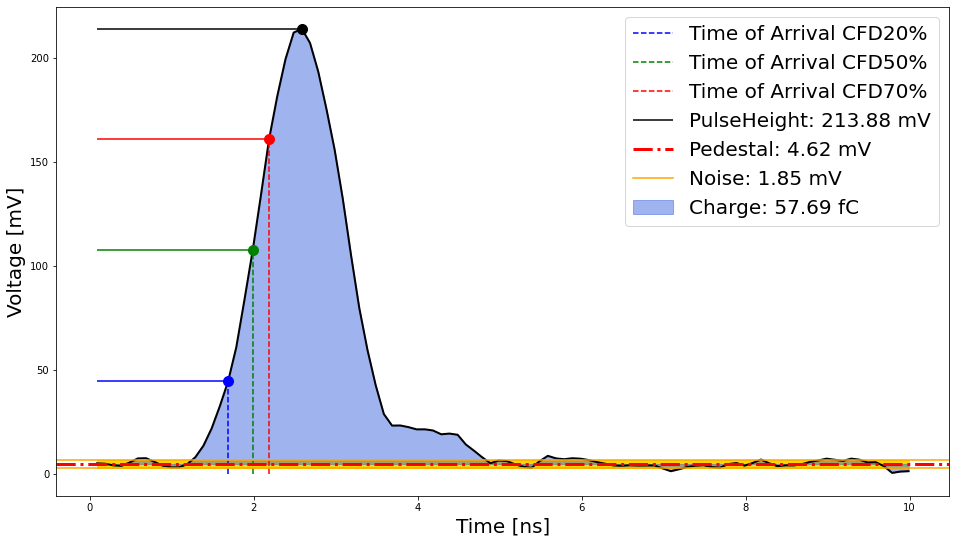
\includegraphics[width=1\linewidth]{Images/methods/Waveform of particle, channel2, with CFD (ns).png}
    \captionsetup{width=\captionwidth}
    \caption{An example of a pulse with its main features highlighted. The pedestal (red dotted line) is the mean of the background signals, the noise (yellow) is its standard deviation, the pulseheight (black) is the maximum amplitude and the charge (light blue) is the area under the pulse. The remaining three dashed lines (blue, green and red) correspond to the TOA associated to three different values of CFD (20\%, 50\% and 70\%, respectively).}
    \label{fig:waveform_features}
\end{figure} 

%PyAna, aka pulse description
Whenever a trigger was detected, the oscilloscopes recorded an event. For each event, at least 2000 samples were collected, spaced every \qty{25}{\pico\second}, an example of one event (a pulse) is shown in Figure~\ref{fig:waveform_features}. This pulse (waveform) was then processed with PyAna.

Firstly, the pedestal and the noise were measured by computing the mean and standard deviation, respectively, using the first 240 samples, where no signal is expected \cite{Allaire:2018bof}. Secondly, the maximum of the pulse was found by a second-degree polynomial fit, in a \qty{400}{\pico\second} window around the sample with the highest amplitude. After subtracting the pedestal, the total charge was computed as the integral of the pulse divided by the transimpedance\footnote{Trasfer impedance, it is the ratio of output voltage to input current in the readout board, expressed in \unit{\ohm}} value of the board the LGAD is mounted on (Equation~\ref{eq:charge_integral}). The integral is computed in a window wide enough to contain the full pulse.

\begin{equation}\label{eq:charge_integral}
    Q = \frac{\int_{t_1}^{t_2} V(t)dt}{R_b} \, .
\end{equation}
Where \(Q\) is the charge, \(V\) is the voltage (as a function of time \(t\)), \(R_b\) is the transimpedance and \(t_2-t_1\) is the integration window.

%%% PaTrack, aka MIMOSA plane
The spacial information was processed with the PaTrack software to create tracks of the particles. Two straight tracklets, an "upstream" and a "downstream" tracklet passing through MIMOSA planes 1,2,3 and 4,5,6, respectively, were reconstructed to best fit the hits on each plane and meet at the longitudinal (z) location of the DUTs, Figure~\ref{fig:mimosa_tracking}. This provided each event with the XY intersection of the track onto the plane of each DUT. 

\begin{figure}[h!btp]
    \centering
    \includegraphics[width=1\linewidth]{Images/methods/MIMOSA tracking scheme.png}
    \captionsetup{width=\captionwidth}
    \caption{Scheme of the reconstructed tracks, made of two tracklets, one upstream and one upstream, as they best fit the hits on the MIMOSA planes before and after the DUTs.}
    \label{fig:mimosa_tracking}
\end{figure} 


To measure the time resolution it is crucial to define the Time of Arrival (TOA), i.e. the time at which the particle hits the sensor and the pulse is recorded. There are several ways to make this choice, including: Constant Threshold Discriminator (CTD), Constant Fraction Discriminator (CFD) and Zero Crossing Detector (ZCD).

\begin{figure}[h!btp]
    \centering
    \includegraphics[width=.8\linewidth]{Images/methods/Constant_fraction_1.pdf}
    \captionsetup{width=\captionwidth}
    \caption{Comparison of Constant Threshold Discriminator (left) and Constant Fraction Discriminator (right), for two pulses with similar shapes but different amplitudes. CTD has a fixed threshold value, the TOA \(t\) is set when the pulse crosses the threshold. For CFD, the time \(t\) corresponds to the moment the pulse reaches a certain fraction of the maximum amplitude. This illustrates the \textit{time walk} effect.}
    \label{fig:constant fraction}
\end{figure} 

In this study we chose to use the Constant Fraction Discriminator. More specifically, for the MCP a value of 50\% CFD was chosen, while for the DUTS a value of 20\% was chosen in all cases except for heavily irradiated sensors, in which 70\% yielded improved results overall.

\FloatBarrier

\section{Quality cuts}\label{sec:qualtiy_cuts}

% To remove the various sources of noise some quality cuts were applied to the data. %; in this section we explain these choices.
To ensure that only physically meaningful events were used in the measurements, it was necessary to apply some quality cuts to the initial data. These cuts were designed to reject events affected by various sources of noise or not meaningful to the analysis. 
%%% TODO: maybe more examples? 

To begin with, we removed events with low signal peak (or high noise). Subsequently, we used the pulse height information to identify the outline of each pad and select only events passing through it. Finally, we established a time window around the peak of the distribution to avoid negative effects caused by the neighbouring pads and the edges of the sensors (outside the gain layer).

\subsection{Noise cut}\label{subsec:noise_cut}
The most straightforward trimming consisted in the exclusion of signals which had a pulseheight less than 3 times greater than the noise:

\begin{equation*}
    P > b + 3\sigma \, .
\end{equation*}

Where \(P\) is the maximum of the pulse (pulseheight), \(b\) is pedestal baseline and \(\sigma\) is the noise. This ensured the exclusion of events that could simply be particularly highly peaked noise. %%% don't know about this sentence

\subsection{Pulse height cut}\label{subsec:pulseHeight_cut}

% I think I want to cut out the title
\begin{figure}[h!tbp]
    \centering
    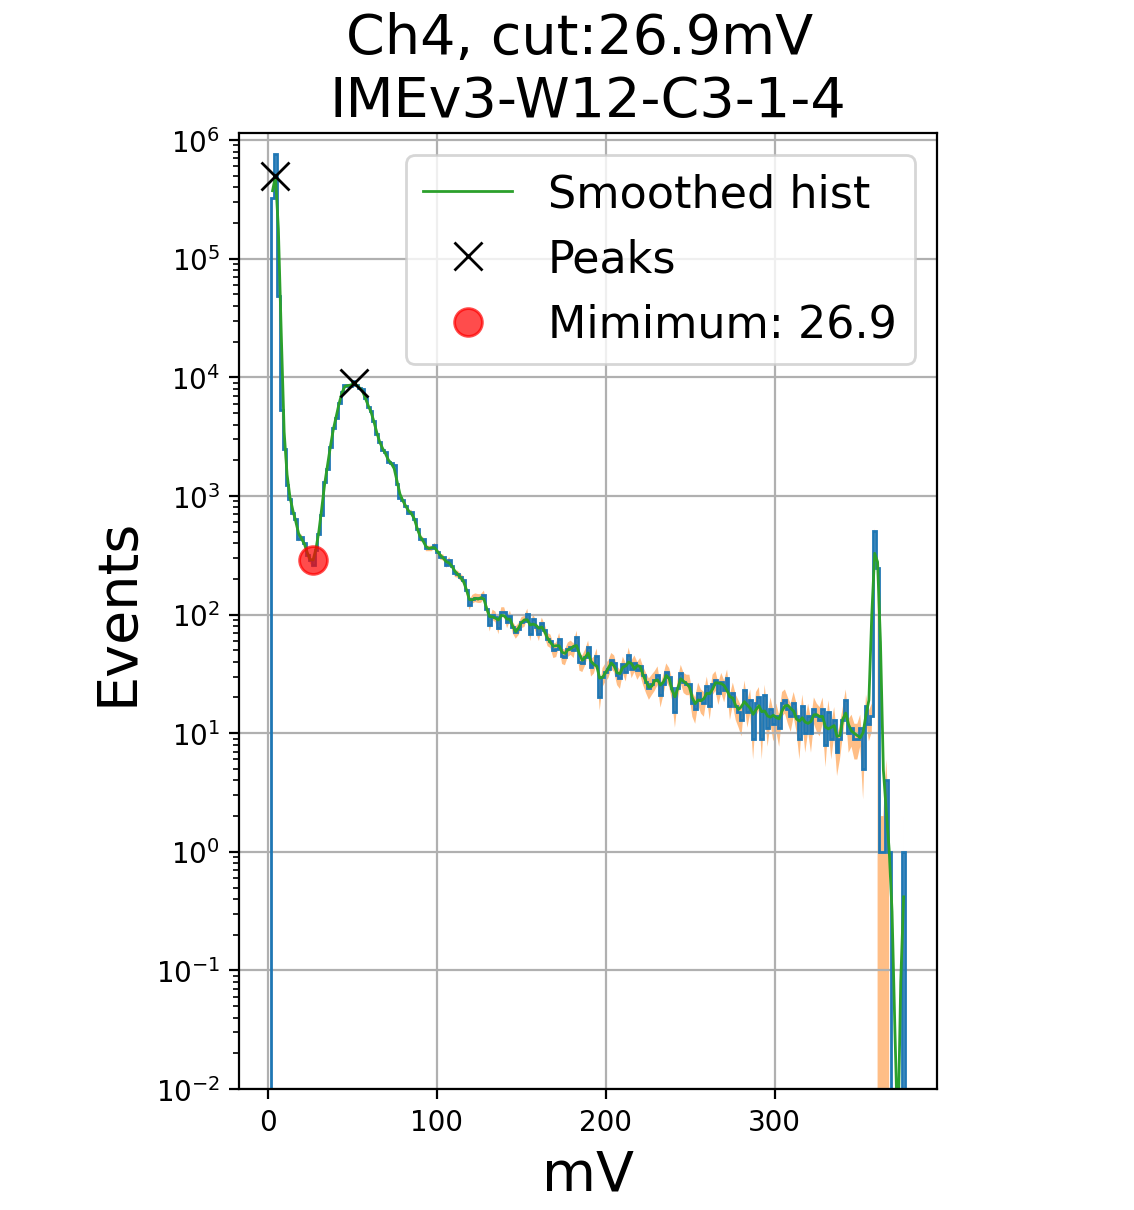
\includegraphics[width=.5\linewidth]{Images/methods/2D_Sensors_401 S1 pulseHeight cut_pulse.png}
    \captionsetup{width=\captionwidth}
    \caption{The pulse height cut was defined by the position of the local minimum between the two main peaks (identified as to noise and signal)}
    \label{fig:pulseHeight_cut}
\end{figure}

By plotting the distribution of pulse height values, we applied a cut to the pulses located below the local minimum in the distribution\footnote{A Kernel Density Estimator was used in order to smooth the distribution before identifying the minimum}, to separate guaranteed signals from potential noise. The goal of this cut was to select only events that were detected by the DUT, and use this information to find the physical outline of the pad.

Using this selection of events, the X and Y coordinates of the tracks were plotted, giving the result shown in Figure~\ref{fig:pulseHeight_cut_highlight}. The outline of the sensor is distinctly shown, making possible the subsequent quality cut: the selection of tracks that passed through the surface of the pad, i.e. a \textit{geometry cut}

\subsection{Geometry cut}\label{sec:geometry_cut}

\begin{figure}[h!tbp]
    \centering
    % \includesvg[width=1\linewidth]{Images/methods/locating_edges_Xtr_batch_401_S1_DUT3}
    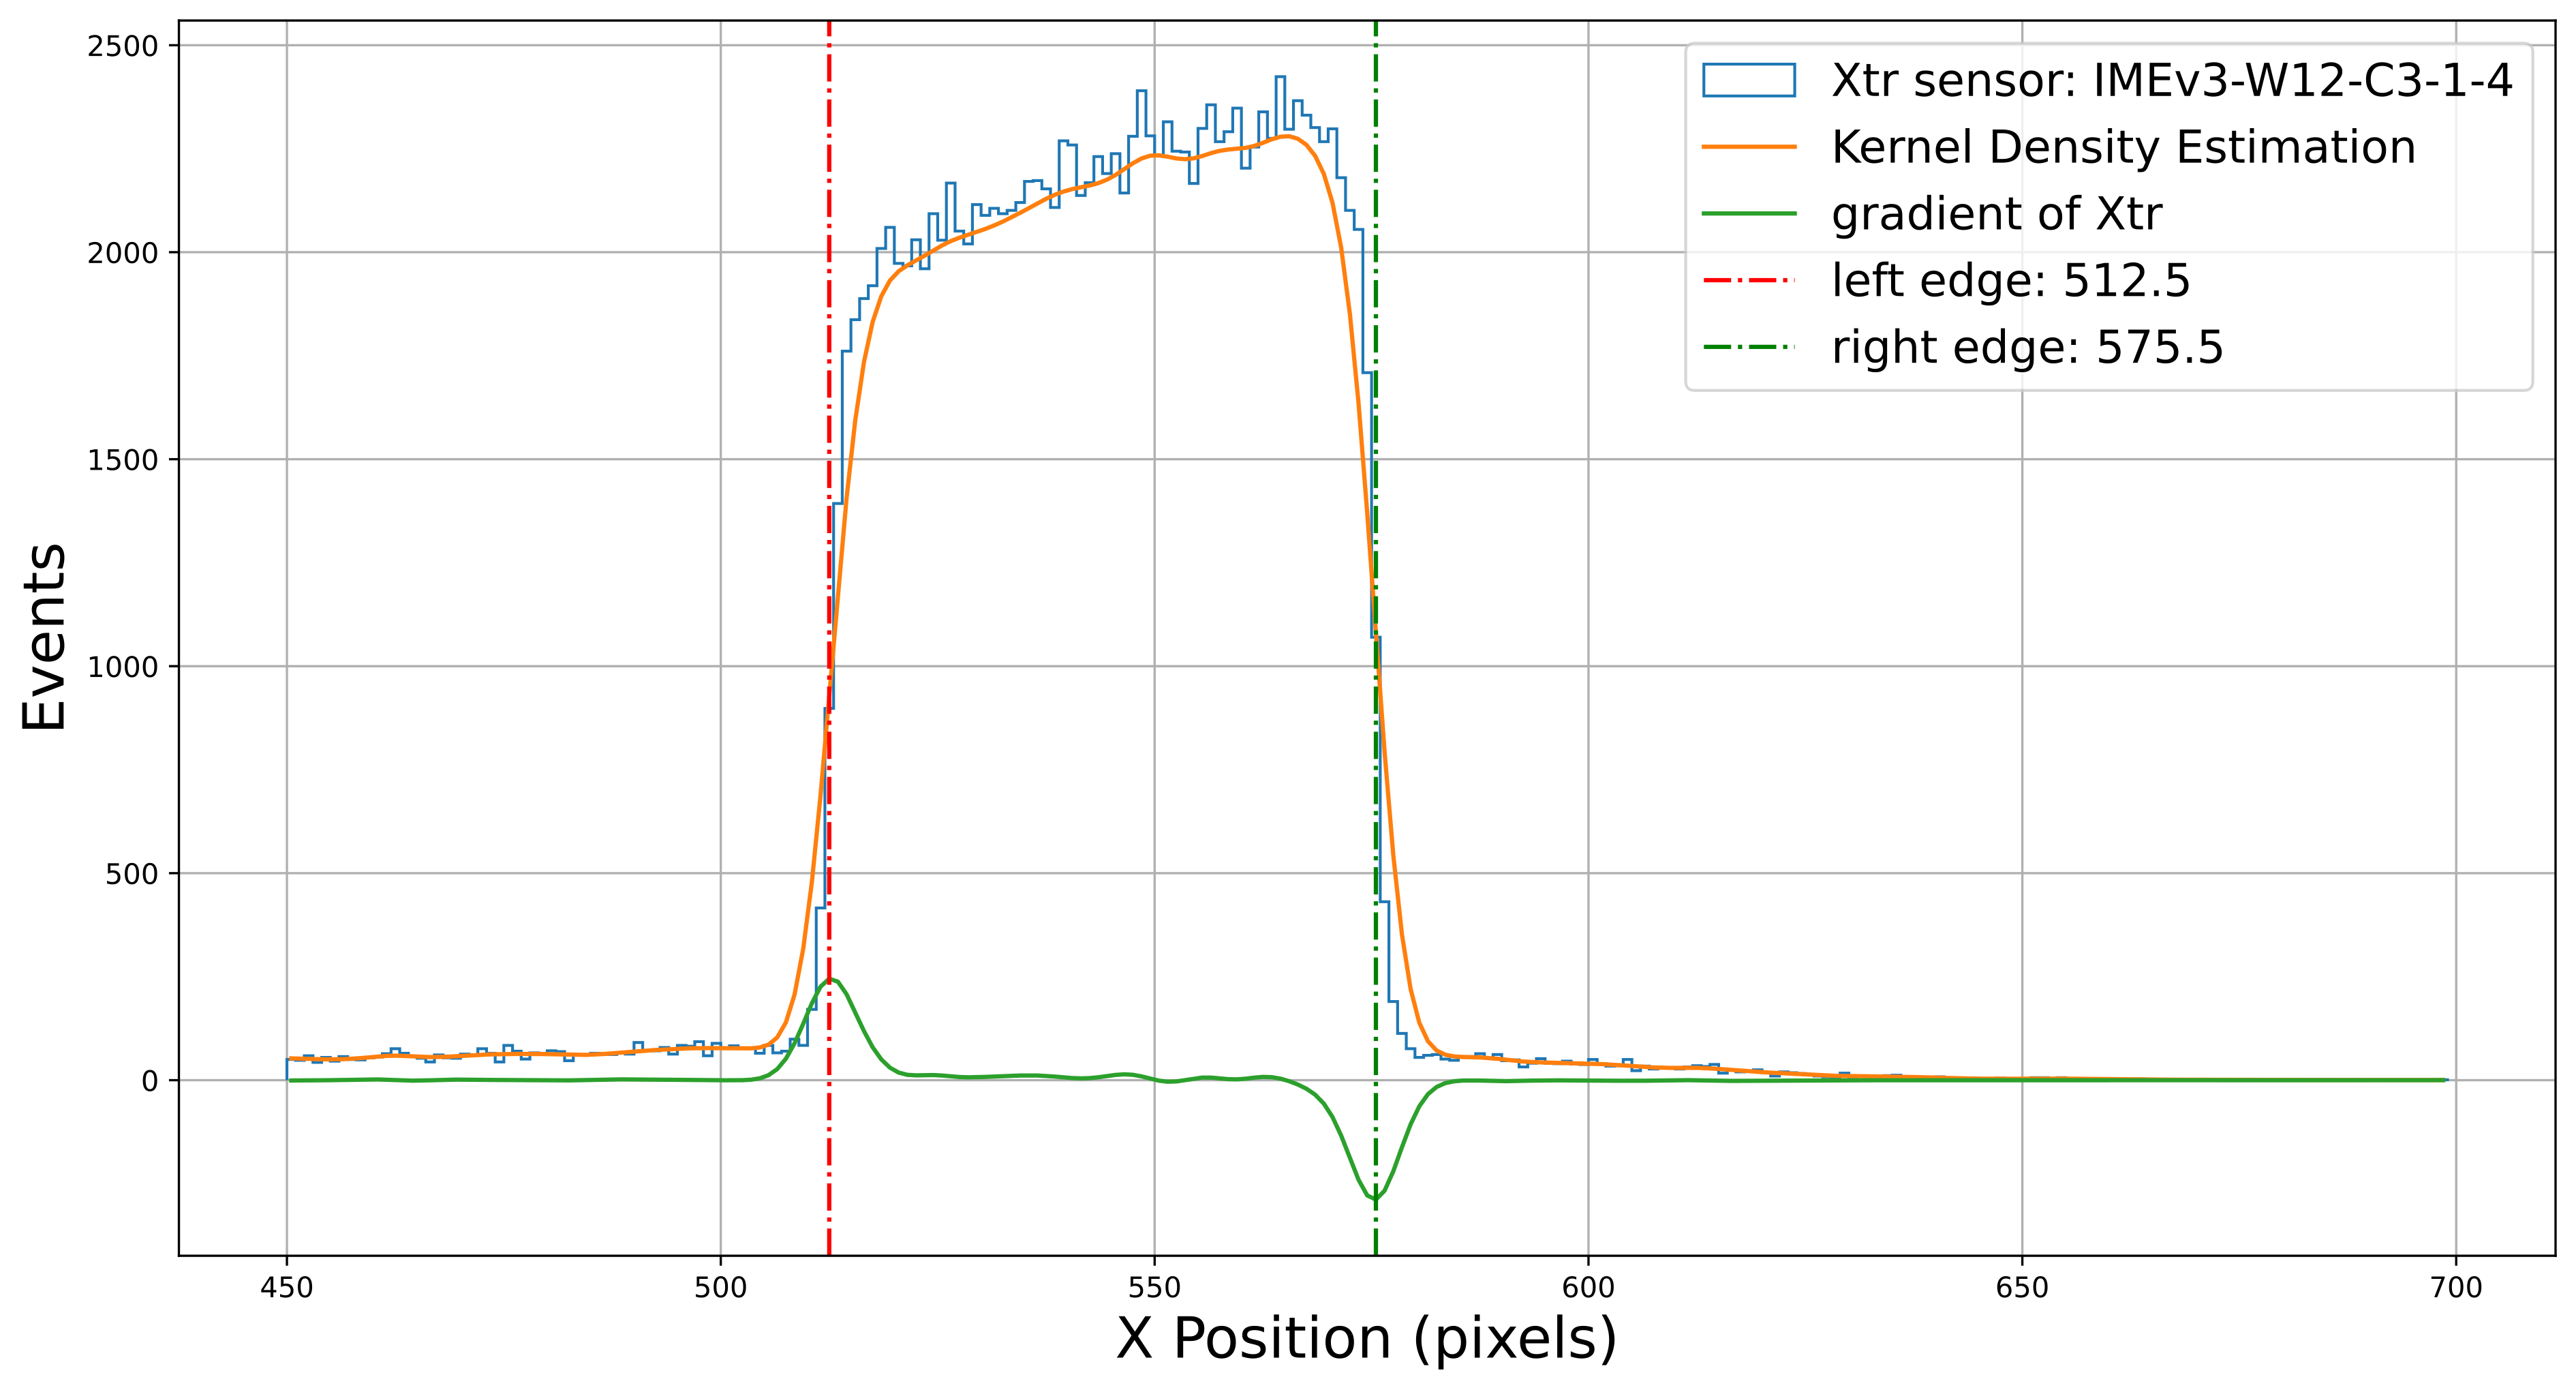
\includegraphics[width=.7\linewidth]{Images/methods/locating_edges_Xtr_batch_401_S1_DUT3.png}
    \captionsetup{width=\captionwidth}
    \caption{Projection of hits on the X axis after the \nameref{subsec:pulseHeight_cut}. By taking its derivative, it was possible to determine the position of the edges of the sensor. The unit is pixels of MIMOSA planes.}
    \label{fig:edges_of_the_sensor}
\end{figure}

Looking at the projections of hits on the X and Y coordinates, it was possible to determine the outline of the pad. The distribution was smoothed\footnote{Using a Kernel Density Estimator, as done previously for the pulse height distribution in Section \ref{subsec:pulseHeight_cut}} and its gradient (derivative) was calculated. This gave rise to two remarkably pronounced peaks shown in Figure~\ref{fig:edges_of_the_sensor}, which could be interpreted as the edges of the pads. By applying this procedure to both the X and Y projections we determined the horizontal and vertical edges, respectively. The final rectangular shape can be seen in Figure~\ref{fig:pulseHeight_cut_highlight}, alongside with the density of hits after applying a \textit{pulseHeight cut}. In few cases the sensors were slightly tilted in the XY plane, giving rise to slightly imprecise outlines, this is shown in Appendix, although it did not have a significant impact on the rest of the analysis.
%%% TODO: example of imprecise outlines

% NOTE: the edges defined like this are smaller than the real size of the pad (which is 1.3x1.3 mm\(^2\)) \cite{Agapopoulou_2022} \marginpar{\flushleft There is an outer guard ring isolating, so maybe the size is correct}

For certain properties that were analysed (such as efficiency and time resolution) it became clear that the rough selection of the contour of the pad was not always sufficient. Thus, an additional \textit{central area cut} was set up. A region of \(0.5\times0.5\si{mm^2}\) in the center of the pad was selected (similarly to what had been done in \cite{Agapopoulou_2022}) in order to avoid undesirable effects originating from the region outside the gain layer of the LGAD. (maybe details about LGADs guard ring and front view?)

\begin{figure}[h!tbp]
    \centering
    \subfloat[The heatmap of the reconstructed tracks without any cuts applied. The large rectangular shape is produced by the region of interest (ROI) selected with the FE-I4.]{
        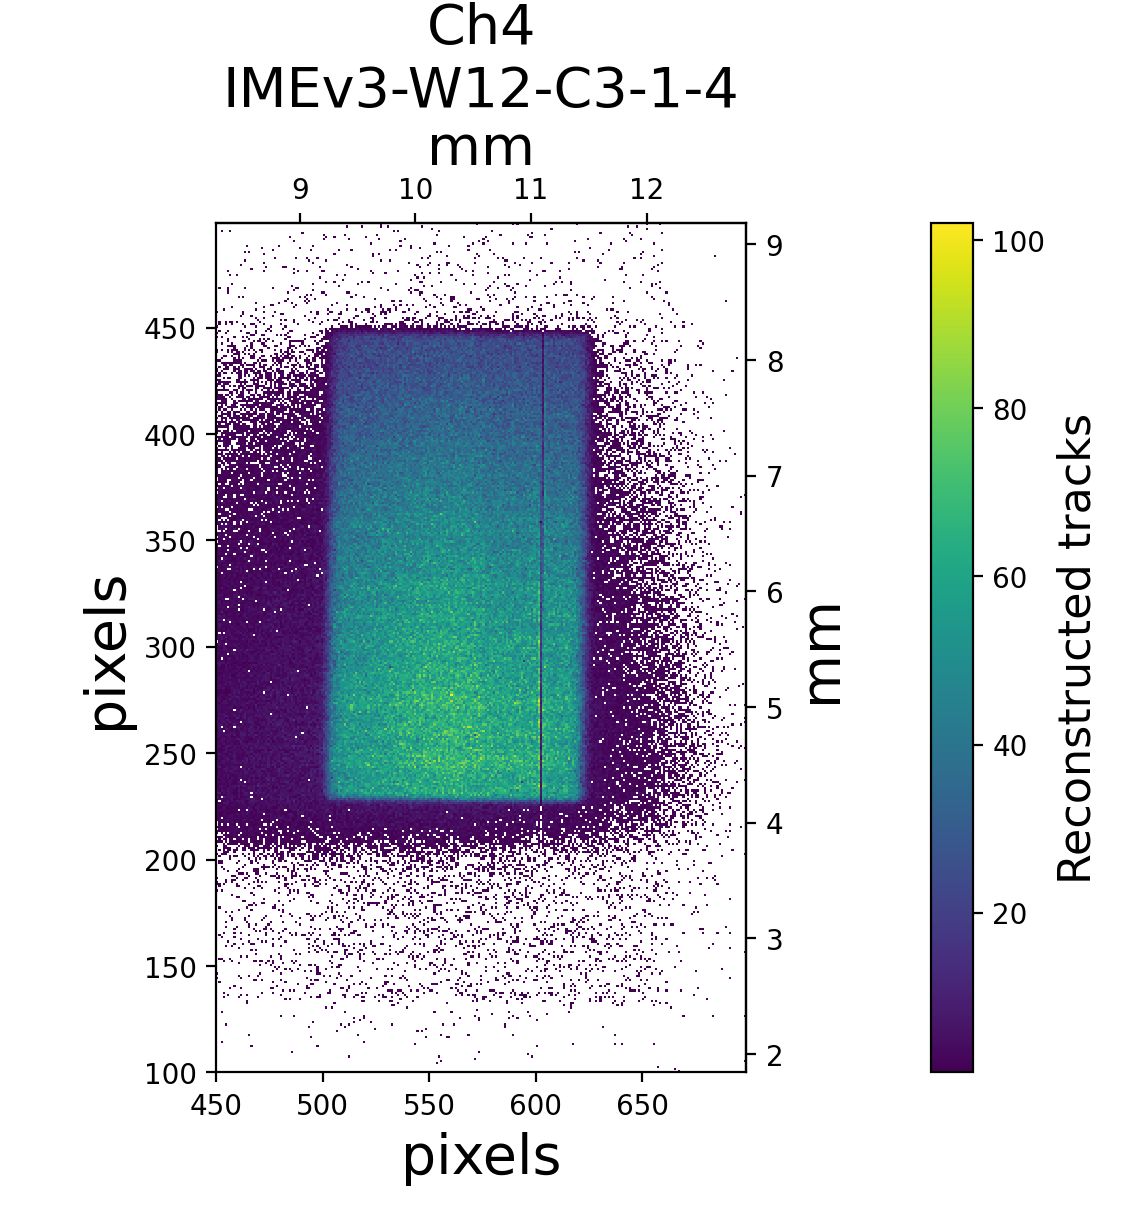
\includegraphics[width=.47\linewidth]{Images/methods/2D_Tracks_401 S1 (no cuts)_DUTs_3.png}
        \label{fig:hits_no_cuts}}
    \hfill
    \subfloat[The smaller rectangle corresponds to the area of the pad (highlighted in red with sides lengths) found by applying a \textit{pulseHeight cut}.]{
        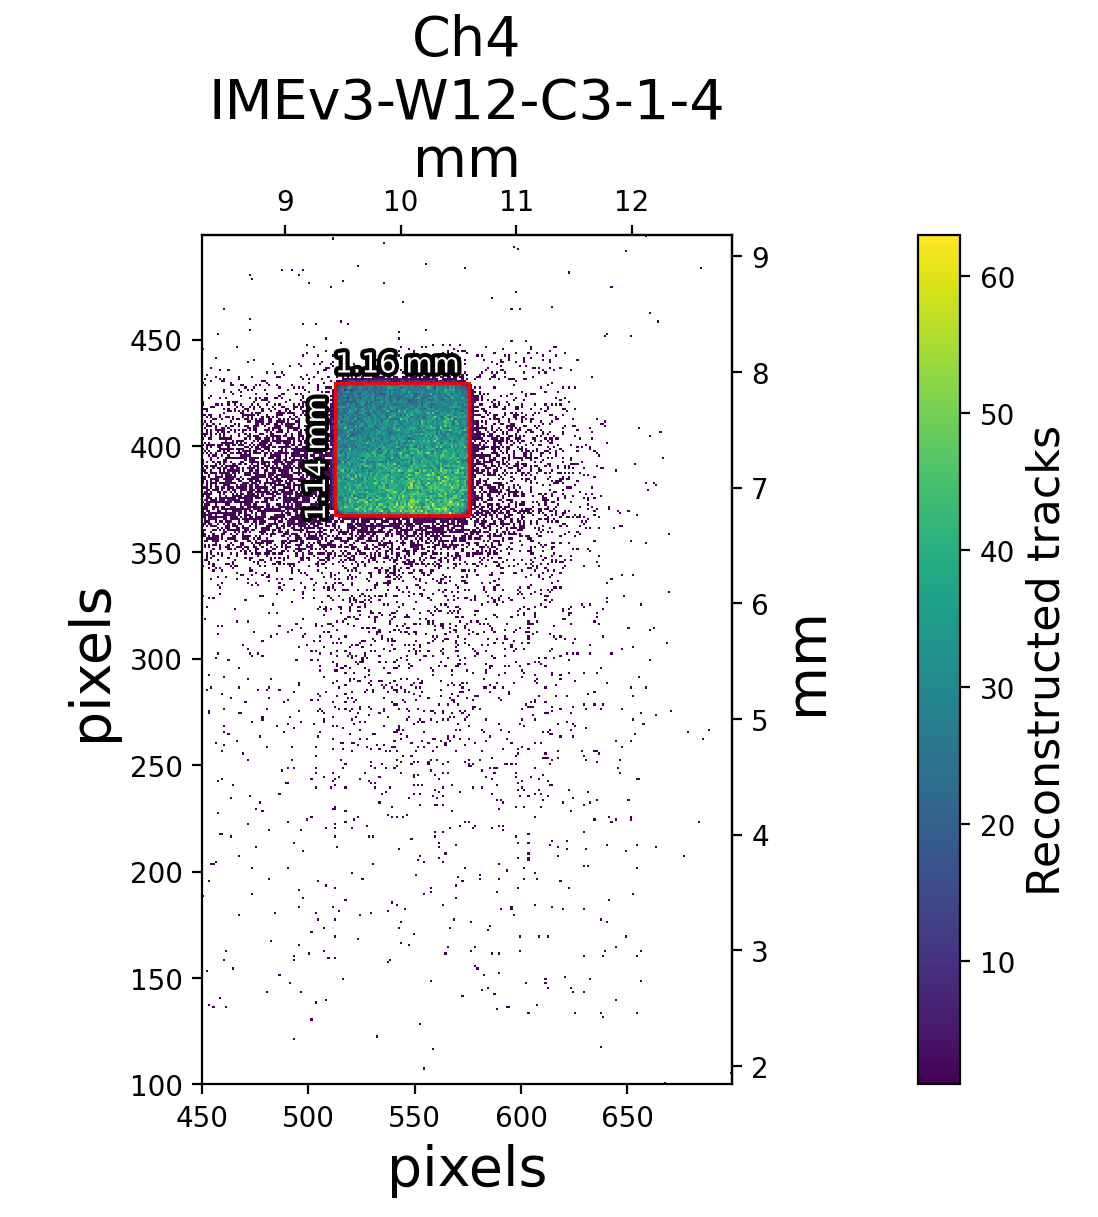
\includegraphics[width=.45\linewidth]{Images/methods/2D_Tracks_401_S1 highlight geometry cut (using pulseHeight).png}
        \label{fig:pulseHeight_cut_highlight}}
    \captionsetup{width=\captionwidth}
    \caption{later}
\end{figure}

\subsection{Time cut}\label{subsec:time_cut}

Additionally, to further clean the data, a cut on the \(\Delta t\) was applied.

Firstly the distribution of \(\Delta t\) (\(t_{DUT}-t_{MCP}\), time of arrival of the DUT - MCP) without any other cut was fit with a Gaussian plus a uniform background (Figure~\ref{fig:time_cut_gauss+bg_fit}):

\begin{figure}[h!tbp]
    \centering
    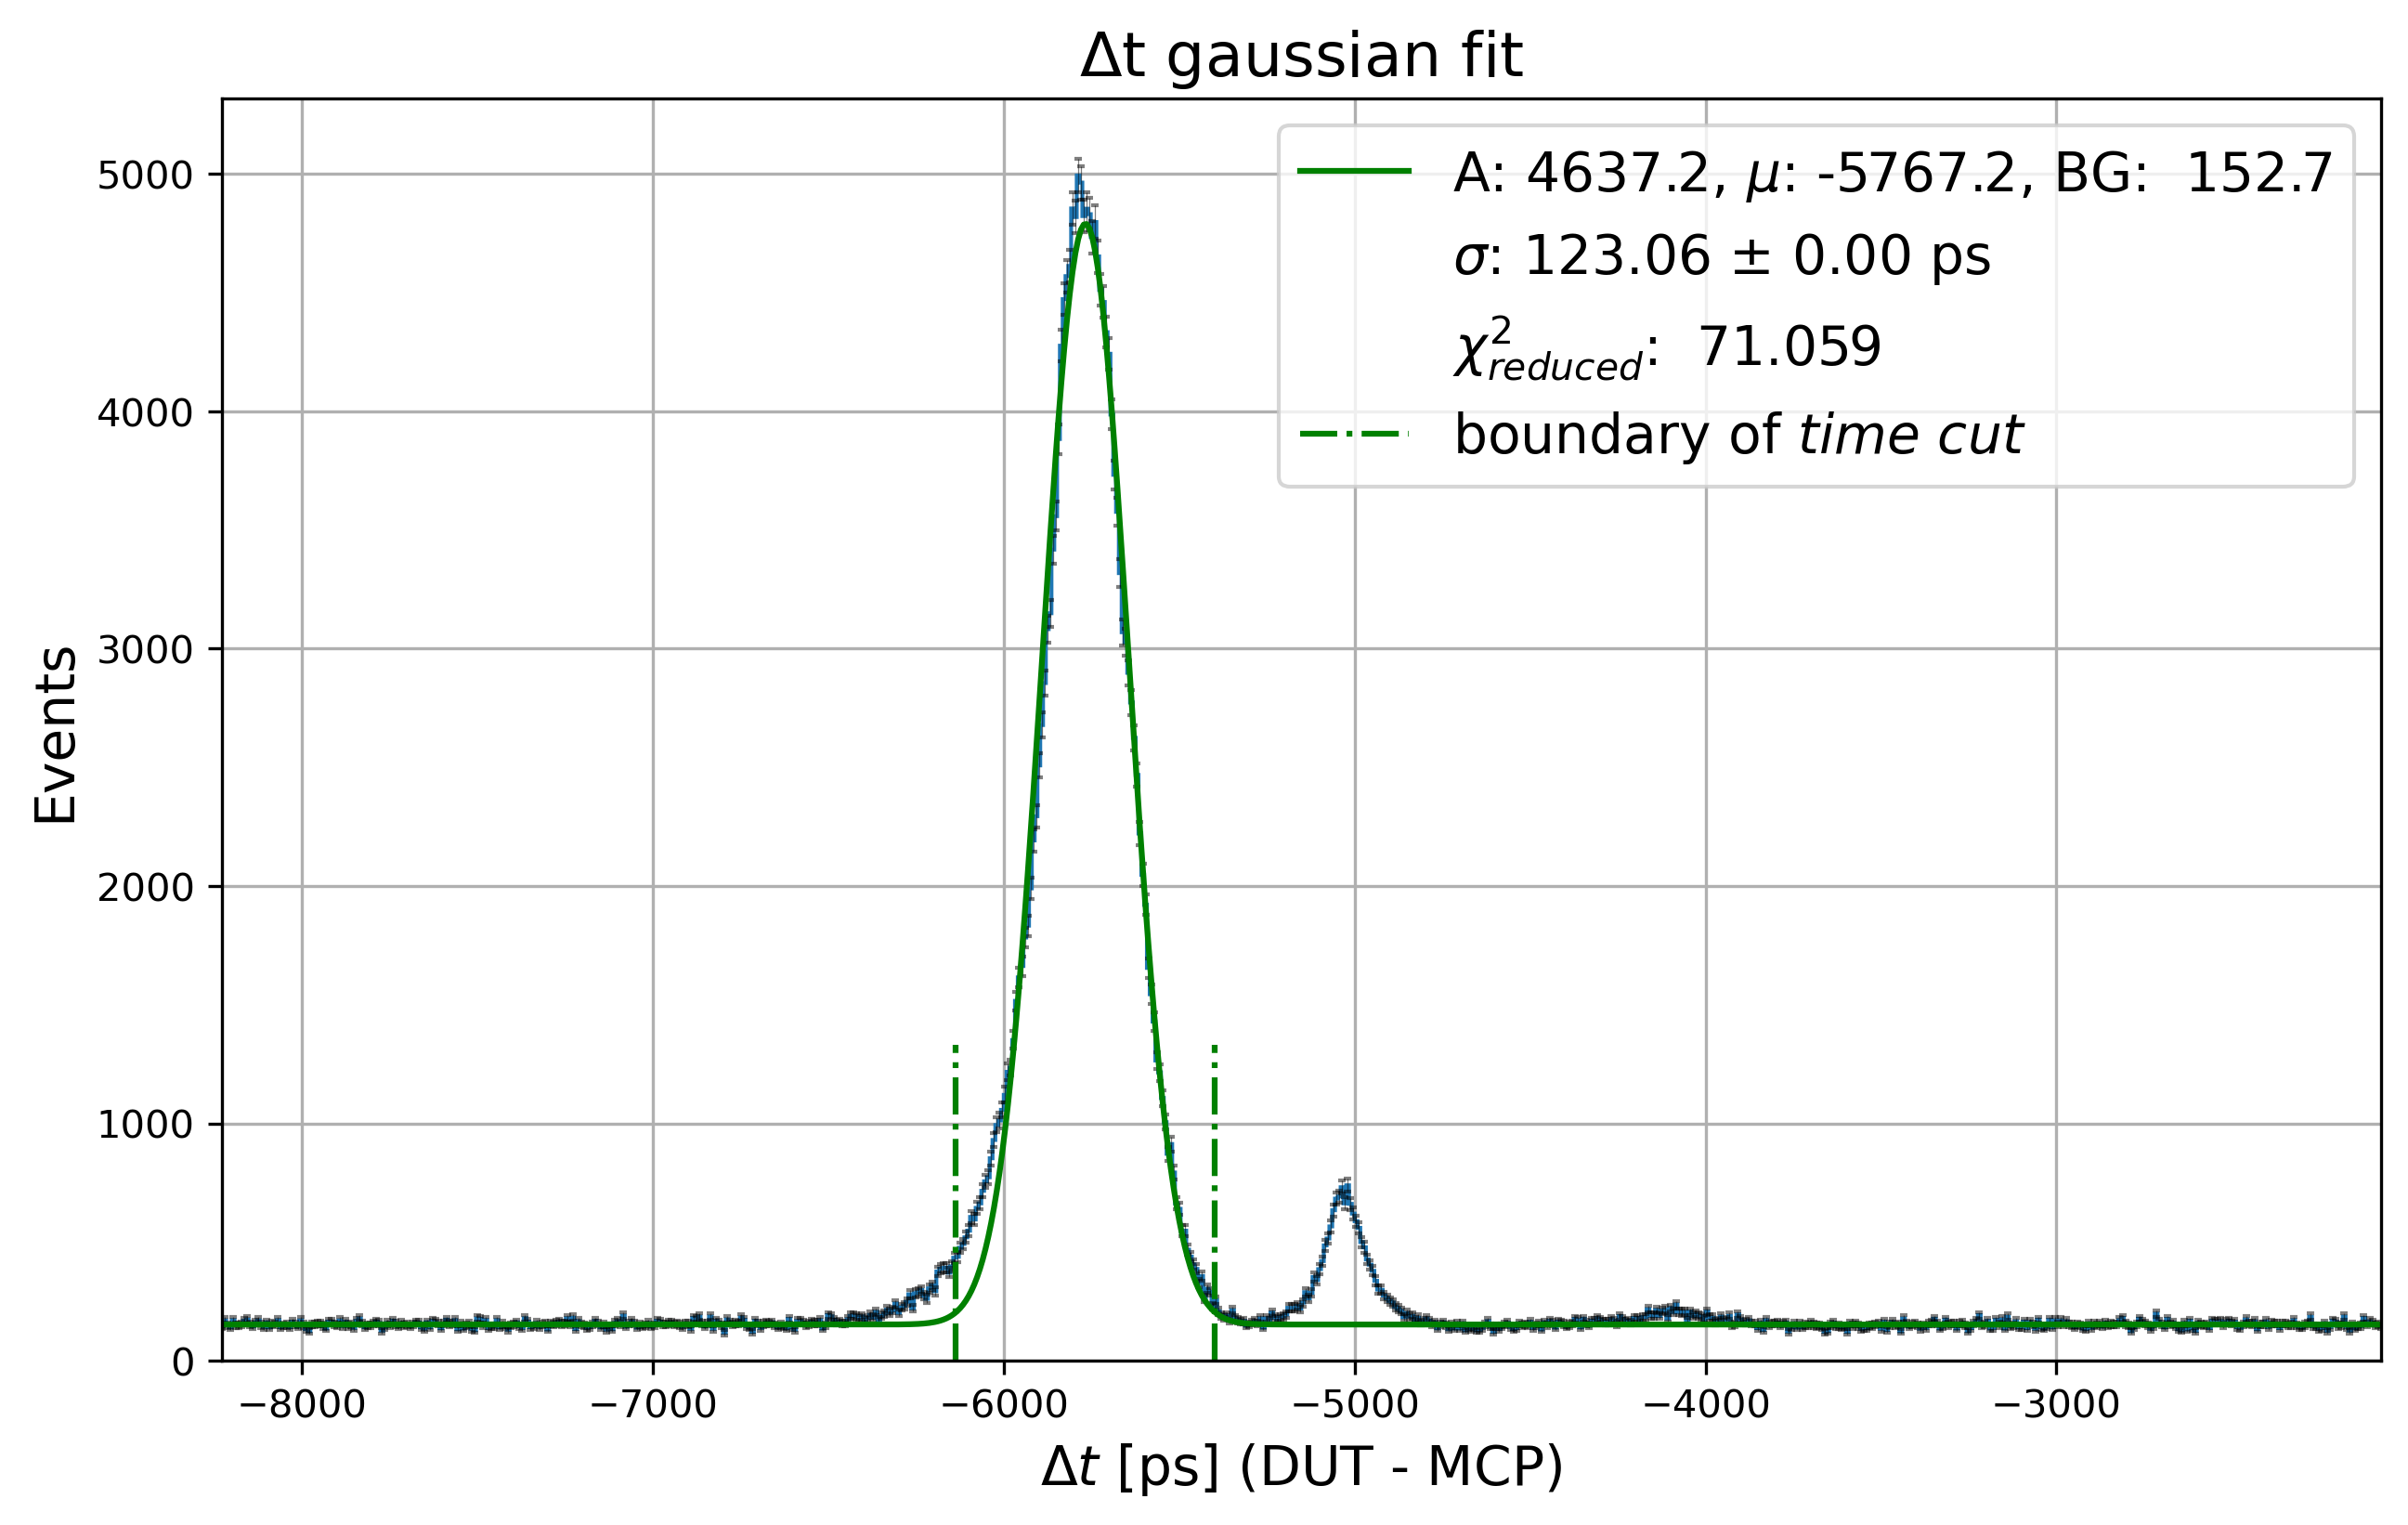
\includegraphics[width=.9\linewidth]{Images/methods/time_difference_603_S2_gauss_fit_no_cuts_DUT2.png}
    \captionsetup{width=\captionwidth}
    \caption{Time difference distribution (\(t_{DUT}-t_{MCP}\)) fit with a Gaussian + uniform background. The vertical dashed lines represent the boundary set as \textit{time cut}. The secondary peak 
     the right (i.e. delayed) is caused by a neighbouring pad, more detailed explanation in Section~\ref{sec:multiple_peaks}.}
    \label{fig:time_cut_gauss+bg_fit}
\end{figure}

\begin{equation*}
    f(x,A,\mu,\sigma,BG) = A \cdot e^{-\frac{1}{2}\left(\frac{x-\mu}{\sigma} \right)^2} + BG  \, .
\end{equation*}

\(A:\) Amplitude (n° of events);\quad \(\mu:\) Mean of the gaussian;\quad \(\sigma:\) Standard deviation;\quad \(BG:\) Uniform BackGround.

Ultimately, a \textit{time cut} was defined as all the events lying inside an interval of a number \(n\) of standard deviations \(\sigma\):

\begin{equation}
    (\mu-n\sigma;\mu+n\sigma) \, .
\end{equation}

Given that roughly 99.7\% of all values of a normal distribution lie within 3 standard deviations, \(n=3\) was deemed an adequate choice.

This cut proved to be especially useful in calculating the total efficiency of each pad and in fitting the charge distribution.

Some peculiarities became apparent, namely the second peak shifted to the right of the main one (meaning delayed compared to the latter) and some discrepancy with the expected Gaussian distribution around the left tail. These effects were further investigated and will be explained later in Sections \ref{sec:multiple_peaks} and \ref{sec:deviations_from_gaussian}.

\subsubsection{Heavily radiated sensor case}\label{subsec:geometry_cut_w/pulse_cut}

In some cases, typically for heavily radiated sensors, the noise in the pulse height distribution was too large (Figure~\ref{fig:pulseHeight_cut_failed}) to allow a \textit{pulseHeight cut} as in \ref{subsec:pulseHeight_cut}. This happened due to the pulse height decreasing and the noise peaks rising, so the separation between the two became less marked. In these situations it was possible to apply a \textit{time cut} instead and still get a satisfactory contour of the pad. The results between the two methods were very similar (Figure~\ref{fig:geometry_cut_comparison} in \nameref{chap:appendix}) so this seemed a good alternative.

\begin{figure}[ht]
    \centering
    \subfloat[Pulse height distribution, without a clear boundary between noise and signal.]{
        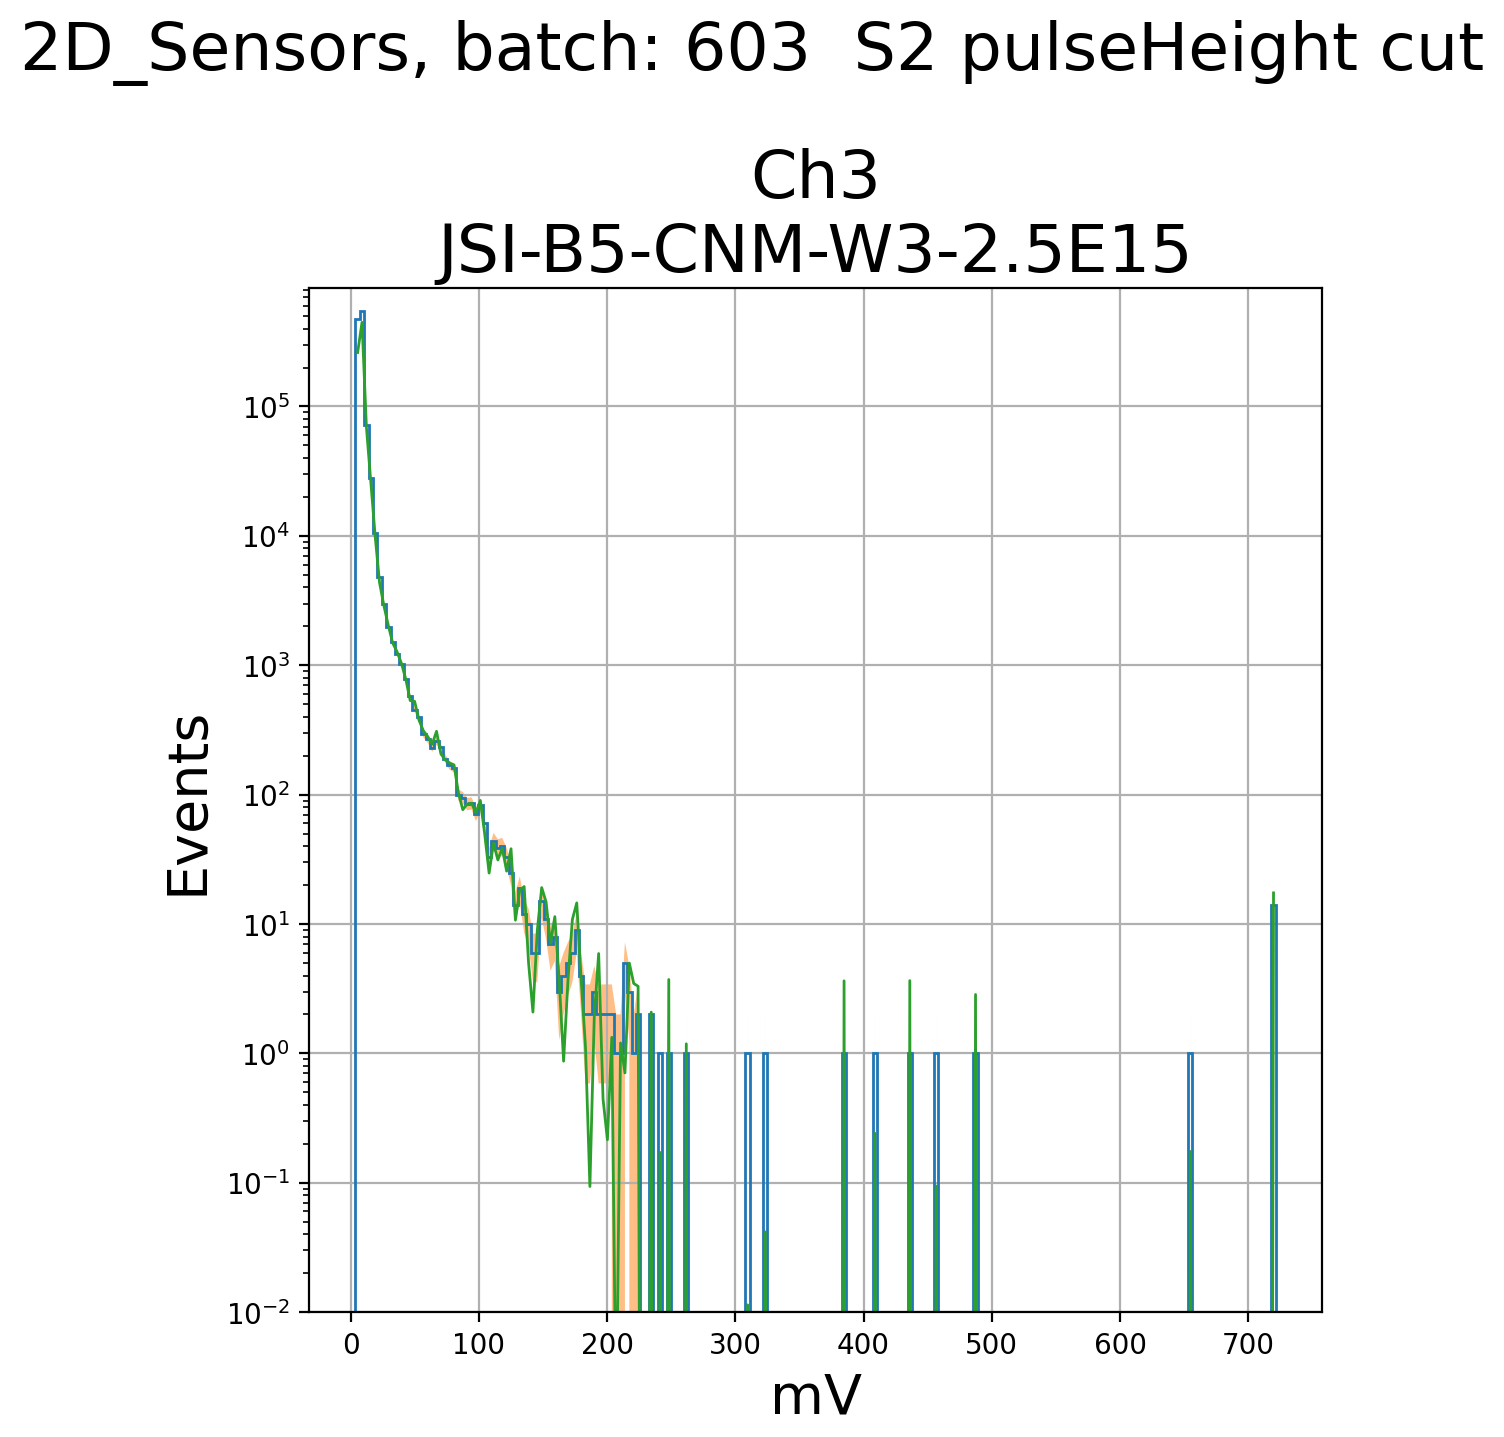
\includegraphics[width=.5\linewidth]{Images/methods/2D_Sensors_603 S2 pulseHeight cut_only_pulse.png}
        \label{fig:pulseHeight_cut_failed}}
    \hfill
    \centering
    \subfloat[Contour of the pad, highlighted in red, found by applying a time cut to the data. The irregular shape of the pad is caused by the ROI selected by the FEi4.]{
        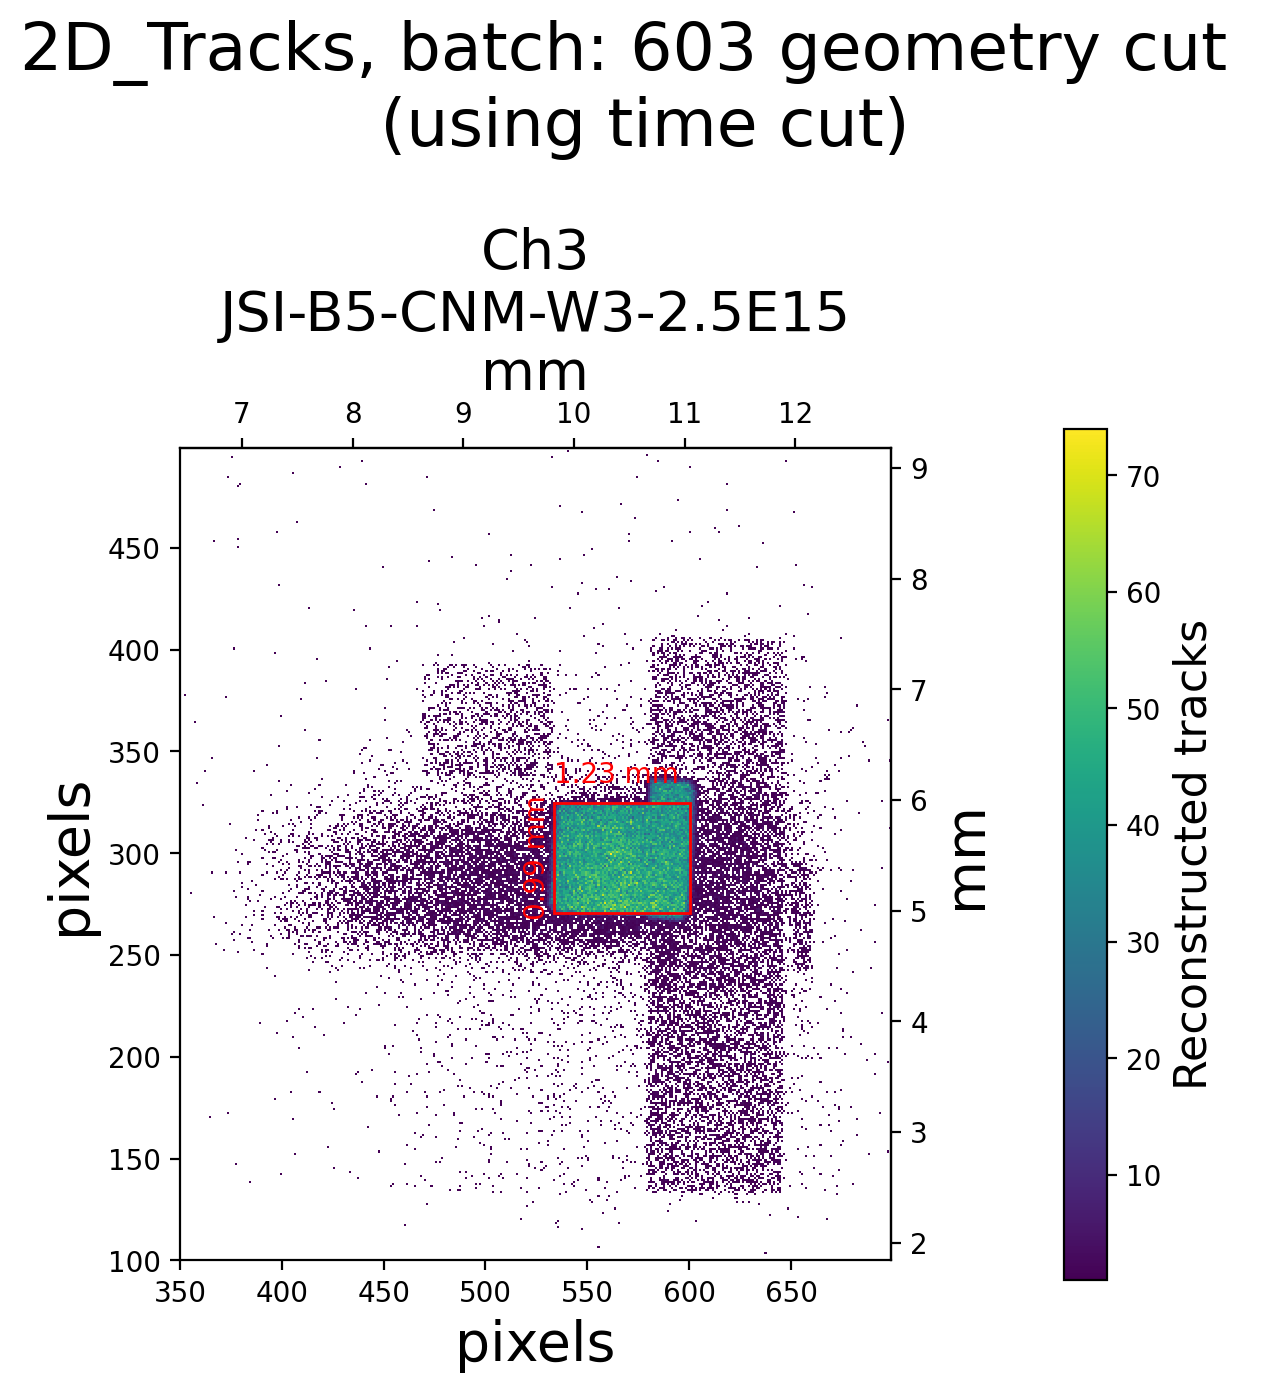
\includegraphics[width=.45\linewidth]{Images/methods/2D_Tracks_603_S2 highlight geometry cut (using time).png}
        \label{fig:time_cut_highlight}}
    \captionsetup{width=\captionwidth}
    \caption{Example of a different sensor (\textbf{irradiated}), for which the previous \textit{pulse height cut} became impractical (left), but using \textit{time cut} yielded a reasonable outline of the pad (right)}
\end{figure}

\subsection{Quality cuts validation}

To qualitatively confirm the soundness of the cuts performed, we plotted the density distribution of events of \(\boldsymbol{\Delta t}\) vs \textbf{pulse height} (Figures~\ref{fig:time_pulseHeight_nocut} and \ref{fig:time_pulseHeight_center}). The left plot shows all the available tracks, the right plot shows only the tracks that pass through the smaller central area of the DUT (a square of \(0.5\times0.5\si{mm^2}\) explained in Section~\ref{sec:geometry_cut}).

The plot on the right shows a narrow selection of events very likely to be a real signal (as they are guaranteed to have passed through the sensor). By comparing it with the plot on the left it can be noticed that a horizontal cut (\nameref{subsec:pulseHeight_cut}) and two vertical cuts (\nameref{subsec:time_cut}) provide indeed a good filter for physically meaningful events. 


\begin{figure}[h!tbp]
    \centering
    \subfloat[Density plot of all the event without any cuts applied. The red line and the green line show where \textit{pulse height cut} and \textit{time cut} would be applied, respectively.]{
        \includegraphics[width=.45\linewidth]{Images/methods/Time_pulseHeight_401_S1_with_info.png}
        \label{fig:time_pulseHeight_nocut}}
    \hfill
    \centering
    \subfloat[Density plot selecting only tracks passing through the central \(0.5\times0.5\si{mm^2}\) area of the pad.]{
        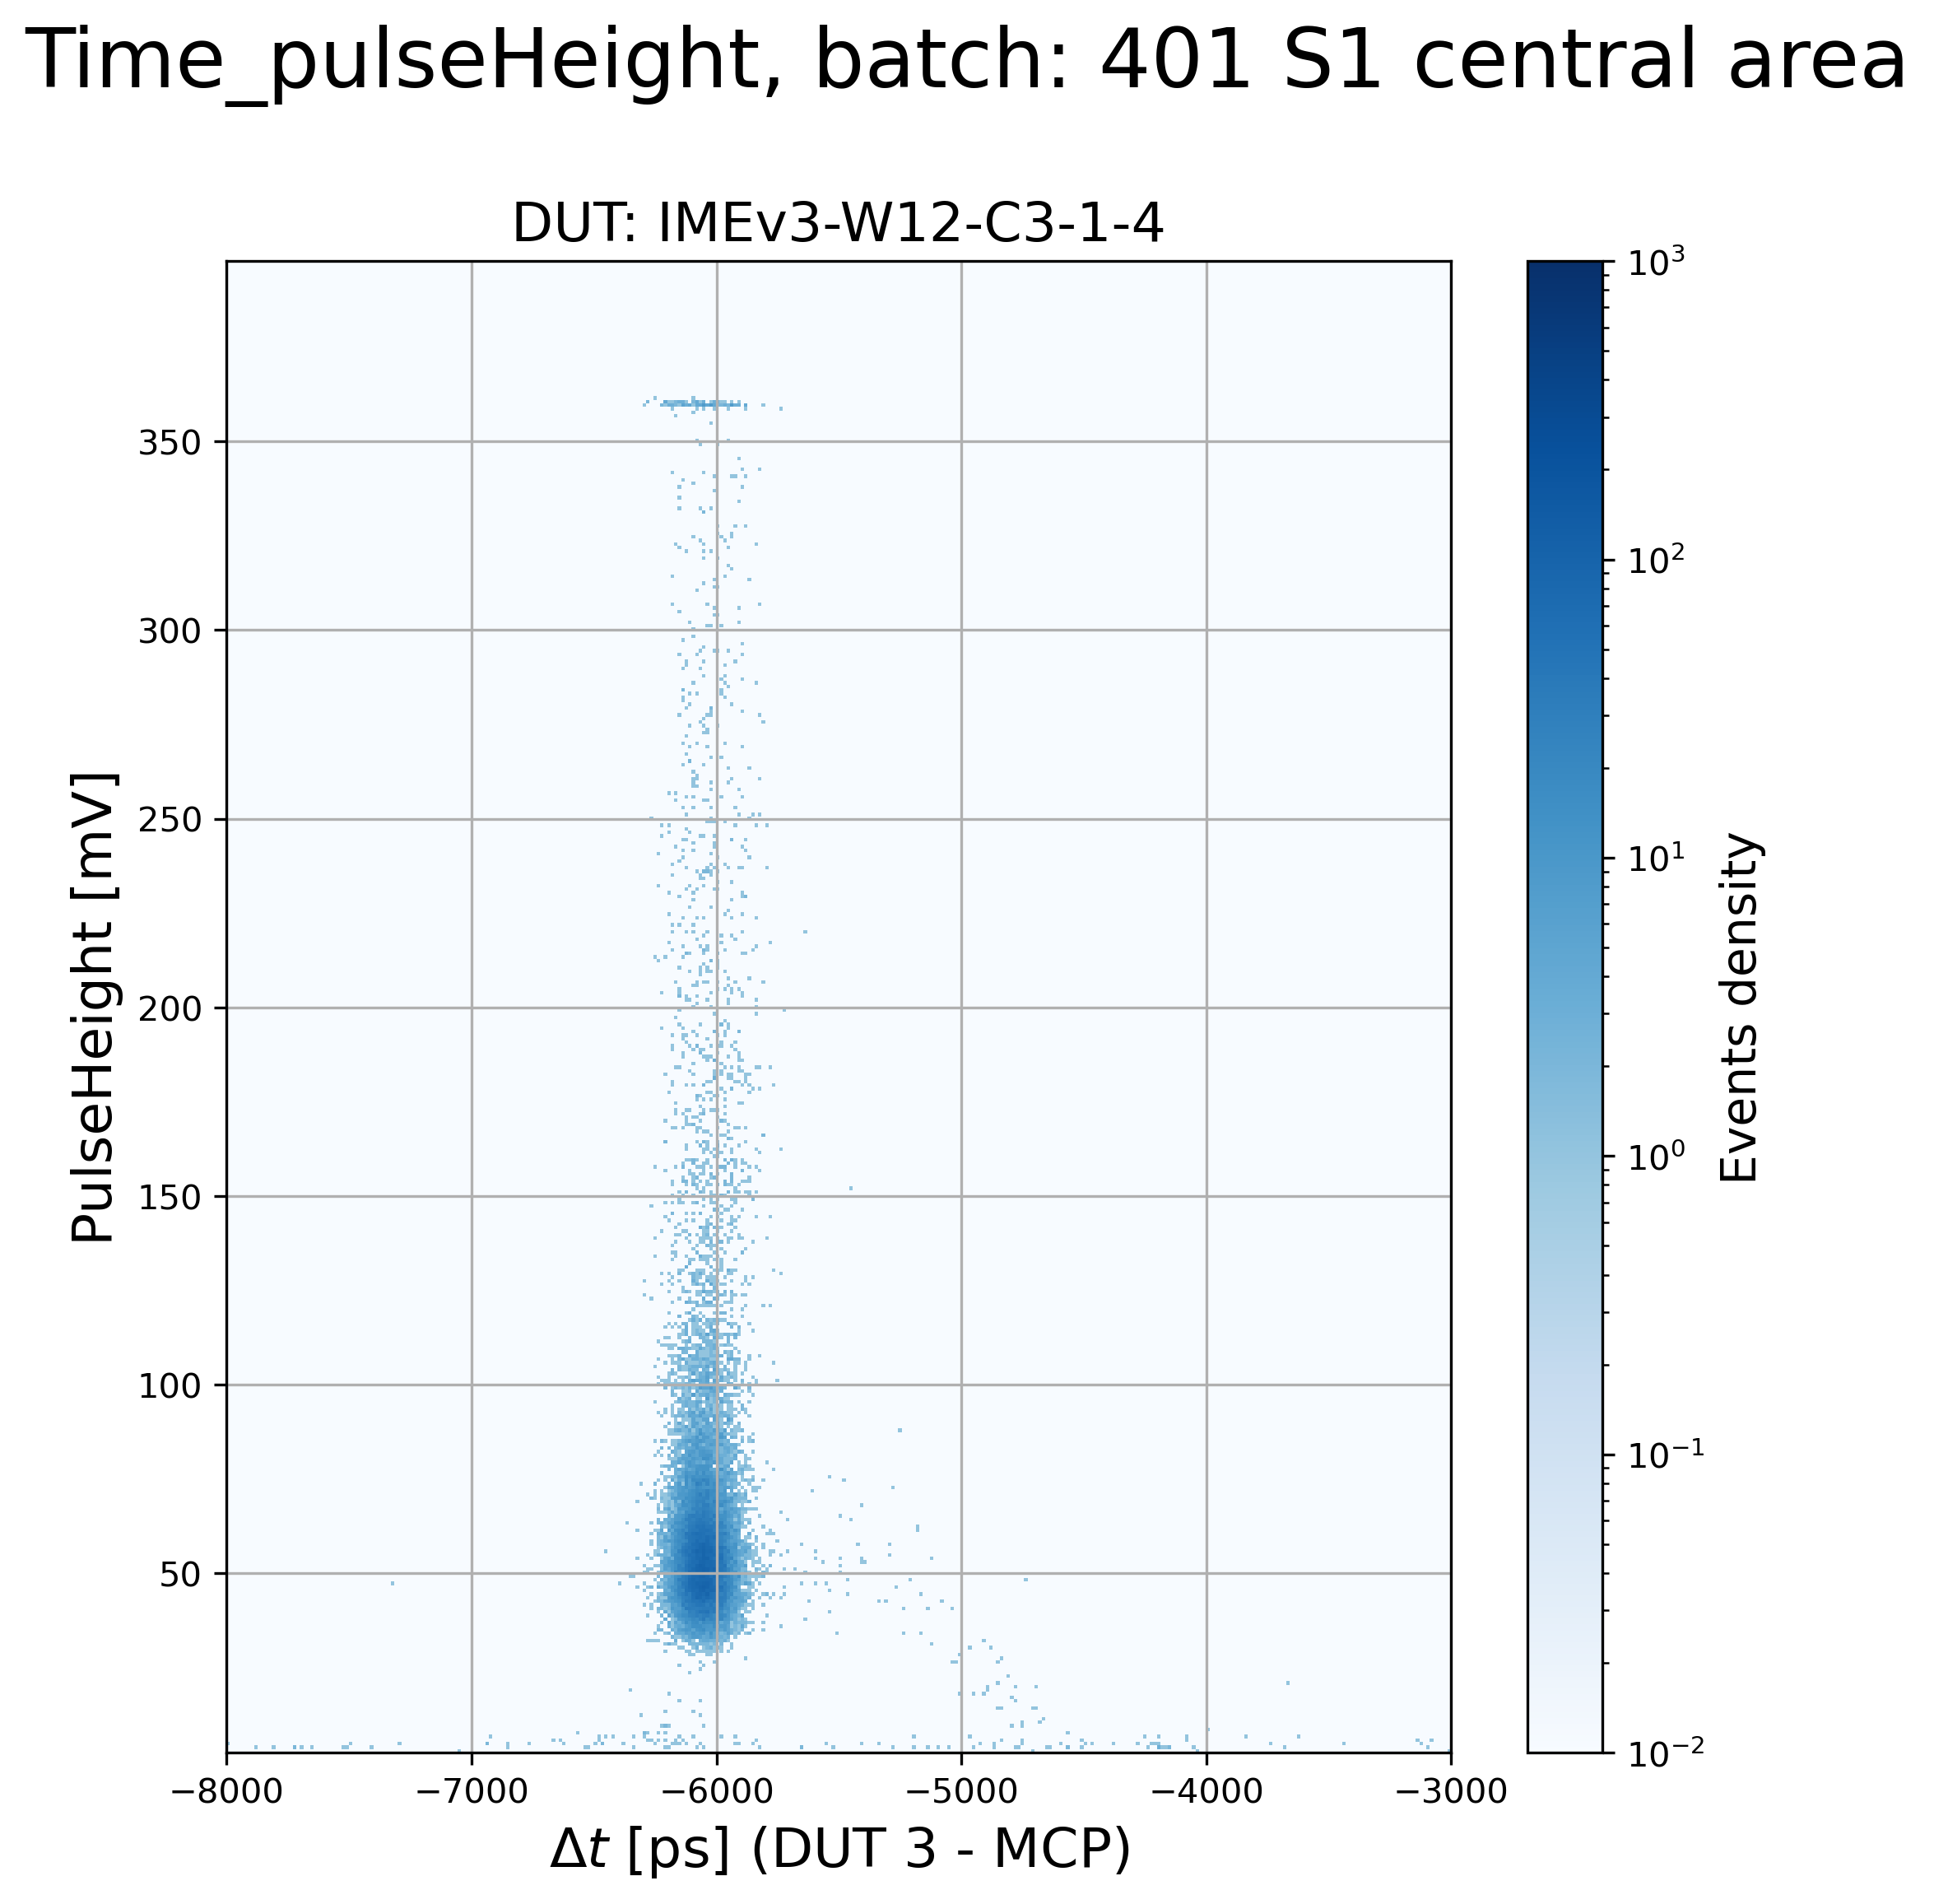
\includegraphics[width=.5\linewidth]{Images/methods/Time_pulseHeight_401S1 central area.png}
        \label{fig:time_pulseHeight_center}}
    \captionsetup{width=\captionwidth}
        \caption{Density plot of events when no cuts are applied (left) and when only a central square in the sensor is selected (right). The comparison between the two plots validates our choices made for quality cuts.}
\end{figure}


\section{Collected charge}\label{sec:methods_collected_charge}

A central goal of this study was to measure the distribution of the charge collected by the pads and verify their correspondence with the theoretical distribution: a convolution of a Gaussian and a Landau distribution (Appendix \ref{sec:vavilov_vs_landau_distribution}).

To achieve this, all the quality cuts defined in Section \ref{sec:qualtiy_cuts} were applied, and a fit was carried out using an implementation of the Gaussian*Landau convolution provided by the ROOT framework~\cite{Brun:1997pa} (Figure~\ref{fig:charge_ROOT_fit}).

The collected charge of a sensor is defined as the most probable value (MPV) of the charge, i.e. the highest point in the distribution.

\begin{figure}[h!tbp]
    \centering
    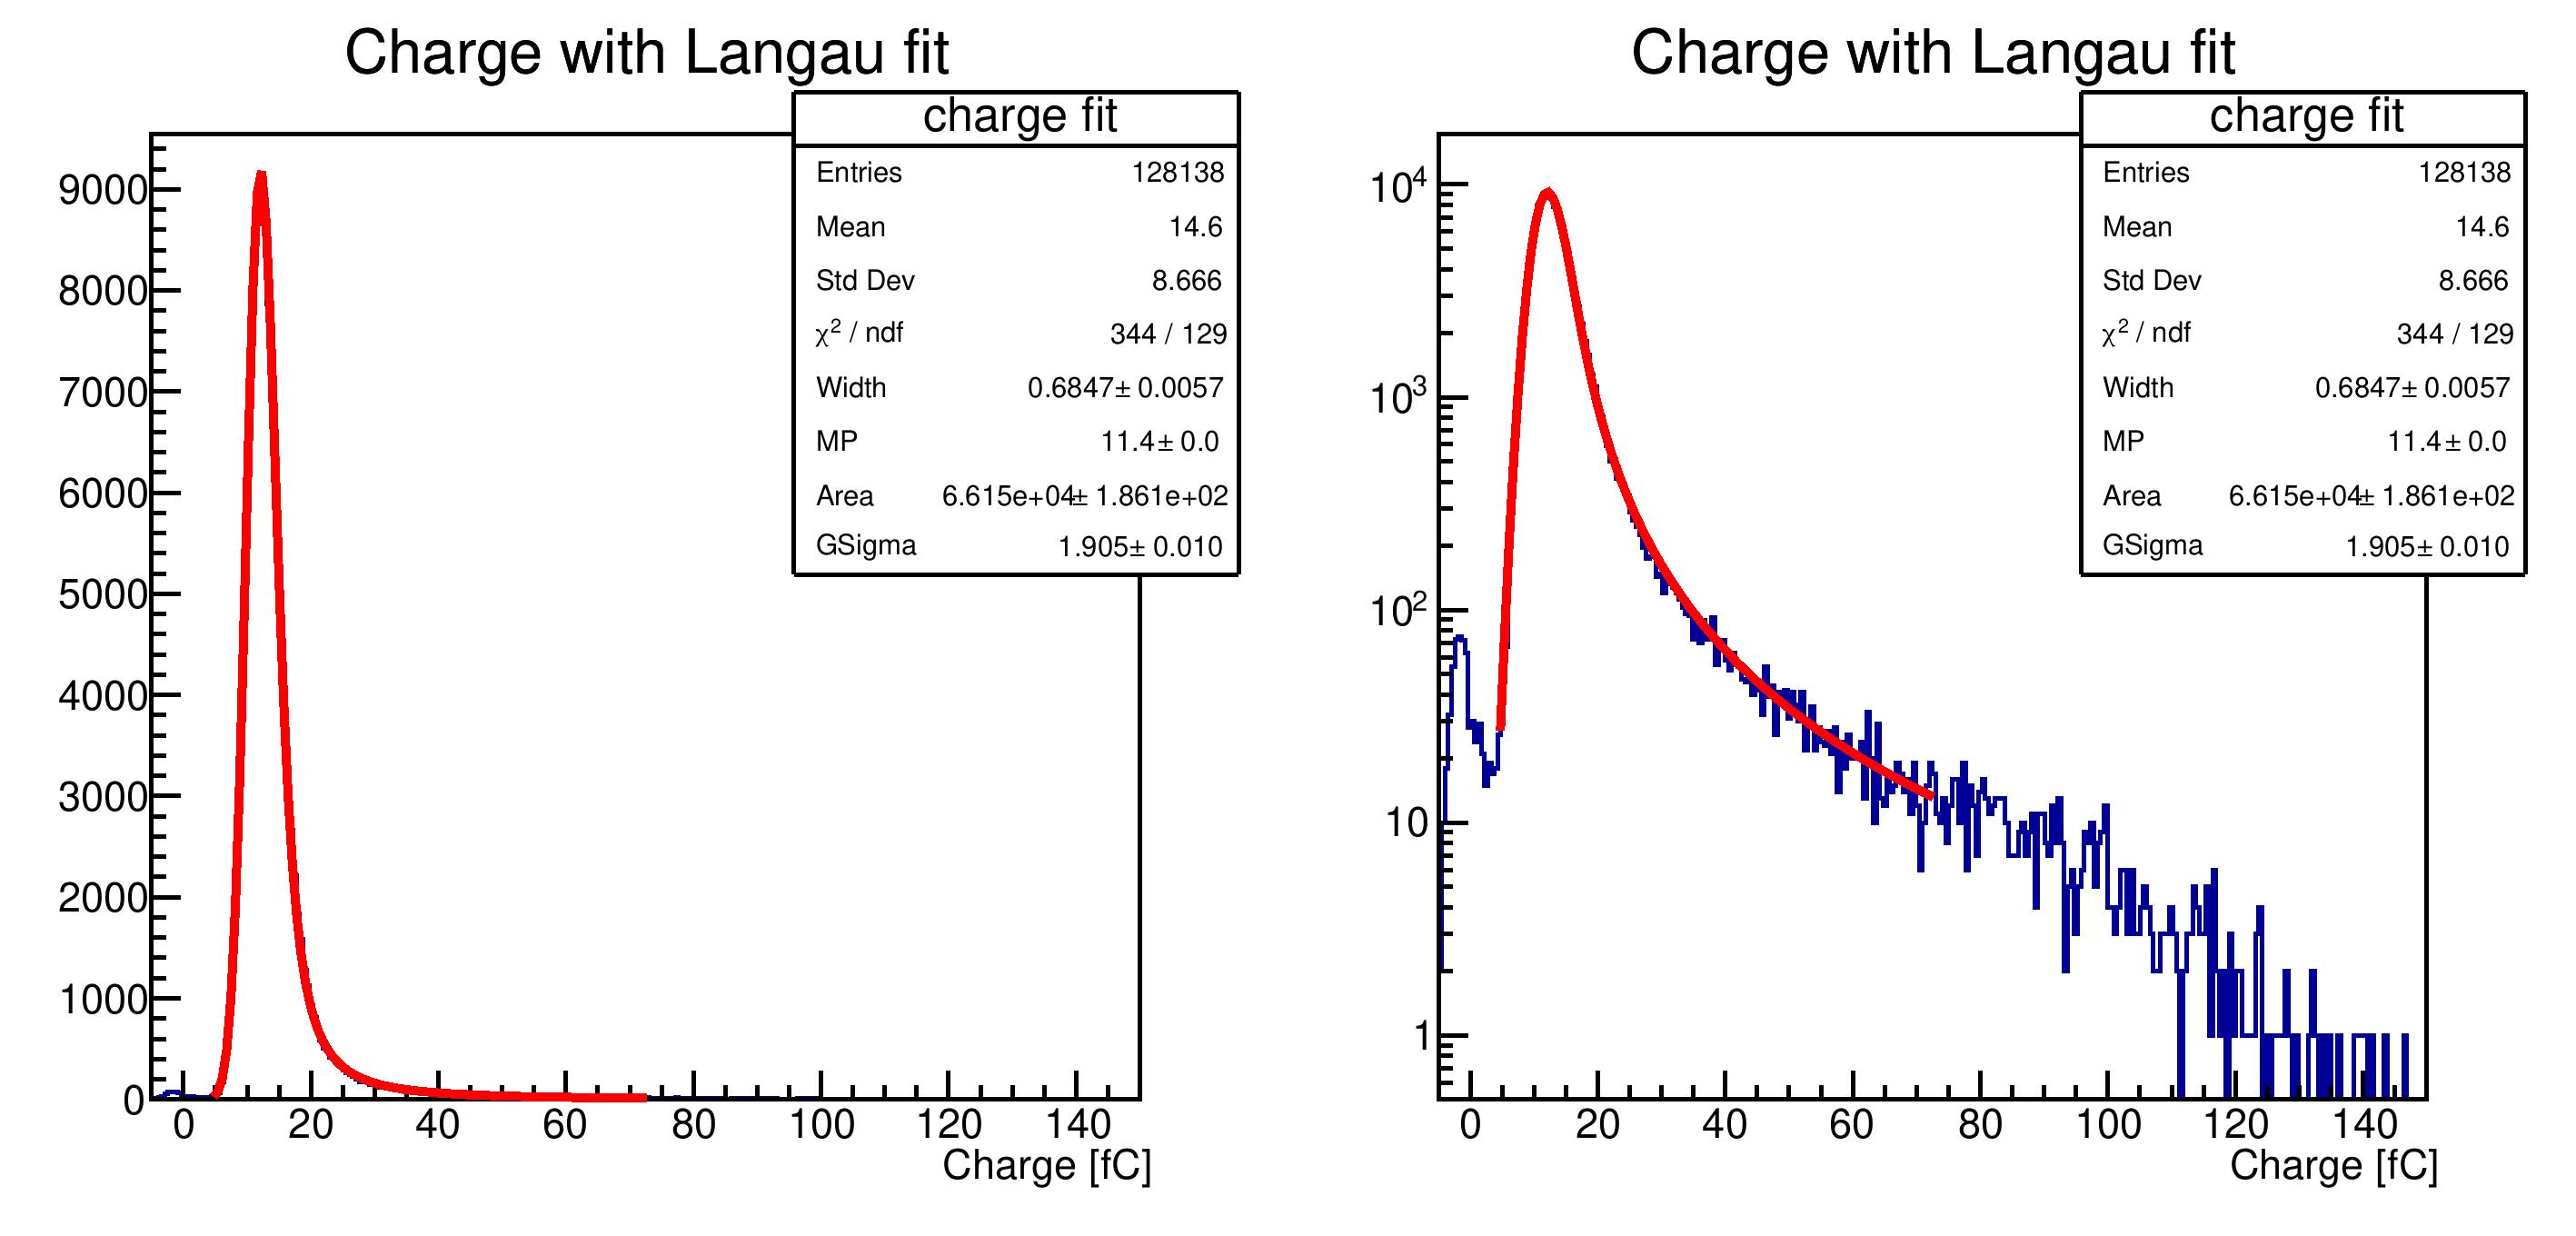
\includegraphics[width=1\linewidth]{Images/charge_plots/charge_data_all_cuts_401_S1_3_Charge_fit_ROOT_double_plot.png}
    \captionsetup{width=\captionwidth}
    \caption{Fit of the charge distribution (red) carried out with ROOT. On the right it is shown the same plot in logarithmic scale, to highlight the extra noise at \(\approx 0\).}
    \label{fig:charge_ROOT_fit}
\end{figure}

\subsubsection{Gain}
% charged particle in 50 um of silicon produce ~0.52 fC of charge or 3280 e-h pairs
The gain is obtained by dividing the most probable value of the collected charge by the expected charge from a minimum ionizing particle (MIP) in a silicon sensor without gain. For a \qty{50}{\micro\meter} thick sensor, this value is \(3280\) e-h pairs, equivalent to \qty{.52}{\femto\coulomb} \cite{meroli_energy_loss2011}.

\subsubsection{Extra noise}
Despite all the trimming to the data, a noticeable part of the noise centered at \(\approx 0\) could not be removed. We could not pinpoint the origin of this extra noise, but a lot of factors could contribute to it: track reconstruction, other electronic noise etc.
Considering this point, the fit was performed in a smaller interval, avoiding the noise (Figure~\ref{fig:charge_ROOT_fit}). The left limit was fixed at \(4\si{fC}\), as this is also the lowest signal that the electronic board is able to measure, the right limit was adjusted to include only bins with significant amount of data (and account for the \nameref{subsec:tail_discrepancies}, described in Appendix).

%%% maybe I can put a table to show which cuts I applied to which variables


\section{Efficiency}\label{sec:methods_efficiency}

The efficiency (\(\epsilon\)) was defined as the total number of tracks with charge larger than a certain \textit{threshold charge} divided by the total number of reconstructed track (\textbf{after} quality cuts had been applied).

% \begin{equation*}
%     \text{Efficiency} = \frac{\text{Tracks with } q>Q_{threshold}}{\text{Total tracks}}  \, .
% \end{equation*}

\begin{equation*}
    \epsilon = \frac{\text{Tracks with } q>Q_{threshold}}{\text{Total tracks}}  \, .
\end{equation*}

The threshold charge \(Q_{threshold}\) was chosen to be \(4\si{fC}\), which corresponds to the limit of sensitivity of the ASIC.

Before measuring the overall efficiency of the sensors, we applied a \textit{time cut} (as described in \nameref{subsec:time_cut}). Additionally, we elected to restrict the calculation to the smaller \textit{central area} of \(0.5\times0.5\si{mm^2}\) defined earlier in \nameref{sec:geometry_cut}. This area can be seen highlighted in red in Figure~\ref{fig:efficiency_2D_plot}, which also shows how the efficiency value computed for each individual squared binning of the surface.

Finally, the total efficiency was computed with different values of \textit{threshold charge} to obtain the plot in Figure~\ref{fig:efficiency_depending_threshold}, which shows that (in this example) the value remains constant well after the chosen threshold of \(4\si{fC}\).

\begin{figure}[h!tbp]
    \centering
    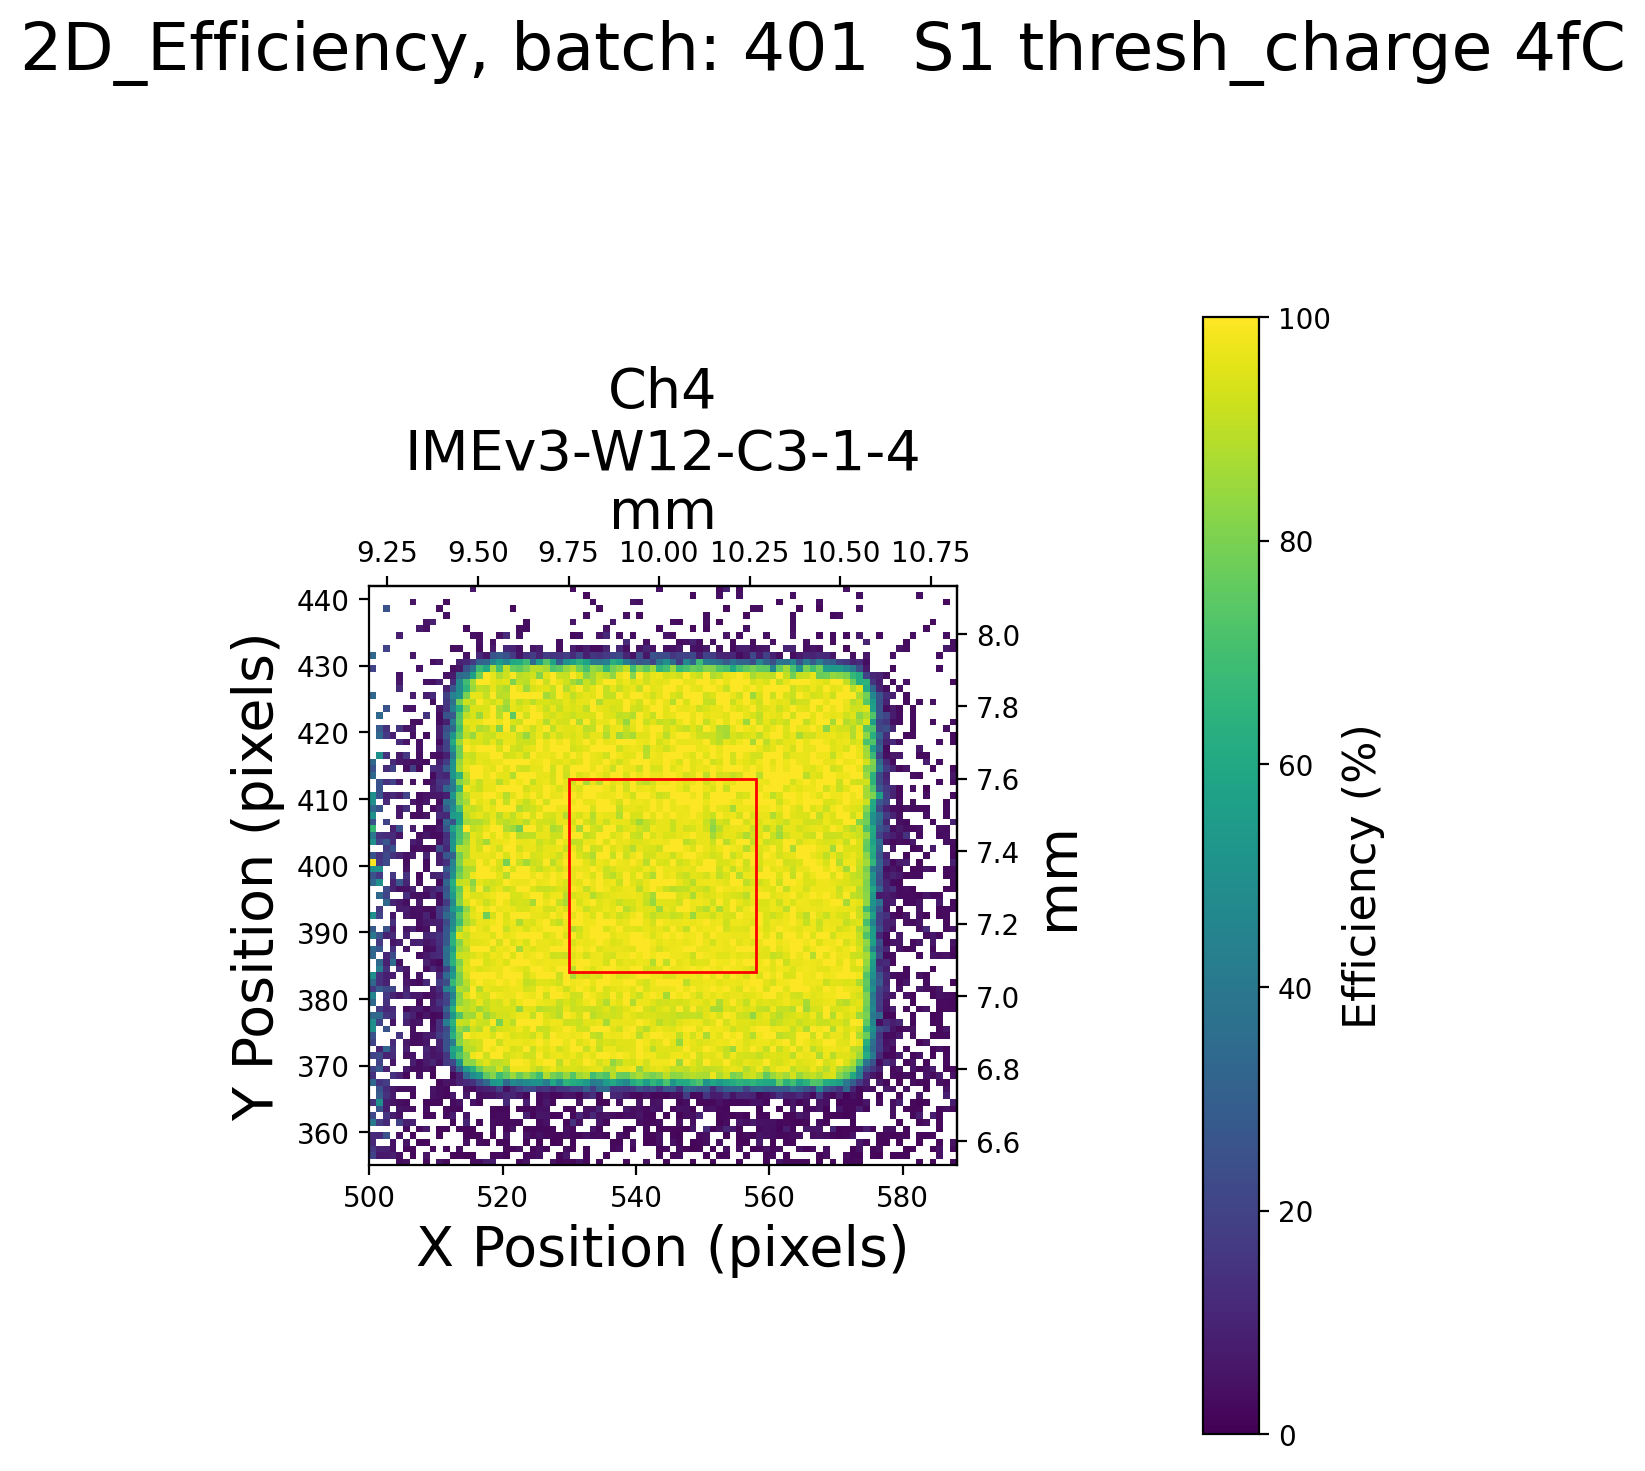
\includegraphics[width=0.7\linewidth]{Images/efficiency_plots/2D Efficiency_401_S1_with_center_highlight_DUTs_3.png}
    \captionsetup{width=\captionwidth}
    \caption{2D histogram plot of efficiency (per squared bin) and \textit{central area cut} highlighted in red.}
    \label{fig:efficiency_2D_plot}
\end{figure}

\begin{figure}[h!tbp]
    \centering
    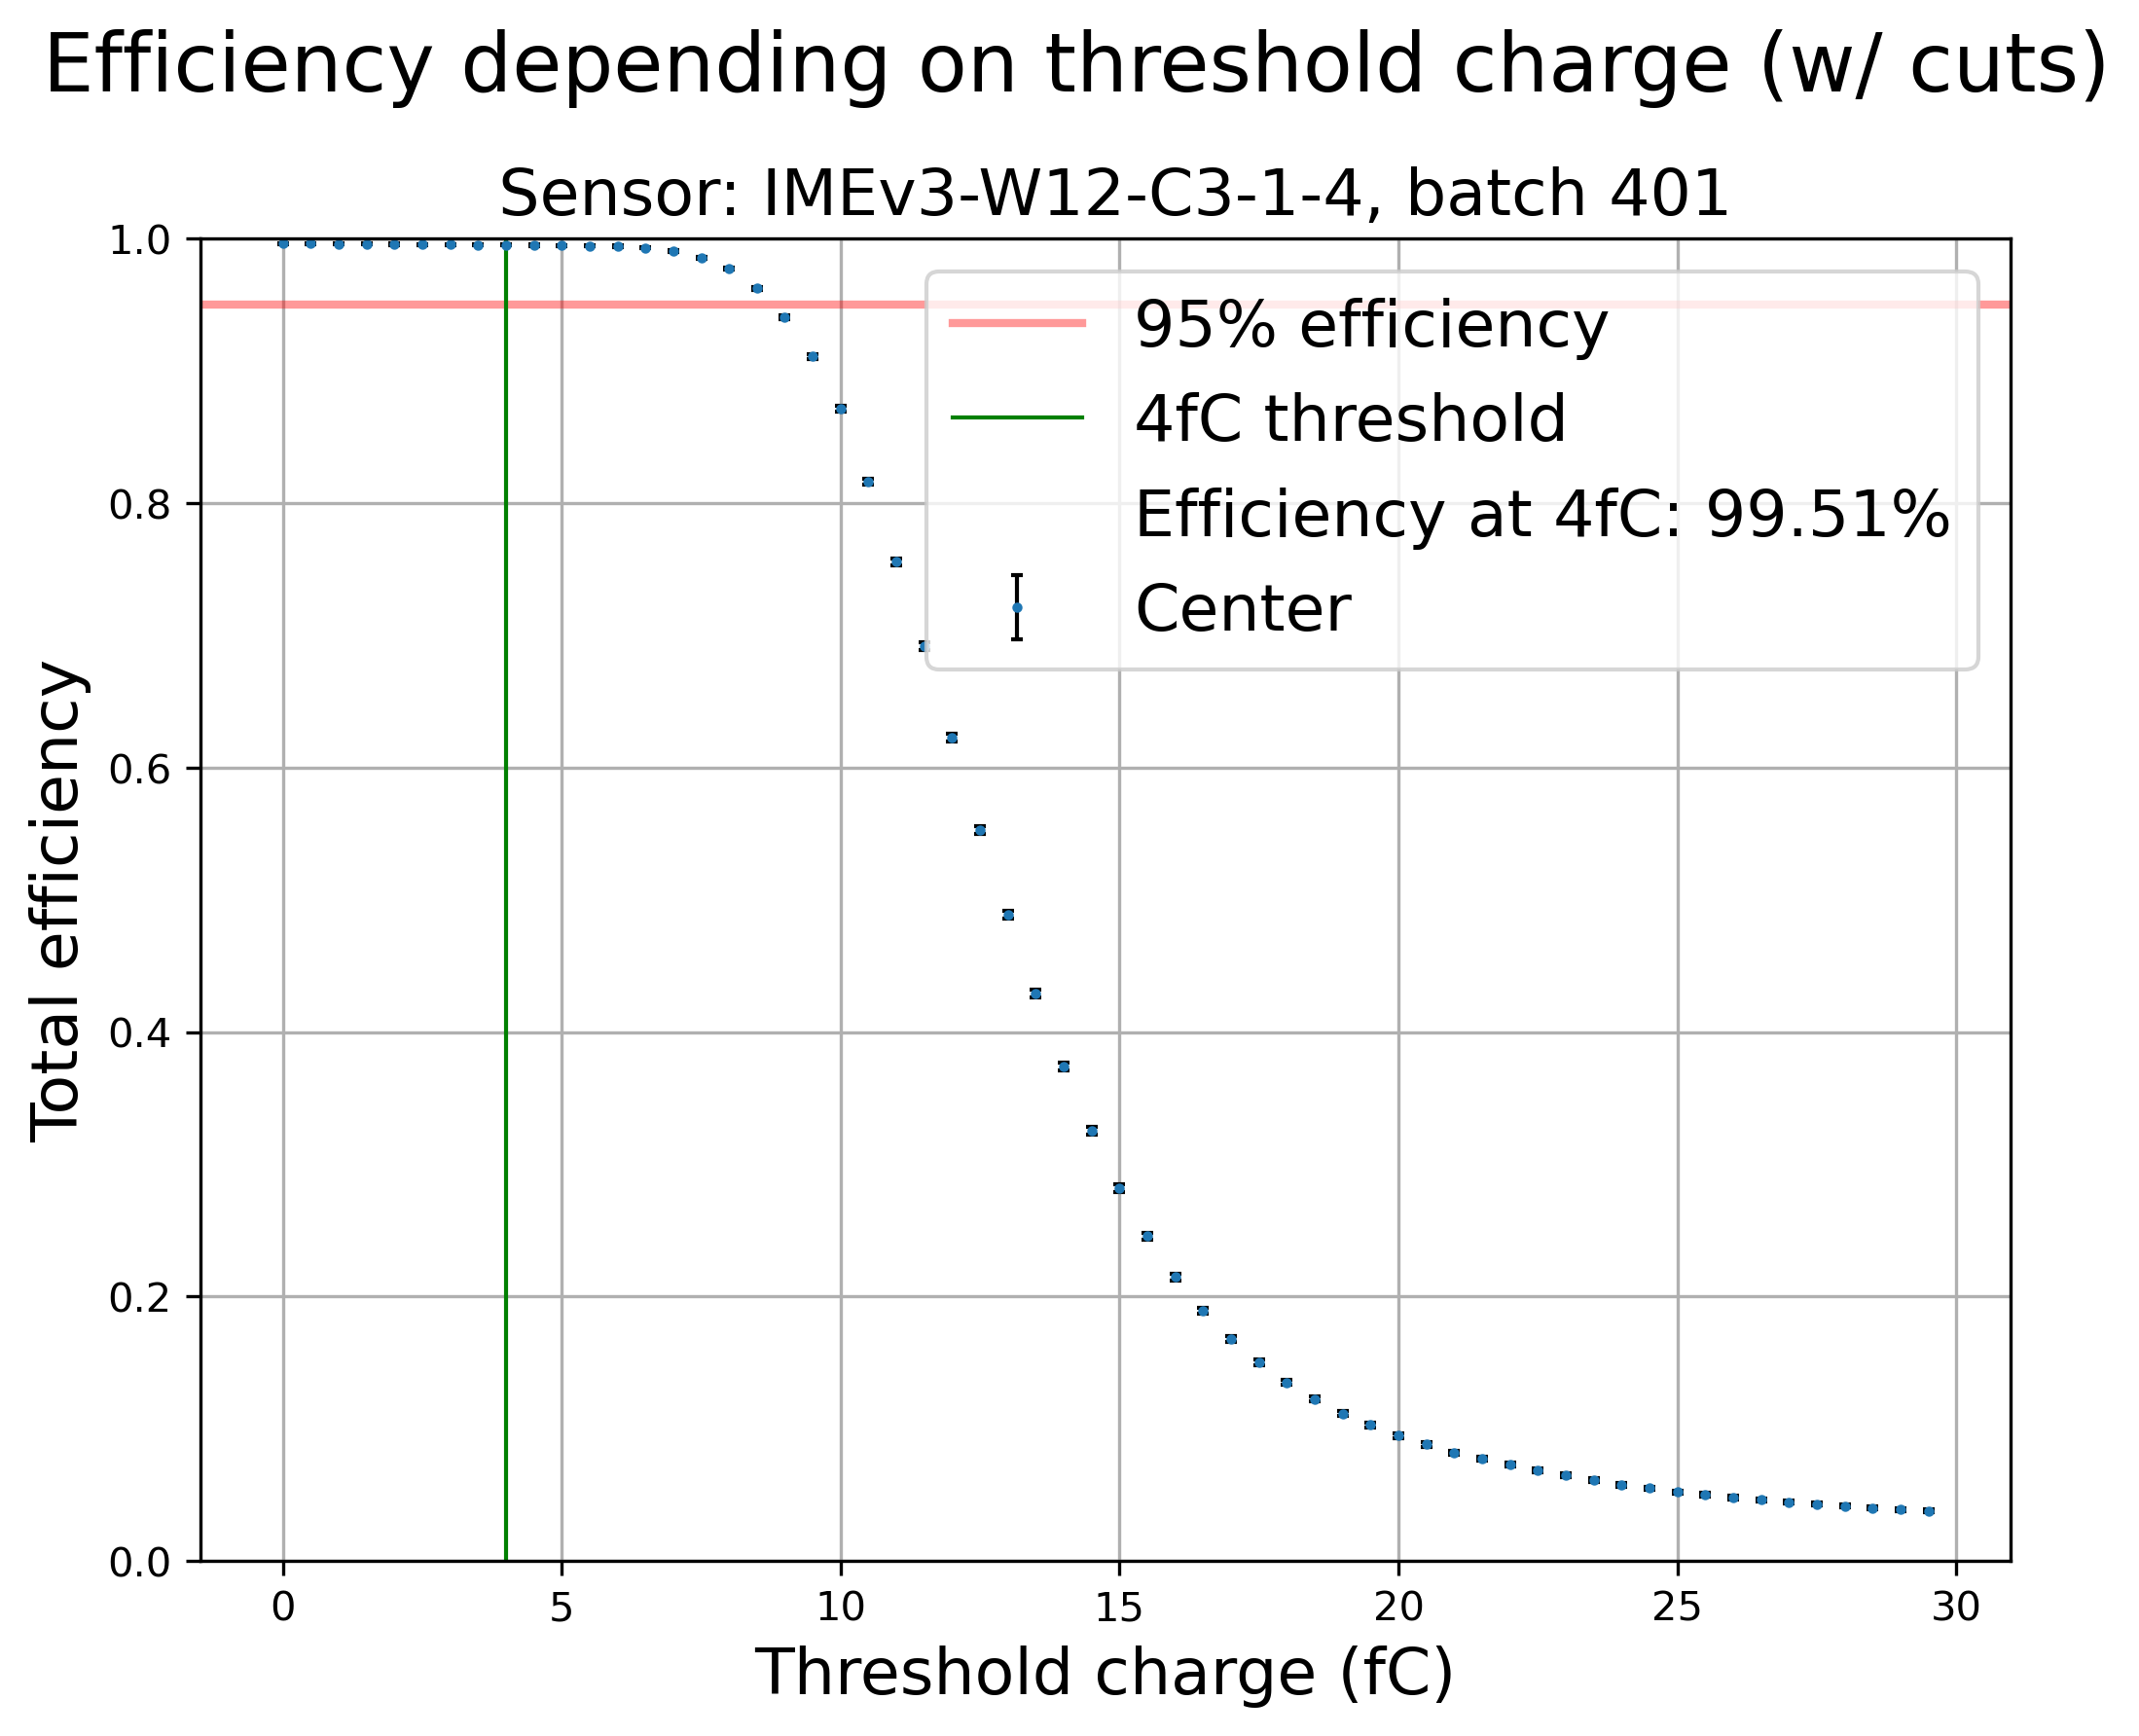
\includegraphics[width=0.5\linewidth]{Images/efficiency_plots/Efficiency depending on threshold charge (with cuts) batch 401 S1.png}
    \caption{Total efficiency when changing the threshold value, ensuring that there is a large plateau of high efficiency.}
    \label{fig:efficiency_depending_threshold}
\end{figure}


\section{Time Resolution}\label{sec:methods_time_resolution}

The difference of times of arrival between the DUT and the MCP was fitted with a normal distribution. The standard deviation of said distribution corresponded to the time resolution of the DUT and MCP combined. Using simple error propagation, the time resolution of the DUT was computed: 

\begin{equation*}
    \begin{gathered}
    \sigma_{dut+MCP} = \sigma_{dut} \oplus \sigma_{MCP} \\
    \downarrow \\
    \sigma_{dut+MCP}^2 = \sigma_{dut}^2 + \sigma_{MCP}^2 \\
    \sigma_{dut} = \sqrt{\sigma_{dut+MCP}^2-\sigma_{MCP}^2}  \, .
    \end{gathered}
\end{equation*}

For this sensor (Figure~\ref{fig:time_resolution_plot}) the final time resolution was \(\sigma_{dut} = 49.38\pm0.81\si{\ps} \)

\begin{figure}[h!tbp]
    \centering
    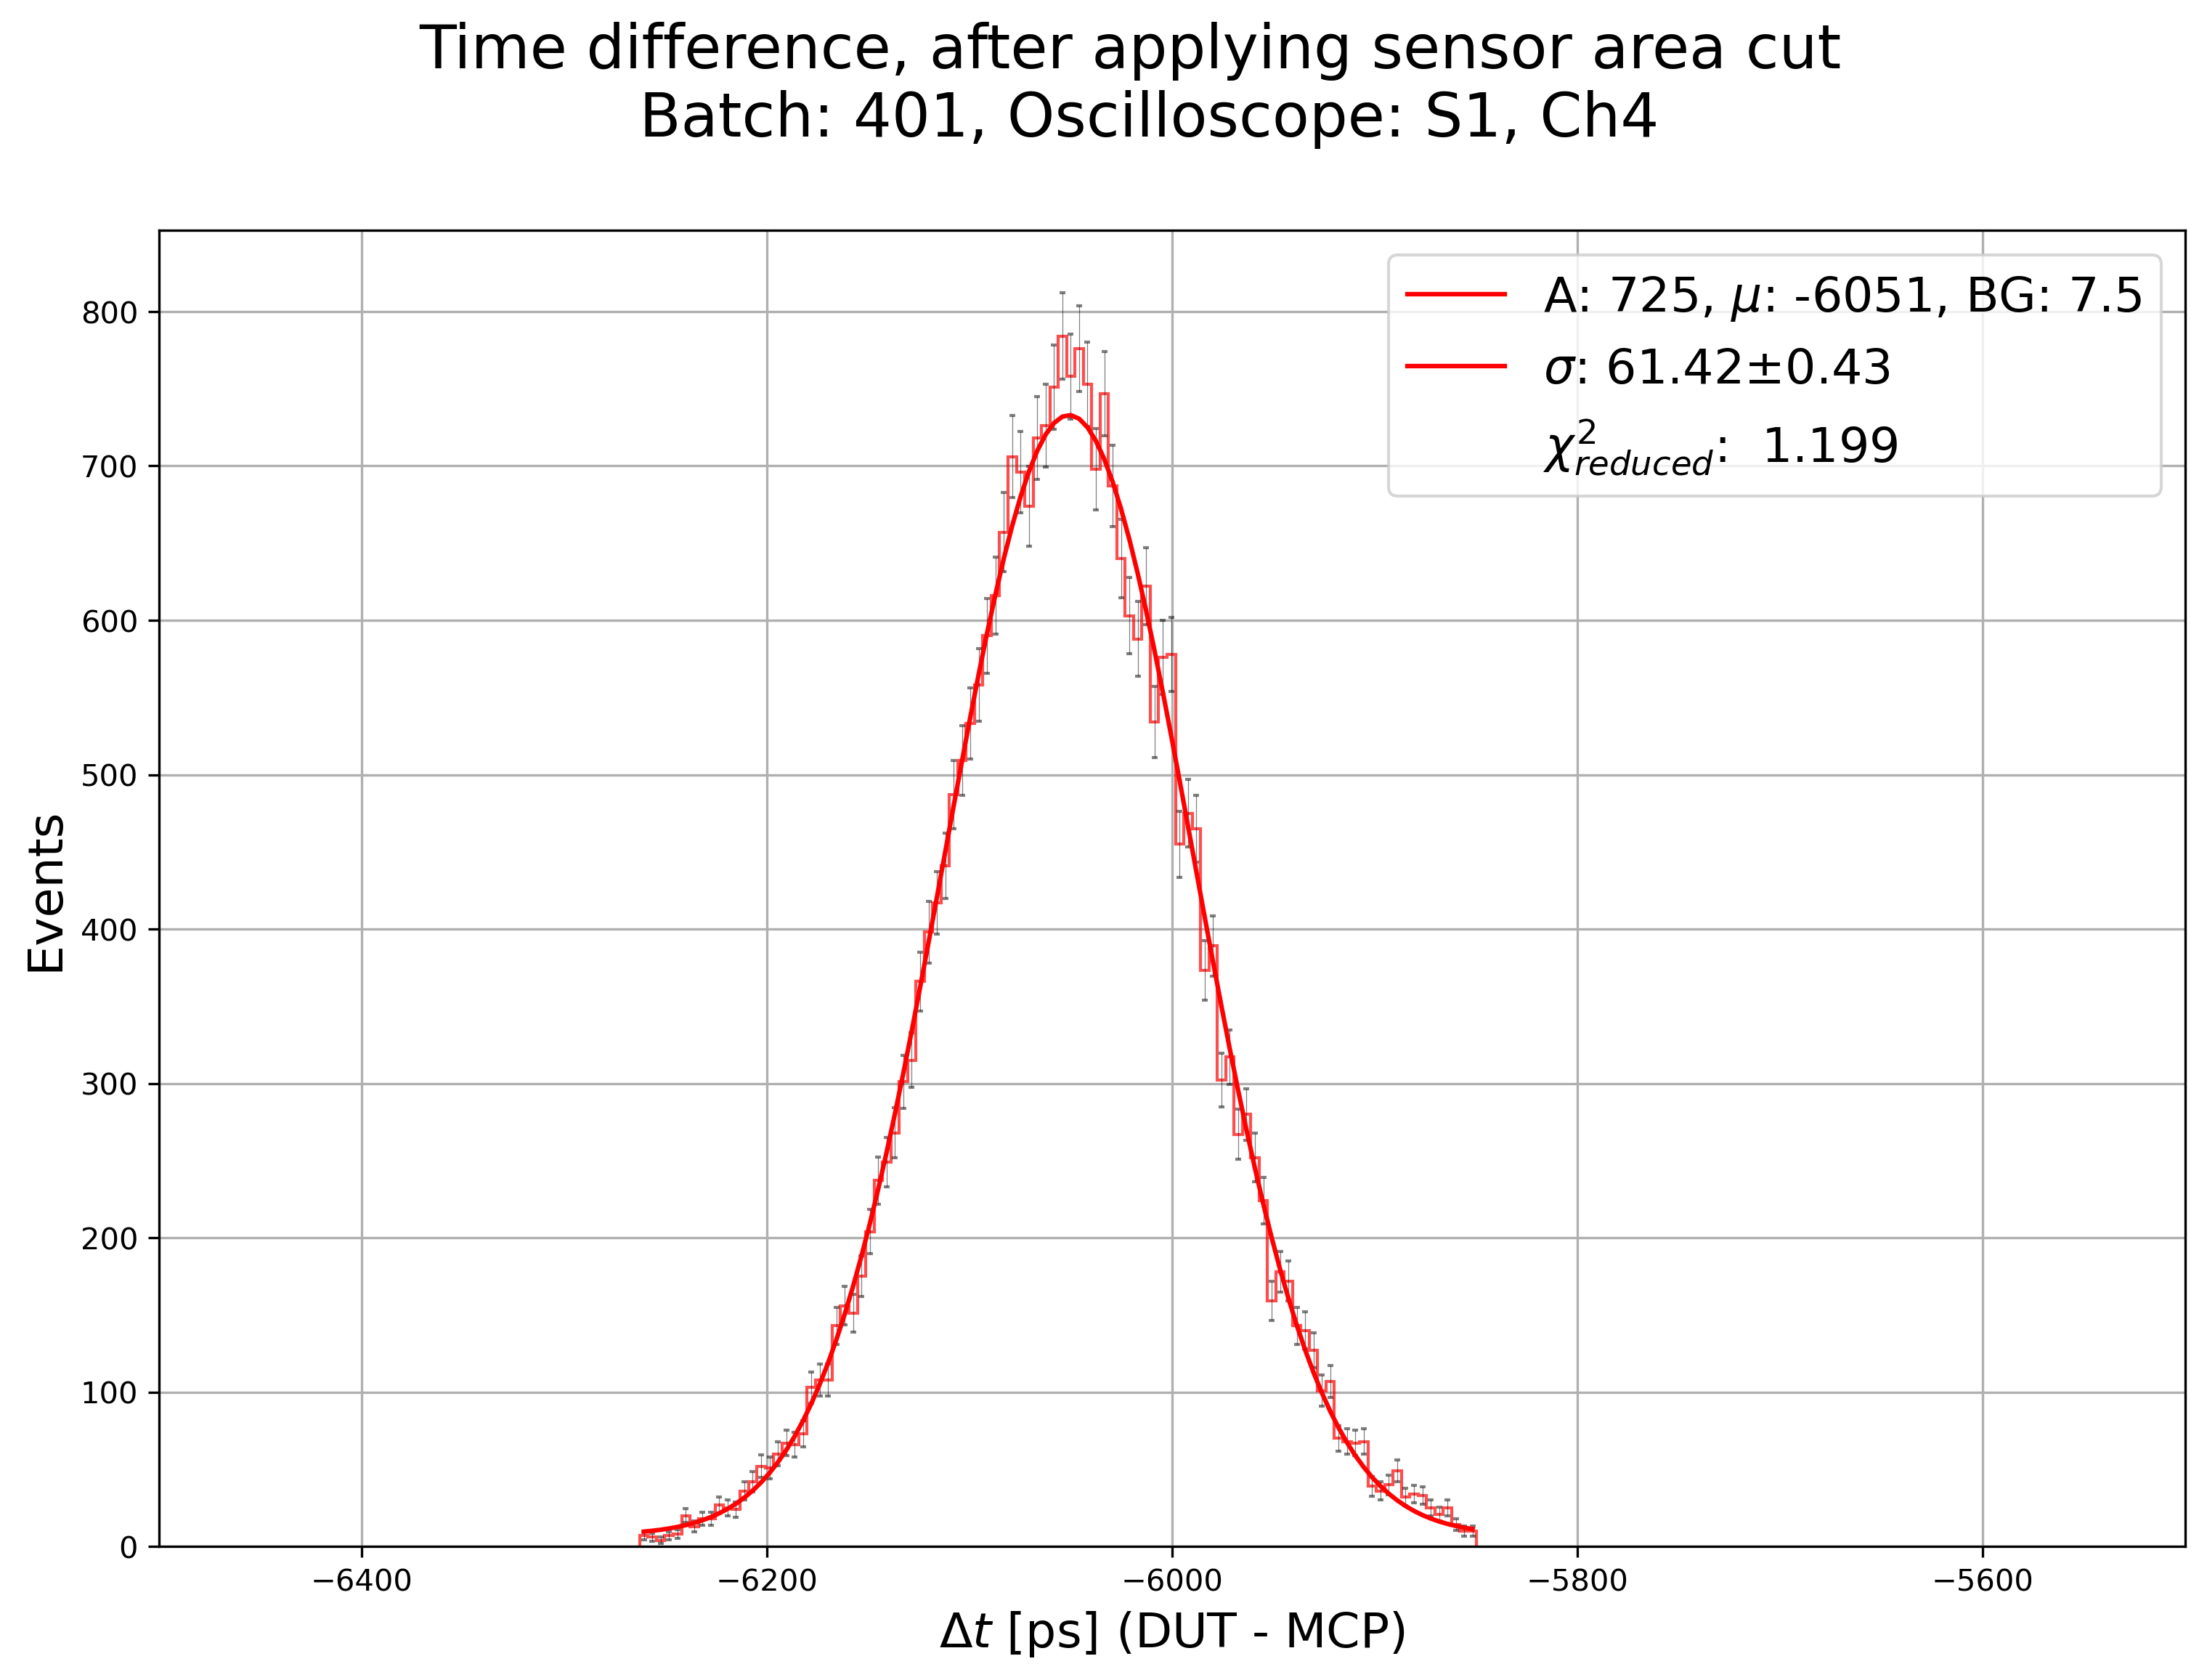
\includegraphics[width=0.7\linewidth]{Images/time_resolution_plots/time_difference_401_S1_zoomed_and_gauss_fit_with_cuts_central_area_DUTs_3.png}
    \captionsetup{width=\captionwidth}
    \caption{Gaussian fit of \(\Delta t\) to find the time resolution (\(\sigma\)), the error bars are the statistical poissonian error (\(y_{err}=\sqrt{N}\)).}
    \label{fig:time_resolution_plot}
\end{figure}




\chapter{Results}
\marginpar{file to be created}

\chapter{Conclusions}
\marginpar{file to make}

\appendix

%%% APPENDIX
\chapter{Appendix}\label{chap:appendix}

Additional explanations:
\marginpar{\flushleft make into actual Appendix type}
\section{Complete list of DUTs}

\begin{landscape}

\begin{table}[h]
    \caption{Complete list of the tested devices with additional details}
    \label{tab:full_devices_tested}
    \footnotesize
        \begin{tabularx}{\textheight}{|l|l|l|l|l|l|l|l|X|}
            \hline
            \textbf{Device name} & \textbf{Vendor} & \textbf{Sensor ID} &  \begin{tabular}{@{}l@{}}\textbf{Pads,} \\ \textbf{used channels}\end{tabular} & \begin{tabular}{@{}l@{}}\textbf{Fluence} \\ $[n_{eq}/\si{cm^2}]$ \end{tabular} &\begin{tabular}{@{}l@{}} \textbf{Radiation} \\ \textbf{type} \end{tabular} & \textbf{Board name} & \begin{tabular}{@{}l@{}}\textbf{Board} \\ \textbf{channels} \end{tabular} & \textbf{Notes} \\
            \hline
            CNM-W4 & CNM & CNM-R15973-W4-D168 & single & 0 & - & JSI-B12 & - & reference \\ 
            CNM-W5 & CNM & CNM-R15973-W5-D138 & single & 0 & - & JSI-B14 & - & reference \\ 
            CNM-W5-1.5E15 & CNM & CNM-R15973-W5-D29 & single & $\num{1.50E+15}$ & neutron & JSI-B5 & - & \\ 
            CNM-W3-2.5E15 & CNM & CNM-R15973-W3-D29 & single & $\num{2.50E+15}$ & neutron & JSI-PP1 & - & \\
            USTC2.1-W17 & USTC & USTC2.1-W17-P6-A-2x2 & 2x2, 2 channels & 0 & - & CERN-3 & Ch1,Ch2 & \\
            USTC2.1-W19 & USTC & USTC2.1-W19-P5-A-1x1 & single & 0 & - & CERN-3 & - & not tested \\
            USTC2.1-W17-2E14 & USTC & USTC2.1-W17-P6-A-2x2 & 2x2, 1 channel & 0 & - & JSI-B2 & - & missing \\ 
            IMEv3-W12-2x2 & IHEP & IMEv3-W12-C2-2-2 & 2x2, 2 channels & 0 & - & CERN-1 & Ch1,Ch2 &  \\ 
            IMEv3-W12-1x3 & IHEP & IMEv3-W12-C3-1-4(and5) & 1x3, 2 channels & 0 & - & CERN-1 & Ch3,Ch4 &  \\ 
            IMEv3-W12-2x2-1.5E15 & IHEP & IMEv3-W12-B2-2-9-1 & 2x2, 3 channels & $\num{1.50E+15}$ & neutron & CERN-2 & Ch0,Ch1,Ch2 &  \\ 
            IMEv3-W16-1x3-1.5E15 & IHEP & IMEv3-W16-Q4-D4-1-4 & 1x3, 1 channel & $\num{1.50E+15}$ & neutron & CERN-2 & Ch3 &  \\ 
            IMEv2-W7-1E14 & IHEP & W7-II-C2-1-7IMEv2-W7Q2 & single & $\num{1.00E+14}$ & proton & JSI-B6 & - &  \\ 
            IMEv2-W7-6.5E14 & IHEP & W7-II-C2-1-7IMEv2-W7Q2 & single & $\num{6.50E+14}$ & proton & JSI-PP4 & - &  \\ 
            IMEv3-W16-8E14 & IHEP & IHEP-IMEv3-W16-Q4-D3-1-4 & single & $\num{8.00E+14}$ & proton & JSI-B7 & - &  \\ 
            IMEv3-W16-2.5E15 & IHEP & IHEP-IMEv3-W16-Q4-E3-1-4 & single & $\num{2.50E+15}$ & neutron & JSI-B13 & - &  \\ 
            \hline
        \end{tabularx}
\end{table}
\end{landscape}


\section{Empty vertical line}
Due to one dead column of pixels of a MIMOSA \marginpar{\flushleft add plots of the DATA showing the vertical line, or link/ref to it} some batches presented an empty vertical line. The cause of this was found in one of the MIMOSA planes, which had a dead column of pixels and interfered with the track reconstruction. This problem turned out to be inconsequential for the analysis, except for the very low statistics in that very small region.
\begin{figure}[!ht]
    \centering
    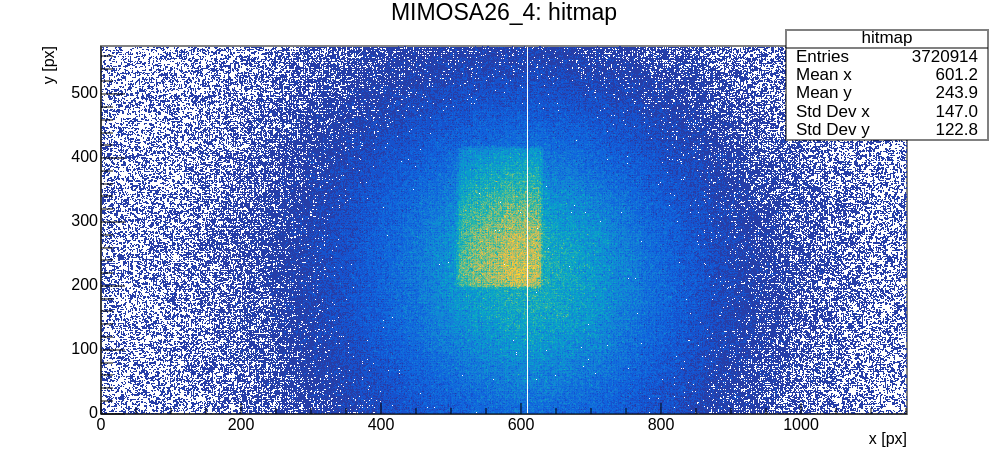
\includegraphics[width=.9\linewidth]{Images/appendix/hits_MIMOSA4.png}
    \caption{The hits heatmap of the MIMOSA plane n°4, which shows clearly the source of the "empty line" that appeared in the data.}
    \label{fig:MIMOSA4_hits}
\end{figure}


\section[Vavilov vs Landau distribution]{On the Vavilov distribution approximation}\label{sec:vavilov_vs_landau_distribution}

% \cite[189]{NAP20066}
%     
% \maketitle
    
\begin{tcolorbox}[breakable, size=fbox, boxrule=1pt, pad at break*=1mm,colback=cellbackground, colframe=cellborder]
\prompt{In}{incolor}{1}{\boxspacing}
\begin{Verbatim}[commandchars=\\\{\}]
\PY{k+kn}{import} \PY{n+nn}{numpy} \PY{k}{as} \PY{n+nn}{np} \PY{c+c1}{\PYZsh{} NumPy}
\PY{k+kn}{from} \PY{n+nn}{scipy}\PY{n+nn}{.}\PY{n+nn}{optimize} \PY{k+kn}{import} \PY{n}{fsolve} 
\PY{k+kn}{from} \PY{n+nn}{IPython}\PY{n+nn}{.}\PY{n+nn}{display} \PY{k+kn}{import} \PY{n}{Image}
\PY{k+kn}{import} \PY{n+nn}{pandas} \PY{k}{as} \PY{n+nn}{pd} \PY{c+c1}{\PYZsh{} Pandas}
\PY{n}{pd}\PY{o}{.}\PY{n}{options}\PY{o}{.}\PY{n}{display}\PY{o}{.}\PY{n}{float\PYZus{}format} \PY{o}{=} \PY{l+s+s1}{\PYZsq{}}\PY{l+s+si}{\PYZob{}:5,.4E\PYZcb{}}\PY{l+s+s1}{\PYZsq{}}\PY{o}{.}\PY{n}{format}
\end{Verbatim}
\end{tcolorbox}

    \hypertarget{calculating-the-factor-the-determines-if-the-vavilov-distribution-can-be-approximated-by-a-landau}{%
\section{Calculating the factor the determines if the Vavilov
distribution can be approximated by a
Landau}\label{calculating-the-factor-the-determines-if-the-vavilov-distribution-can-be-approximated-by-a-landau}}

Bethe-Bloch mean energy loss: \[
\left\langle-\frac{dE}{dx} \right\rangle \frac{1}{\rho} =  K z_0^2 \frac{1}{\beta^2} \frac{Z}{A M_u} \cdot\left[\frac{1}{2}\ln \left(\frac{2m_e c^2 \beta^2 W_{max}}{I^2 \cdot (1-\beta^2)}\right) - \beta^2\right]
\]

\[
K/M_u = 4 \pi N_A r_e^2 m_e c^2 /M_u = 0.307075\space \text{MeV g}^{-1} \text{cm}^2
\]

\[
r_e  = \frac{e^2}{4\pi\varepsilon_0 m_e c^2} \\
M_u = 1 \frac{g}{mol} \quad z_0=1 \\
\left( W_{max} \equiv \epsilon_{max} \right)
\]

For \textbf{silicon}: \[
Z = 14 \\
A = 28.085 \\ 
\rho = 2.329085 \text{  g cm}^{-3}\\
I = 173 \text{ eV} % \quad \text{(mean excitation energy)}
\]

\hypertarget{calculating-beta-for-a-proton-of-energy-e_k}{%
\subsubsection{\texorpdfstring{Calculating \(\beta\) for a proton of
energy
\(E_k\)}{Calculating \textbackslash beta for a proton of energy E\_k}}\label{calculating-beta-for-a-proton-of-energy-e_k}}

\[
E_k = (\gamma - 1) m_o c^2 \\
\gamma = \frac{E_k + m_o c^2}{m_o c^2} \\
\beta^2 = 1 - \left(\frac{m_o c^2}{E_k +m_o c^2} \right)^2
\]

for a proton of energy \(E_k=120\space \text{GeV}\),
\(m_0 = 938.272\space \text{MeV/c}^2\)

    \begin{tcolorbox}[breakable, size=fbox, boxrule=1pt, pad at break*=1mm,colback=cellbackground, colframe=cellborder]
\prompt{In}{incolor}{2}{\boxspacing}
\begin{Verbatim}[commandchars=\\\{\}]
\PY{n}{energy} \PY{o}{=} \PY{l+m+mf}{120e3} \PY{c+c1}{\PYZsh{} MeV  (120 GeV)}
\PY{c+c1}{\PYZsh{} m\PYZus{}particle = 938.272088 \PYZsh{} MeV/c\PYZca{}2  protons }
\PY{n}{m\PYZus{}particle} \PY{o}{=} \PY{l+m+mf}{938.213} \PY{c+c1}{\PYZsh{} MeV/c\PYZca{}2     protons (older value)}

\PY{n}{gamma} \PY{o}{=} \PY{p}{(}\PY{n}{energy} \PY{o}{+} \PY{n}{m\PYZus{}particle}\PY{p}{)}\PY{o}{/}\PY{n}{m\PYZus{}particle}
\PY{n}{beta\PYZus{}2} \PY{o}{=} \PY{l+m+mi}{1} \PY{o}{\PYZhy{}} \PY{n}{m\PYZus{}particle}\PY{o}{*}\PY{o}{*}\PY{l+m+mi}{2}\PY{o}{/}\PY{p}{(}\PY{n}{m\PYZus{}particle} \PY{o}{+} \PY{n}{energy}\PY{p}{)}\PY{o}{*}\PY{o}{*}\PY{l+m+mi}{2}

\PY{n+nb}{print}\PY{p}{(}\PY{l+s+s2}{\PYZdq{}}\PY{l+s+s2}{ gamma: }\PY{l+s+s2}{\PYZdq{}}\PY{p}{,} \PY{n}{gamma}\PY{p}{,} \PY{l+s+s2}{\PYZdq{}}\PY{l+s+se}{\PYZbs{}n}\PY{l+s+s2}{\PYZdq{}}\PY{p}{,} \PY{l+s+s2}{\PYZdq{}}\PY{l+s+s2}{beta²: }\PY{l+s+s2}{\PYZdq{}}\PY{p}{,} \PY{n}{beta\PYZus{}2}\PY{p}{)}
\end{Verbatim}
\end{tcolorbox}

    \begin{Verbatim}[commandchars=\\\{\}]
 gamma:  128.90272571367058
 beta²:  0.999939816727599
    \end{Verbatim}

    from https://academic.oup.com/book/43645/chapter/365027598\#404941541 :

The parameter \(\kappa\) of the Vavilov distribution determines if it
becomes close to a Landau (\(\kappa\rightarrow0\)) or a Gaussian
(\(\kappa 10\)).

To calculate \(\kappa\): 
\[
\kappa = \frac{\xi}{\epsilon_{max}}
\]

where: \[
\xi = \frac{1}{2} K \frac{Z}{A} \frac{s} {\beta^2}
\]

\(s = \Delta x \cdot \rho\)

and from https://nap.nationalacademies.org/read/20066/chapter/10\#188 :
\[
\epsilon_{max} = \frac{2m_e c^2 \beta^2}{1-\beta^2}\left[ 1 + \frac{2m_e}{M}\frac{1}{\sqrt{1-\beta^2}} + \left(\frac{m_e}{M}\right)^2 \right]^{-1}
\]

where \(M\) is the mass of the incoming particle.

Also written as:

\[
\epsilon_{max} = \frac{2m_e c^2 \beta^2 \gamma^2} { 1 + \frac{2\gamma m_e}{M} + \left(\frac{m_e}{M}\right)^2}
\]

    \hypertarget{applying-this-to-a-thin-silicon-layer-50mu-textm}{%
\subsubsection{\texorpdfstring{Applying this to a thin silicon layer
(50\(\mu \text{m}\))}{Applying this to a thin silicon layer (50\textbackslash mu \textbackslash text\{m\})}}\label{applying-this-to-a-thin-silicon-layer-50mu-textm}}

(The masses are either multiplied by \(c^2\) or in a ratio, the mass
units used are \(\text{MeV}/c^2\))

    \begin{tcolorbox}[breakable, size=fbox, boxrule=1pt, pad at break*=1mm,colback=cellbackground, colframe=cellborder]
\prompt{In}{incolor}{3}{\boxspacing}
\begin{Verbatim}[commandchars=\\\{\}]
\PY{c+c1}{\PYZsh{}\PYZsh{}\PYZsh{} variables values}
\PY{n}{m\PYZus{}electron} \PY{o}{=} \PY{l+m+mf}{0.51099895} \PY{c+c1}{\PYZsh{} MeV/c\PYZca{}2}
\PY{n}{z\PYZus{}0} \PY{o}{=} \PY{l+m+mi}{1} \PY{c+c1}{\PYZsh{} electric charge of incoming particle}
\PY{n}{delta\PYZus{}x} \PY{o}{=} \PY{l+m+mf}{5e\PYZhy{}3} \PY{c+c1}{\PYZsh{} cm  (50um)}

\PY{c+c1}{\PYZsh{}\PYZsh{}\PYZsh{} silicon}
\PY{n}{Z} \PY{o}{=} \PY{l+m+mi}{14}   \PY{c+c1}{\PYZsh{} atomic number}
\PY{n}{A} \PY{o}{=} \PY{l+m+mf}{28.085}  \PY{c+c1}{\PYZsh{} atomic weight}
\PY{n}{density} \PY{o}{=} \PY{l+m+mf}{2.329085} \PY{c+c1}{\PYZsh{} g cm\PYZca{}\PYZhy{}3}
\PY{n}{mean\PYZus{}excitation} \PY{o}{=} \PY{l+m+mf}{173e\PYZhy{}6} \PY{c+c1}{\PYZsh{} MeV  (mean excitation energy of Silicon: 173 eV)}

\PY{n}{s} \PY{o}{=} \PY{n}{delta\PYZus{}x} \PY{o}{*} \PY{n}{density} \PY{c+c1}{\PYZsh{} g cm\PYZca{}\PYZhy{}2}
\PY{n}{K} \PY{o}{=} \PY{l+m+mf}{0.307075} \PY{c+c1}{\PYZsh{} MeV g\PYZca{}\PYZhy{}1 cm\PYZca{}2}
\end{Verbatim}
\end{tcolorbox}

    \begin{tcolorbox}[breakable, size=fbox, boxrule=1pt, pad at break*=1mm,colback=cellbackground, colframe=cellborder]
\prompt{In}{incolor}{4}{\boxspacing}
\begin{Verbatim}[commandchars=\\\{\}]
\PY{k}{def} \PY{n+nf}{xi\PYZus{}func}\PY{p}{(}\PY{n}{energy}\PY{p}{)}\PY{p}{:}
    \PY{n}{beta\PYZus{}2} \PY{o}{=} \PY{l+m+mi}{1} \PY{o}{\PYZhy{}} \PY{n}{m\PYZus{}particle}\PY{o}{*}\PY{o}{*}\PY{l+m+mi}{2}\PY{o}{/}\PY{p}{(}\PY{n}{m\PYZus{}particle} \PY{o}{+} \PY{n}{energy}\PY{p}{)}\PY{o}{*}\PY{o}{*}\PY{l+m+mi}{2}
    \PY{k}{return} \PY{p}{(}\PY{l+m+mi}{1}\PY{o}{/}\PY{l+m+mi}{2} \PY{o}{*} \PY{n}{K}\PY{p}{)} \PY{o}{*} \PY{p}{(}\PY{n}{Z} \PY{o}{/} \PY{n}{A}\PY{p}{)} \PY{o}{*} \PY{p}{(}\PY{n}{s} \PY{o}{/} \PY{n}{beta\PYZus{}2}\PY{p}{)}

\PY{k}{def} \PY{n+nf}{eps\PYZus{}max\PYZus{}func}\PY{p}{(}\PY{n}{energy}\PY{p}{)}\PY{p}{:}
    \PY{n}{gamma} \PY{o}{=} \PY{p}{(}\PY{n}{energy} \PY{o}{+} \PY{n}{m\PYZus{}particle}\PY{p}{)}\PY{o}{/}\PY{n}{m\PYZus{}particle}
    \PY{n}{beta\PYZus{}2} \PY{o}{=} \PY{l+m+mi}{1} \PY{o}{\PYZhy{}} \PY{n}{m\PYZus{}particle}\PY{o}{*}\PY{o}{*}\PY{l+m+mi}{2}\PY{o}{/}\PY{p}{(}\PY{n}{m\PYZus{}particle} \PY{o}{+} \PY{n}{energy}\PY{p}{)}\PY{o}{*}\PY{o}{*}\PY{l+m+mi}{2}
    \PY{k}{return} \PY{p}{(}\PY{l+m+mi}{2} \PY{o}{*} \PY{n}{m\PYZus{}electron} \PY{o}{*} \PY{n}{beta\PYZus{}2} \PY{o}{*} \PY{n}{gamma}\PY{o}{*}\PY{o}{*}\PY{l+m+mi}{2}\PY{p}{)} \PY{o}{/} \PY{p}{(}\PY{l+m+mi}{1} \PY{o}{+} \PY{l+m+mi}{2}\PY{o}{*}\PY{n}{gamma}\PY{o}{*}\PY{n}{m\PYZus{}electron}\PY{o}{/}\PY{n}{m\PYZus{}particle} \PY{o}{+} \PY{p}{(}\PY{n}{m\PYZus{}electron}\PY{o}{/}\PY{n}{m\PYZus{}particle}\PY{p}{)}\PY{o}{*}\PY{o}{*}\PY{l+m+mi}{2}\PY{p}{)} \PY{c+c1}{\PYZsh{} MeV}

\PY{k}{def} \PY{n+nf}{kappa\PYZus{}func}\PY{p}{(}\PY{n}{energy}\PY{p}{,} \PY{n}{kappa\PYZus{}value}\PY{o}{=}\PY{l+m+mf}{0.01}\PY{p}{)}\PY{p}{:}
    \PY{l+s+sd}{\PYZdq{}\PYZdq{}\PYZdq{}kappa as a function of the energy (to find the zeros for k=kappa\PYZus{}value)\PYZdq{}\PYZdq{}\PYZdq{}}
    \PY{n}{gamma} \PY{o}{=} \PY{p}{(}\PY{n}{energy} \PY{o}{+} \PY{n}{m\PYZus{}particle}\PY{p}{)}\PY{o}{/}\PY{n}{m\PYZus{}particle}
    \PY{n}{beta\PYZus{}2} \PY{o}{=} \PY{l+m+mi}{1} \PY{o}{\PYZhy{}} \PY{n}{m\PYZus{}particle}\PY{o}{*}\PY{o}{*}\PY{l+m+mi}{2}\PY{o}{/}\PY{p}{(}\PY{n}{m\PYZus{}particle} \PY{o}{+} \PY{n}{energy}\PY{p}{)}\PY{o}{*}\PY{o}{*}\PY{l+m+mi}{2}
    \PY{k}{return} \PY{n}{xi\PYZus{}func}\PY{p}{(}\PY{n}{energy}\PY{p}{)} \PY{o}{/} \PY{n}{eps\PYZus{}max\PYZus{}func}\PY{p}{(}\PY{n}{energy}\PY{p}{)} \PY{o}{\PYZhy{}} \PY{n}{kappa\PYZus{}value}
\end{Verbatim}
\end{tcolorbox}

    \begin{tcolorbox}[breakable, size=fbox, boxrule=1pt, pad at break*=1mm,colback=cellbackground, colframe=cellborder]
\prompt{In}{incolor}{5}{\boxspacing}
\begin{Verbatim}[commandchars=\\\{\}]
\PY{n}{xi} \PY{o}{=} \PY{p}{(}\PY{l+m+mi}{1}\PY{o}{/}\PY{l+m+mi}{2} \PY{o}{*} \PY{n}{K}\PY{p}{)} \PY{o}{*} \PY{p}{(}\PY{n}{Z} \PY{o}{/} \PY{n}{A}\PY{p}{)} \PY{o}{*} \PY{p}{(}\PY{n}{s} \PY{o}{/} \PY{n}{beta\PYZus{}2}\PY{p}{)} \PY{c+c1}{\PYZsh{} MeV}

\PY{n}{epsilon\PYZus{}max} \PY{o}{=} \PY{n}{eps\PYZus{}max\PYZus{}func}\PY{p}{(}\PY{n}{energy}\PY{p}{)} \PY{c+c1}{\PYZsh{} MeV}

\PY{n}{kappa} \PY{o}{=} \PY{n}{xi} \PY{o}{/} \PY{n}{epsilon\PYZus{}max}

\PY{n+nb}{print}\PY{p}{(}\PY{l+s+s2}{\PYZdq{}}\PY{l+s+s2}{k =}\PY{l+s+s2}{\PYZdq{}}\PY{p}{,}\PY{n}{kappa}\PY{p}{)}
\end{Verbatim}
\end{tcolorbox}

    \begin{Verbatim}[commandchars=\\\{\}]
k = 5.98637846070628e-08
    \end{Verbatim}

    \hypertarget{comparison-with-calculations-from-httpsnap.nationalacademies.orgread20066chapter10189}{%
\subsection{Comparison with calculations from \cite{NAP20066} }\label{comparison-with-calculations-from-httpsnap.nationalacademies.orgread20066chapter10189}}

    \begin{tcolorbox}[breakable, size=fbox, boxrule=1pt, pad at break*=1mm,colback=cellbackground, colframe=cellborder]
\prompt{In}{incolor}{6}{\boxspacing}
\begin{Verbatim}[commandchars=\\\{\}]
\PY{n}{Image}\PY{p}{(}\PY{l+s+s2}{\PYZdq{}}\PY{l+s+s2}{epsilon and xi formulas.png}\PY{l+s+s2}{\PYZdq{}}\PY{p}{,} \PY{n}{width}\PY{o}{=}\PY{l+m+mi}{1000}\PY{p}{)}
\end{Verbatim}
\end{tcolorbox}
 
            
\prompt{Out}{outcolor}{6}{}
    
    \begin{center}
    \adjustimage{max size={0.9\linewidth}{0.9\paperheight}}{Chapters/Vavilov_Landau/output_10_0.png}
    \end{center}
    { \hspace*{\fill} \\}
    

    Then follows a table with the values calculated for different energies:

    \begin{tcolorbox}[breakable, size=fbox, boxrule=1pt, pad at break*=1mm,colback=cellbackground, colframe=cellborder]
\prompt{In}{incolor}{7}{\boxspacing}
\begin{Verbatim}[commandchars=\\\{\}]
\PY{n}{Image}\PY{p}{(}\PY{l+s+s2}{\PYZdq{}}\PY{l+s+s2}{Table of k and xi values.png}\PY{l+s+s2}{\PYZdq{}}\PY{p}{,} \PY{n}{width}\PY{o}{=}\PY{l+m+mi}{800}\PY{p}{)}
\end{Verbatim}
\end{tcolorbox}
 
            
\prompt{Out}{outcolor}{7}{}
    
    \begin{center}
    \adjustimage{max size={0.9\linewidth}{0.9\paperheight}}{Chapters/Vavilov_Landau/output_12_0.png}
    \end{center}
    { \hspace*{\fill} \\}
    

    Comparison of these values with my previous calculations

    \begin{tcolorbox}[breakable, size=fbox, boxrule=1pt, pad at break*=1mm,colback=cellbackground, colframe=cellborder]
\prompt{In}{incolor}{8}{\boxspacing}
\begin{Verbatim}[commandchars=\\\{\}]
\PY{c+c1}{\PYZsh{} Values from 100 MeV to 10 GeV}
\PY{n}{energy\PYZus{}array} \PY{o}{=} \PY{n}{np}\PY{o}{.}\PY{n}{array}\PY{p}{(}\PY{p}{[}\PY{l+m+mi}{100}\PY{p}{,}\PY{l+m+mi}{150}\PY{p}{,}\PY{l+m+mi}{200}\PY{p}{,}\PY{l+m+mi}{300}\PY{p}{,}\PY{l+m+mi}{400}\PY{p}{,}\PY{l+m+mi}{500}\PY{p}{,}\PY{l+m+mi}{600}\PY{p}{,}\PY{l+m+mi}{800}\PY{p}{,}\PY{l+m+mi}{1000}\PY{p}{,}\PY{l+m+mi}{1500}\PY{p}{,}\PY{l+m+mi}{2000}\PY{p}{,}\PY{l+m+mi}{3000}\PY{p}{,}\PY{l+m+mi}{4000}\PY{p}{,}\PY{l+m+mi}{5000}\PY{p}{,}\PY{l+m+mi}{6000}\PY{p}{,}\PY{l+m+mi}{8000}\PY{p}{,}\PY{l+m+mi}{10000}\PY{p}{]}\PY{p}{)}
\end{Verbatim}
\end{tcolorbox}

    \begin{tcolorbox}[breakable, size=fbox, boxrule=1pt, pad at break*=1mm,colback=cellbackground, colframe=cellborder]
\prompt{In}{incolor}{9}{\boxspacing}
\begin{Verbatim}[commandchars=\\\{\}]
\PY{n}{table\PYZus{}data} \PY{o}{=} \PY{n}{np}\PY{o}{.}\PY{n}{vstack}\PY{p}{(}\PY{p}{(}\PY{l+m+mi}{1} \PY{o}{\PYZhy{}} \PY{n}{m\PYZus{}particle}\PY{o}{*}\PY{o}{*}\PY{l+m+mi}{2} \PY{o}{/} \PY{p}{(}\PY{n}{m\PYZus{}particle}\PY{o}{+}\PY{n}{energy\PYZus{}array}\PY{p}{)}\PY{o}{*}\PY{o}{*}\PY{l+m+mi}{2}\PY{p}{,}
              \PY{n}{eps\PYZus{}max\PYZus{}func}\PY{p}{(}\PY{n}{energy\PYZus{}array}\PY{p}{)}\PY{p}{,}
              \PY{n}{A}\PY{o}{/}\PY{n}{Z} \PY{o}{*} \PY{n}{xi\PYZus{}func}\PY{p}{(}\PY{n}{energy\PYZus{}array}\PY{p}{)} \PY{o}{/} \PY{n}{s}\PY{p}{,}
              \PY{n}{A}\PY{o}{/}\PY{n}{Z} \PY{o}{*} \PY{n}{kappa\PYZus{}func}\PY{p}{(}\PY{n}{energy\PYZus{}array}\PY{p}{,}\PY{n}{kappa\PYZus{}value}\PY{o}{=}\PY{l+m+mi}{0}\PY{p}{)} \PY{o}{/} \PY{n}{s}\PY{p}{)}\PY{p}{)}

\PY{n}{df} \PY{o}{=} \PY{n}{pd}\PY{o}{.}\PY{n}{DataFrame}\PY{p}{(}\PY{n}{data}\PY{o}{=}\PY{n}{table\PYZus{}data}\PY{o}{.}\PY{n}{transpose}\PY{p}{(}\PY{p}{)}\PY{p}{,} \PY{n}{columns}\PY{o}{=}\PY{p}{(}\PY{l+s+s2}{\PYZdq{}}\PY{l+s+s2}{\PYZdl{}}\PY{l+s+se}{\PYZbs{}\PYZbs{}}\PY{l+s+s2}{beta \PYZca{}2\PYZdl{}}\PY{l+s+s2}{\PYZdq{}}\PY{p}{,}\PY{l+s+s2}{\PYZdq{}}\PY{l+s+s2}{\PYZdl{}}\PY{l+s+s2}{\PYZbs{}}\PY{l+s+s2}{epsilon\PYZus{}}\PY{l+s+si}{\PYZob{}max\PYZcb{}}\PY{l+s+s2}{\PYZdl{}}\PY{l+s+s2}{\PYZdq{}}\PY{p}{,}\PY{l+s+s2}{\PYZdq{}}\PY{l+s+s2}{\PYZdl{}A/Z*}\PY{l+s+se}{\PYZbs{}\PYZbs{}}\PY{l+s+s2}{xi/s\PYZdl{}}\PY{l+s+s2}{\PYZdq{}}\PY{p}{,}\PY{l+s+s2}{\PYZdq{}}\PY{l+s+s2}{\PYZdl{}A/Z*}\PY{l+s+s2}{\PYZbs{}}\PY{l+s+s2}{kappa/s\PYZdl{}}\PY{l+s+s2}{\PYZdq{}}\PY{p}{)}\PY{p}{)}
\PY{n}{df}\PY{o}{.}\PY{n}{insert}\PY{p}{(}\PY{l+m+mi}{0}\PY{p}{,} \PY{l+s+s2}{\PYZdq{}}\PY{l+s+s2}{Energy}\PY{l+s+s2}{\PYZdq{}}\PY{p}{,} \PY{n}{pd}\PY{o}{.}\PY{n}{DataFrame}\PY{p}{(}\PY{n}{energy\PYZus{}array}\PY{p}{,}\PY{n}{dtype}\PY{o}{=}\PY{n}{np}\PY{o}{.}\PY{n}{int\PYZus{}}\PY{p}{)}\PY{p}{)}

\PY{n}{display}\PY{p}{(}\PY{n}{df}\PY{p}{)}
\end{Verbatim}
\end{tcolorbox}

    
    \begin{Verbatim}[commandchars=\\\{\}]
    Energy  \$\textbackslash{}beta \^{}2\$  \$\textbackslash{}epsilon\_\{max\}\$  \$A/Z*\textbackslash{}xi/s\$  \$A/Z*\textbackslash{}kappa/s\$
0      100  1.8336E-01        2.2919E-01   8.3735E-01      3.6534E+00
1      150  2.5668E-01        3.5247E-01   5.9816E-01      1.6971E+00
2      200  3.2055E-01        4.8153E-01   4.7898E-01      9.9471E-01
3      300  4.2587E-01        7.5699E-01   3.6053E-01      4.7627E-01
4      400  5.0847E-01        1.0556E+00   3.0196E-01      2.8607E-01
5      500  5.7444E-01        1.3773E+00   2.6728E-01      1.9407E-01
6      600  6.2798E-01        1.7221E+00   2.4450E-01      1.4198E-01
7      800  7.0866E-01        2.4809E+00   2.1666E-01      8.7329E-02
8     1000  7.6569E-01        3.3321E+00   2.0052E-01      6.0178E-02
9     1500  8.5193E-01        5.8636E+00   1.8022E-01      3.0736E-02
10    2000  8.9804E-01        8.9708E+00   1.7097E-01      1.9059E-02
11    3000  9.4324E-01        1.6908E+01   1.6278E-01      9.6272E-03
12    4000  9.6390E-01        2.7135E+01   1.5929E-01      5.8701E-03
13    5000  9.7504E-01        3.9646E+01   1.5747E-01      3.9719E-03
14    6000  9.8171E-01        5.4431E+01   1.5640E-01      2.8733E-03
15    8000  9.8898E-01        9.0793E+01   1.5525E-01      1.7099E-03
16   10000  9.9264E-01        1.3616E+02   1.5468E-01      1.1360E-03
    \end{Verbatim}

    
    \hypertarget{at-what-energy-gamma-the-value-kappa-0.01}{%
\subsection{\texorpdfstring{At what energy (\(\gamma\)) the value
\(\kappa = 0.01\)}{At what energy (\textbackslash gamma) the value \textbackslash kappa = 0.01}}\label{at-what-energy-gamma-the-value-kappa-0.01}}

    \begin{tcolorbox}[breakable, size=fbox, boxrule=1pt, pad at break*=1mm,colback=cellbackground, colframe=cellborder]
\prompt{In}{incolor}{10}{\boxspacing}
\begin{Verbatim}[commandchars=\\\{\}]
\PY{n}{kappa\PYZus{}value} \PY{o}{=} \PY{l+m+mf}{0.01}

\PY{n}{target\PYZus{}energy} \PY{o}{=} \PY{n}{fsolve}\PY{p}{(}\PY{n}{kappa\PYZus{}func}\PY{p}{,} \PY{n}{x0}\PY{o}{=}\PY{l+m+mi}{500}\PY{p}{,} \PY{n}{args}\PY{o}{=}\PY{p}{(}\PY{n}{kappa\PYZus{}value}\PY{p}{)}\PY{p}{)}
\PY{n+nb}{print}\PY{p}{(}\PY{n}{target\PYZus{}energy}\PY{p}{[}\PY{l+m+mi}{0}\PY{p}{]}\PY{p}{,} \PY{l+s+s2}{\PYZdq{}}\PY{l+s+s2}{MeV}\PY{l+s+s2}{\PYZdq{}}\PY{p}{)}
\end{Verbatim}
\end{tcolorbox}

    \begin{Verbatim}[commandchars=\\\{\}]
148.80746742515953 MeV
    \end{Verbatim}


    % Add a bibliography block to the postdoc
    


The theoretical distribution of the energy loss of heavy particles hitting a thin target has been solved rigorously by Vavilov in \cite{vavilov_1957}. The namesake distribution is a generalization of the Landau distribution but its evaluation is more difficult, as it is expressed as an integral over some complicated functions \cite[Eq.(4)]{vavilov_1957}. Fortunately, it can be approximated by more straightforward distributions depending on the value of a parameter $\kappa$ (Eq.\eqref{eq:kappa_definition}): for $\kappa\rightarrow0$ the Vavilov distribution can be approximated by a Langau, for $\kappa>>1$ by a Gaussian. 
In this section we have replicated the calculations done in \cite{NAP20066} applied to our specific case to ensure that the Landau approximation is valid.

% \subsection{The \(\kappa\) factor}
\subsection{Vavilov approximation parameter} % remove $\kappa$ because of hyperref for now

The parameter \(\kappa\) is defined as:

\begin{equation}\label{eq:kappa_definition}
    \kappa = \frac{\xi}{\epsilon_{max}}
\end{equation}

where $\xi$ and $\epsilon_{max}$ \cite[Eq.(1)]{NAP20066} are:

\begin{equation*}
    \xi = \frac{1}{2} K \frac{Z}{A} \frac{s} {\beta^2}; \qquad s = \Delta x \cdot \rho
\end{equation*}

\begin{equation*}
\epsilon_{max} = \frac{2m_e c^2 \beta^2}{1-\beta^2}\left[ 1 + \frac{2m_e}{M}\frac{1}{\sqrt{1-\beta^2}} + \left(\frac{m_e}{M}\right)^2 \right]^{-1}
\end{equation*}


% \subsection[Vavilov distribution factor]{Calculating the $\kappa$ factor}\label{vavilov_distribution_factor}
The parameters just mentioned are the same that appear in the Bethe-Bloch mean energy loss:
\begin{equation*}
    \left\langle-\frac{dE}{dx} \right\rangle \frac{1}{\rho} =  K z_0^2 \frac{1}{\beta^2} \frac{Z}{A M_u} \cdot\left[\frac{1}{2}\ln \left(\frac{2m_e c^2 \beta^2 W_{max}}{I^2 \cdot (1-\beta^2)}\right) - \beta^2\right]
\end{equation*}

And they have the following values:

\begin{equation*}
    \frac{K}{M_u} = 4 \pi N_A r_e^2 m_e c^2 /M_u = 0.307075 \si{MeV.g^{-1}.cm^2}
\end{equation*}


\begin{equation*}
r_e = \frac{e^2}{4\pi\varepsilon_0 m_e c^2}; \qquad
M_u = 1 \frac{\si{g}}{\si{mol}}; \qquad z_0=1; \qquad
\left( W_{max} \equiv \epsilon_{max} \right)
\end{equation*}

For the case of \textbf{silicon}:
\begin{equation*}
    Z = 14; \qquad
    A = 28.085; \qquad
    \rho = 2.329085 \si{g.cm^{-3}}; \qquad
    I = 173 \si{eV} \footnote[1]{Mean excitation nergy}
\end{equation*}

Finally, for a Pion ($M=139.570\si{MeV/c^2}$) with energy $E=120\si{GeV}$ ($\gamma=860.78$ and $\beta^2=0.99999865$) and the thin layer ($50\si{\micro\meter}$) of an LGAD sensor, we obtained a value:

\begin{equation}\label{eq:kappa_value}
    \kappa = \num{8.5959e-09}
\end{equation}

well within the Landau approximation.

Reversing the calculation and fixing $\kappa=0.01$, which is approximately the lower limit of validity, the energy of the particle should be below: $491.9\si{MeV}$. 




\section{Additonal plots}\label{sec:additional_plots}

\begin{figure}[!ht]
    \centering
    \subfloat[Using pulseHeight cut]{
        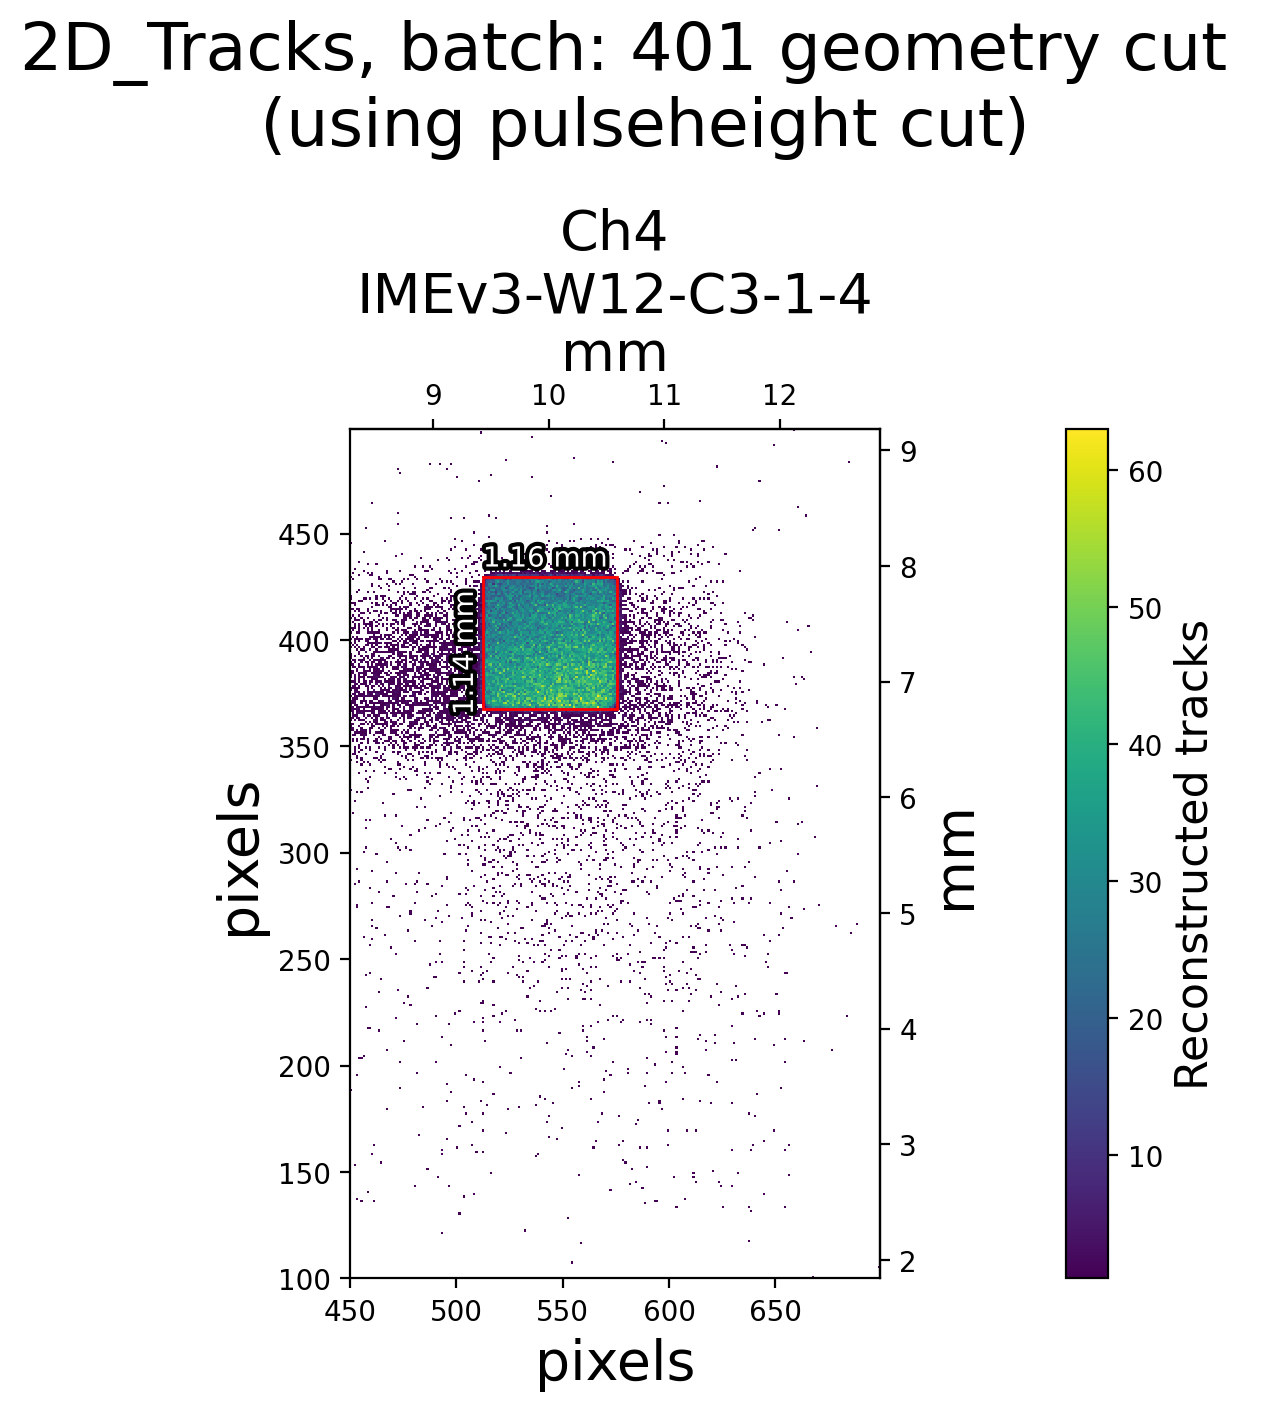
\includegraphics[width=.48\textwidth]{Images/appendix/2D_Tracks_401_S1 highlight geometry cut (using pulseHeight).png}
        \label{fig:geometry_cut_using_pulseHeight}}
    \hfill
    \centering
    \subfloat[Using time cut]{
        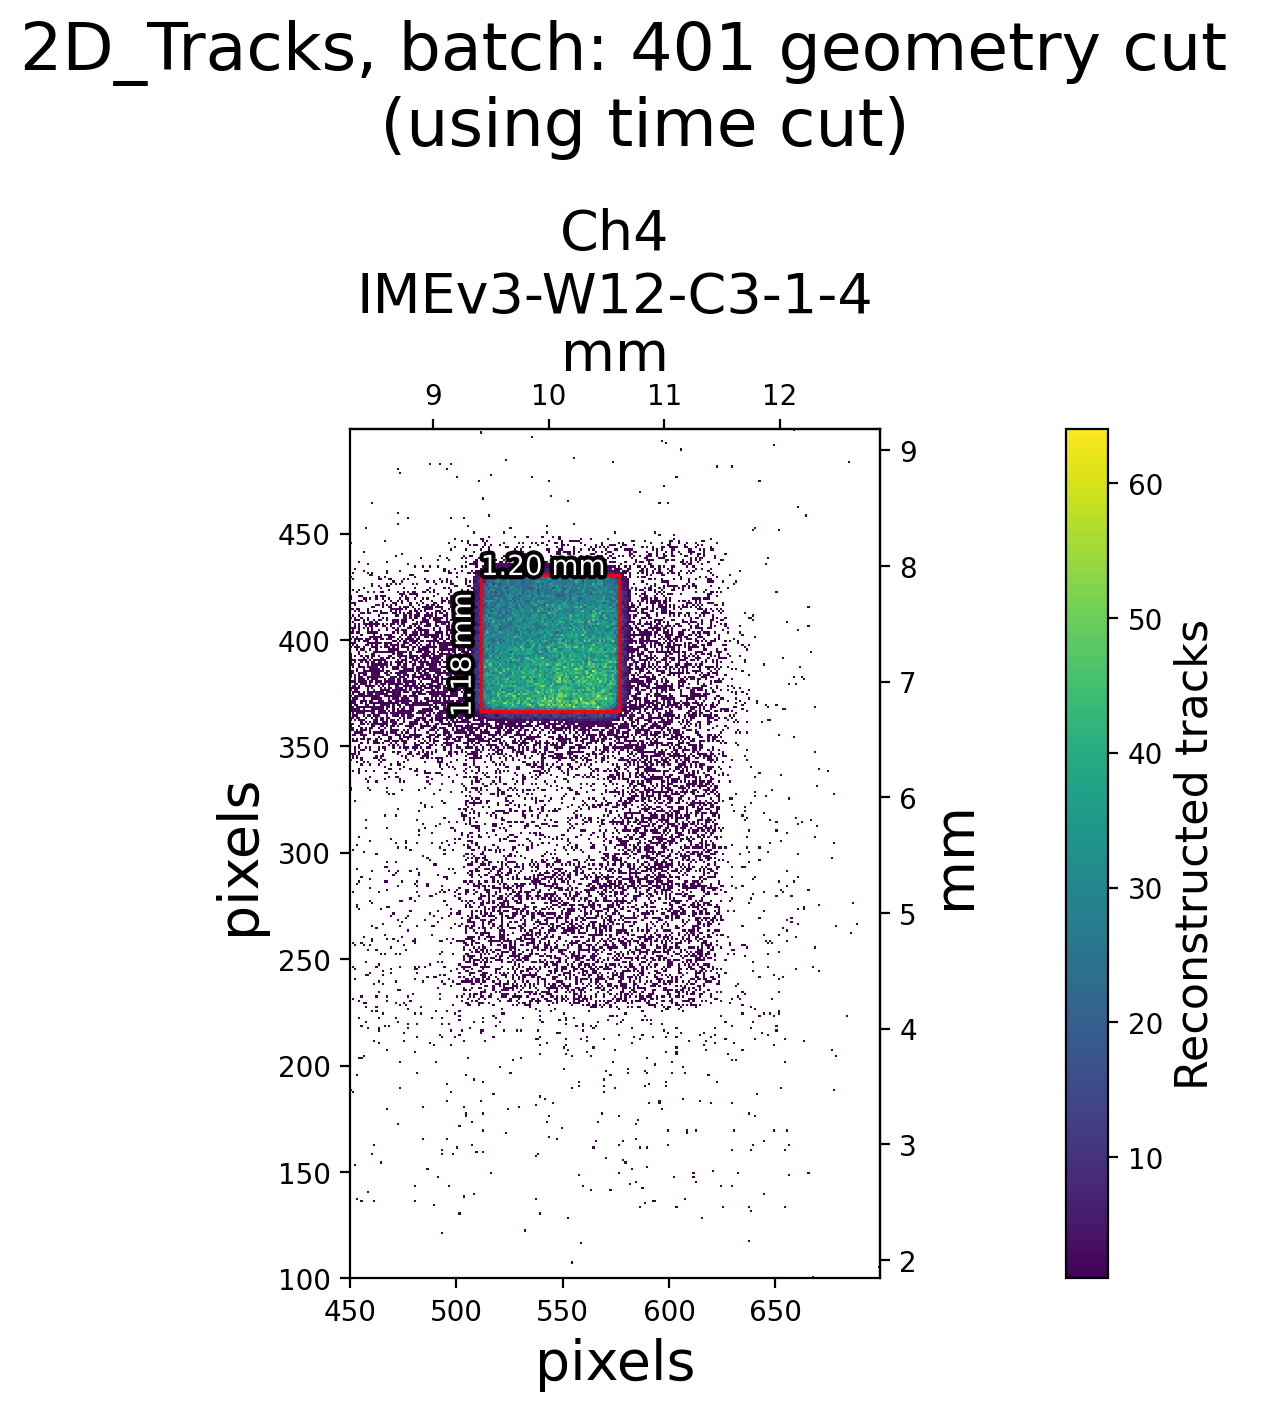
\includegraphics[width=.48\textwidth]{Images/appendix/2D_Tracks_401_S1 highlight geometry cut (using time).png}
        \label{fig:geometry_cut_using_time}}
    \caption{Example of the two \textit{geometry cuts} (red rectangles) obtained by applying two different cuts}
    \label{fig:geometry_cut_comparison}
\end{figure}

\begin{figure}[!ht]
    \centering
    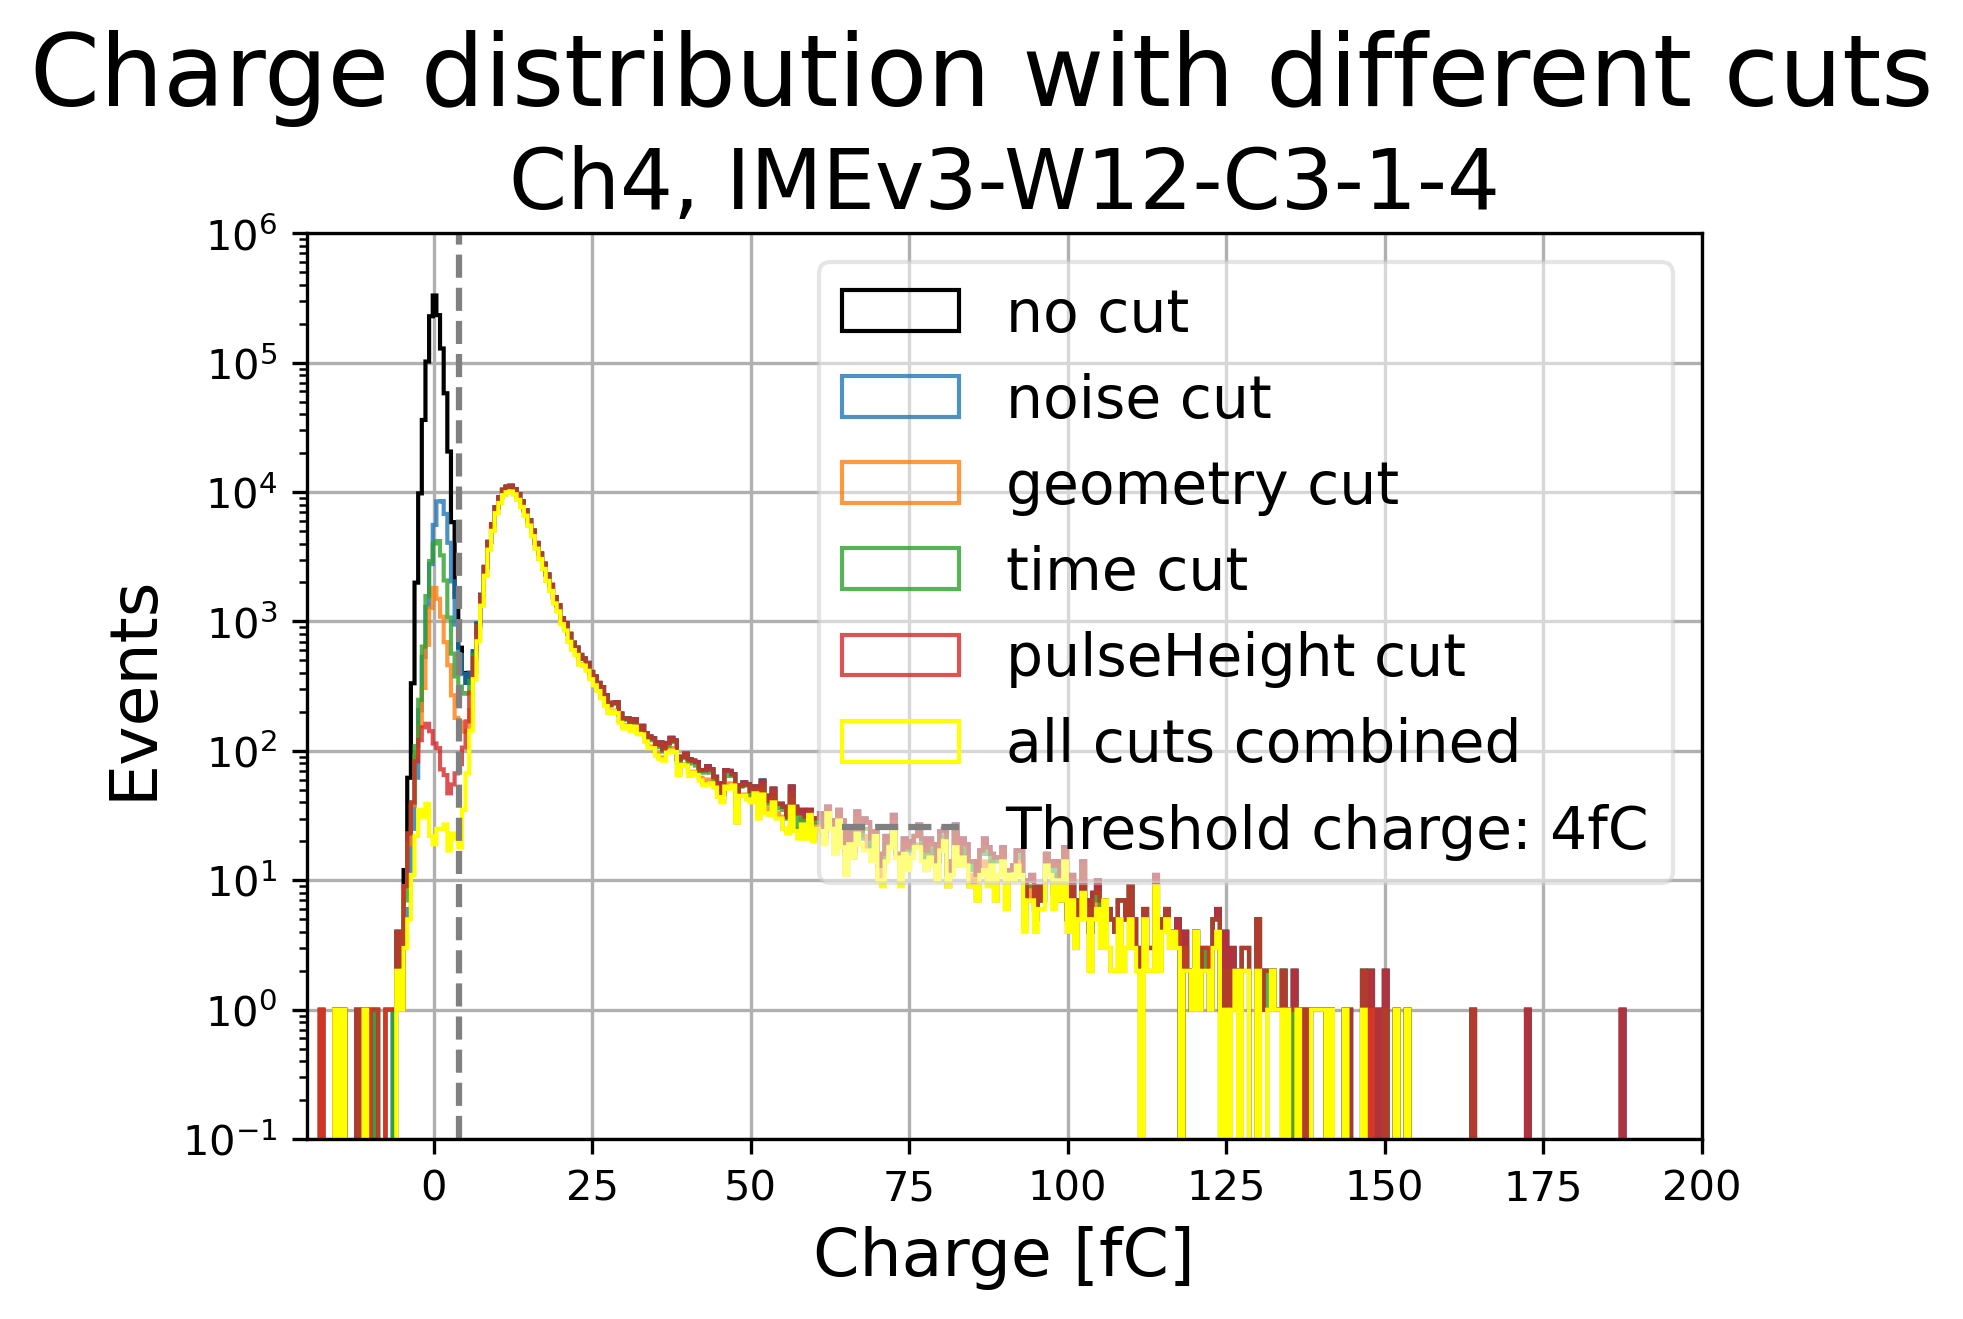
\includegraphics[width=0.7\linewidth]{Images/appendix/Charge_distribution_different_cuts_batch_401_S1_DUTs_3.png}
    \caption{The different quality cuts applied and their individual effect on the charge distribution}
    \label{fig:charge_plot_all_cuts}
\end{figure}

\printbibliography

\end{document}